\documentclass[12pt, twoside]{report}
\usepackage[T1]{fontenc}
\usepackage[linedheaders,parts,pdfspacing]{classicthesis}
\usepackage[utf8]{inputenc}
\usepackage[inner=3cm,outer=2cm,top=2cm,bottom=2cm,includehead,includefoot]{geometry}
\usepackage{graphicx}
\usepackage{xcolor}
\usepackage[numbers]{natbib}
\usepackage{setspace}
\usepackage{amsmath}
\usepackage{algorithm}
\usepackage{algpseudocode}
\usepackage{mathtools}
\usepackage{lscape}
\usepackage[toc,page]{appendix}
%\usepackage[ocgcolorlinks]{hyperref}
%\hypersetup{
%    colorlinks=true,
%    linkcolor=black, 
%    filecolor=magenta,      
%    urlcolor=cyan,
%}

%Tikz packages.
\usepackage{tikz}
\usepackage{tikz-3dplot}
\usetikzlibrary{positioning}
\usetikzlibrary{bayesnet}

%Set double spacing.
\doublespacing

% Declare some math operators.
\DeclareMathOperator*{\argmin}{arg\,min}
\newcommand{\norm}[1]{\left\lVert#1\right\rVert_{2}}
\newcommand\given[1][]{\:#1\vert\:}
\newcommand{\std}[1]{{\footnotesize $\pm${#1}}}
\newcommand{\intd}[1]{{\mathrm d{#1}}}

\title{
    {Thesis Title}\\
    \vspace{10 mm}
    {
\includegraphics[scale=1]{pre_chapters/figures/oxford_logo.png}\\
    {\large Department of Engineering Science\\ University of Oxford}\\}
}
\author{Mr Jack Miles Hunt}
\date{}

\bibliographystyle{ieeetr}
\begin{document}
\maketitle
\chapter*{Declaration}
I declare that the work contained in this Thesis is entirely my own, and except where otherwise indicated, 
describes my own research.

\chapter*{Acknowledgements}
% EPSRC, AIMS
% Phil & Victor
% Stuart & Mike
% Wendy, Niki and Steve
% Zoe
% Family
% Early education; CSS & Goldsmiths

\chapter*{Abstract}
Advances in 3D computer vision have tremendously impacted the way that humans and computers interact,
ranging from immersive, Virtual Reality video games, to industrial robotics. Such applications of 3D 
vision are underpinned by a range of computer vision competencies, including pose estimation, mapping 
and semantic understanding. However, there remain many difficult, open research problems within the field, 
such as many common mapping approaches being restricted to static environments, the difficulty in obtaining 
high quality 3D models of objects, and scene understanding and modelling in large scale environments, such as 
towns or cities.

In this Thesis, there are three central subject matters that are approached. Firstly, an approach to the 
difficult task of dense mapping in dynamic environments is proposed. Central to the approach is a novel 
representation of the observed scene that allows for dynamic components, such as walking people to be 
separately handled from their static counterparts, such as furniture. It is demonstrated in this work that 
the proposed approach yields an improvement in pose estimation accuracy in dynamic scenes, versus it's 
common, static counterpart. Additionally, the proposed approach is capable of exceeding real-time performance, 
and may be leveraged for simple geometric feature extraction for semantics due to it's motion segmentation
capability.

The second central research topic of this Thesis is the high quality reconstruction of 3D objects. 
The approach to which comprises a novel representation and formulation of the problem, such that errors are 
corrected online. The proposed approach is evaluated against a state of the art method, over which an 
improvement in reconstruction is demonstrated. Additionally, the efficacy of the online correction procedure 
is demonstrated versus a vanilla approach. Finally, high levels of geometric accuracy are seen versus an appropriate 
benchmark.

%%% SPP
%%%%%% Preliminary results indicate ambitous task may be tractable
%%%%%% Promising avenue of research yada yada
The third major focus of this work is the simultaneous inference of object shape and pose in large scale, outdoor environments. 
An ambitous approach to regressing shape and pose in a weakly-supervised manner is presented, utilising a combination 
of Convolutional Neural Networks and Gaussian Processes. Early results indicate\dots

The work that is outlined in this Thesis is intended to provide a strong foundation for further research in the area of 
geometrically driven 3D scene understanding. However, immediate applications are evident. The motion segmentation and 
dense mapping approach for dynamic environments allows for larger scale dense mapping in previously prohibitive scenarios, 
and as such has applications in robotics. The object reconstruction work that constitutes the second major focus of the Thesis 
is applicable to the problem of collecting geometrically consistent 3D object data. Finally, the simultaneous inference of 
shape and pose is applicable to modelling scenarios of specific semantic interest, where an entire scene need not be reconstructed. 
The approach preliminarily demonstrates potential for large scale, semi-dense, geometric and semantic mapping.

\chapter*{Notation and Abbreviations Used}
\section*{Mathematical Notation}
This preliminary section introduces the mathematical notation used in this work. The following 
table outlines essential notational details, separated into sections on Sets, Fields and Groups, 
Linear Algebra, Sums and Products, Calculus and Probability Theory.
\begin{longtable}{p{.20\textwidth} | p{.8\textwidth}}
  \hline
  Symbolic Form & Meaning \\
  \hline
  \( \mathcal{A} \) & Calligraphic variables indicate mathematical sets (unless otherwise indicated).\\
  \( \{ a, b, c \} \) & A mathematical set consisting of the elements \( a \), \( b \) and \( c \).\\
  \( \{ a | \rho(a) \} \) & A mathematical set whose elements are defined by predicate \( \rho(a) \).\\
  \( a \in \mathcal{A} \) & The element \( a \), in the set \( \mathcal{A} \).\\
  \( f(a) \forall a \in \mathcal{A} \) & \( f(a) \) for all \( a \) in \( \mathcal{A} \).\\
  \( | \mathcal{S} | \) & Cardinality of \( \mathcal{S} \); the number of elements in \( \mathcal{S} \).\\
  \( \inf \mathcal{S} \) & Infimum of \( \mathcal{S} \).\\
  \( \sup \mathcal{S} \) & Supremum of \( \mathcal{S} \).\\
  \hline
  \( \mathbb{R}^{N} \) & The field of real numbers, of dimension \( N \).\\
  \( \mathbb{SE}(3) \) & The Special Eucledian Group of \( 4 \times 4 \) transform matrices.\\
  \( \mathbb{SO}(3) \) & The Special Orthogonal Group of \( 3 \times 3 \) rotation matrices.\\
  \hline
  \( \bm{A}\), \( \bm{\Theta} \) & Bold, uppercase symbols indicate matrix or tensor quantities.\\
  \( \bm{a}\), \( \bm{\theta} \) & Bold, lowercase symbols indicate vector quantities.\\
  \( \lVert \bm{a} \rVert_{n} \) & \( n \)-norm of a vector.\\
  \( \bm{a}^{T} \), \( \bm{A}^{T} \) & Transpose of a vector or matrix.\\
  \( \bm{A}^{-1} \) & The matrix inverse of \( \bm{A} \).\\
  \( \text{tr}(\bm{A}) \) & Trace of the matrix \( A \).\\
  \hline
  \(\sum_{a = 0}^{N} a\) & The sum from \( 0 \) to \( N \) of \( a \).\\
  \(\sum_{a \in \mathcal{A}}\) & The sum of the elements in \( \mathcal{A} \).\\
  \(\prod_{a = 0}^{N} a\) & The product from \( 0 \) to \( N \) of \( a \).\\
  \hline
  \( \frac{\partial f(\bm{a})}{\partial \bm{a}_{i}} \) & Partial derivative of \( f \) with respect to the \( i^{th} \) element of \( \bm{a} \).\\
  \( \nabla f(\bm{a}) \) & Gradient vector of \( f(\bm{a}) \). The vector of partial derivatives.\\
  \( \int f(a) \intd a \) & Infedinite integral over \( f(a) \) with respect to \( a \).\\
  \( \int_{m}^{n} f(a) \intd a \) & Definite integral over \( f(a) \) with respect to \( a \), between \( m \) and \( n \).\\
  \hline
  \( P(a, b, c) \) & Joint distribution over the random variables \( a \), \( b \) and \( c \).\\
  \( P(a \given b, c) \) & Distribution over the random variable \( a \), conditioned on \( b \) and \( c \).\\
  \( P(a) \) & Marginal distribution over the random variable \( a \).\\
  \( \mathcal{N}(a \given \mu, \sigma) \) & Gaussian distribution parameterised by mean \( \mu \) and standard deviation \( \sigma \).\\
  \( \mathcal{N}(\bm{a} \given \bm{\mu}, \bm{\Sigma}) \) & Multivariate Gaussian distribution parameterised by mean \( \bm{\mu} \) and covariance \( \bm{\sigma} \).\\
  \( \mathbb{E}(a) \) & Expectation over the random variable \( a \).\\
  \( b \sim P(a) \) & A sample \( b \), drawn from the distribution \( P(a) \).\\
  \( f(a) \sim \mathcal{GP}(a) \) & A function \( f(a) \), drawn from the Gaussian Process \( \mathcal{GP}(\bm{\mu}), \bm{\Sigma} \).\\
  \( \mathbb{KL}(P(a) \given P(b)) \) & KL Divergence from the distribution \( P(a) \) to the distribution \( P(b) \).\\
  \( \mathbb{JSD}(P(a) \given P(b)) \) & Jensen-Shannon Divergence between the distributions \( P(a) \) and \( P(b) \).
~\label{table:mathematical_notation}
\end{longtable}

\section*{Abbreviations}
In this preliminary section, a reference of abbreviations used in this work is given. The 
abbreviations and their associated meanings are given in the following table. Note that 
abbreviations that are used only in the literature review of Chapter~\ref{chap:lit_review} 
are excluded. Abbreviations are listed in order of first appearance in the text.
\begin{longtable}{p{.20\textwidth} | p{.8\textwidth}}
  \hline
  Abbreviation & Meaning \\
  \hline
  3D & Three Dimensional.\\
  VR & Virtual Reality.\\
  AR & Augmented Reality.\\
  RGB & Red-Green-Blue.\\
  RGBD & Red-Green-Blue-Depth.\\
  SLAM & Simultaneous Localisation and Mapping.\\
  AI & Artificial Intelligence.\\
  ML & Machine Learning.\\
  GPU & Graphical Processing Unit.\\
  SDF & Signed Distance Function.\\
  \hline
  TSDF & Truncated Signed Distance Function.\\
  ICP & Iterative Closest Points.\\
  ATE & Absolute Trajectory Error.\\
  RTE & Relative Trajectory Error.\\
  RMSE & Root Mean Squared Error.\\
  SVM & Suport Vector Machine.\\
  FPFH & Fast Point Feature Histogram.\\
  \hline
  CRF & Conditional Random Field.\\
  MLE & Maximum Likelihood Estimate.\\
  PDF & Probability Density Function.\\
  PMF & Probability Mass Function.\\
  CDF & Cumulative Density Function.\\
  PwP & Pixel-wise-Posteriors.\\
  PGM & Probabilistic Graphical Model.\\
  MAP & Maximum a Posteriori.\\
  CNN & Convolutional Neural Network.\\
  GP & Gaussian Process.\\
  GPLVM & Gaussian Process Latent Variable Model.\\
  DCT & Discrete Cosine Transform.\\
  IDCT & Inverse Discrete Cosine Transform.\\
  PCA & Principal Component Analysis.\\
  KL & Kullback-Leibler (Divergence).\\
  JSD & Jensen-Shannon Divergence.
~\label{table:abbreviations}
\end{longtable}

\tableofcontents
\listoffigures
\listoftables

\chapter{Introduction}
% Introduction of Introduction
% -- Increased compute changed how people interact with computers
% ---- Games to social media, medical imaging to service robotics
% ---- Immersive virtual worlds - VR
% ---- Virtual to real world - AR
% -- The above is enriched by vast amounts of data and modern ML
% ---- Semantics, detections etc
% -- 3D sensing equipment allows for geometric modelling of real world
% ---- Reconstructions, 3D motion estimation, pose tracking
% ---- 3D sensing combined with ML allows for rich scene understanding; link back to VR/AR
% ---- 3D data not in abundance, unlike 2D images; harder to train task specific systems
Much has changed since the introduction of the IBM PC platform in 1981, with regards to the 
uses of the Personal Computer and the way in which humans interact with them. Vast increases 
in computational power have seen the microcomputer evolve beyond a tool with which one predominantly 
collated data with spreadsheets (``VisiCalc'' is widely accepted to be the first \textit{killer app}
for the PC). At present, personal computing is ubiquitous, providing the means for activities ranging 
from playing visually realistic 3D games, to sharing life events online with friends and family via 
so called ``Social Media'' platforms. Advances in graphics processing power have lead to the introduction 
of many technologies that both the public sector and private enterprises have come to depend on, from 
sophisticated medical image analysis, to robotic production lines.

The aforementioned vast power of the modern GPU (Graphical Processing Unit) has lead to the development 
of new ways for humans to interact with computers, and for computers to interact with the world. Advances 
in VR (Virtual Reality) allow humans to experience digital worlds in a fully immersive manner, with 
applications ranging from gaming, to experimental therapeutic treatment of Paranoid Schizophrenia. 
Whereas AR (Augmented Reality) allows a person to supplement their perception of the tangible world with 
elements of the digital, by viewing the world through a computer system that percieves and adds synthetic 
components. Common applications of AR include digital interior design and smartphone games.

Many of the aforementioned advancements in the applications of and interactions with modern computer 
systems are driven by Artificial Intelligence (AI). Modern AI provides much of the semantic and contextual 
information required to make meaningful inferences over the state of the world, as observed by a sensor 
(such as a camera) attached to such a computer system. Much advancement has been made in recent years on 
the tasks of object detection and semantic understanding in standard, 2D images. However, there are many 
technical challenges that must be overcome before such efficacy on these tasks is reached for the 3D 
case.



% Topic overview.
% -- 3D machine perception
% ---- optical flow
% ---- laser range sensing
% ---- navigation and mapping with sparse point clouds
% ---- stereo and rgbd
% ---- multiple view geometry
% ---- SfM, SLAM, scene flow
% -- Semantics
% ---- object recognition and segmentation
% ---- user interaction
% -- Amalgamation
% ---- applications in VR/AR
% ---- ad-hoc ML (3d data procurement etc)
% -- Current challenges
% ---- fragility in complex, real environments (dynamics etc)
% ---- lack of real world data for learning of 3d
% ---- SLAM limited to observations only; may not see whole thing; may not be practical etc

% Elaborate on current challenges.
% -- Dynamics in SLAM
% ---- for SLAM in real environments (working environments such as warehouses), no consistent model
% ---- fragility leads to problems; complete failure to inaccuracies
% ---- reliance on point correspondences; efficacious for static, fails for dynamic
% ---- no dynamics = limited perception capability; needed for "real" environments
% ---- dynamics provide semantic information
% -- Object centric SLAM/SfM
% ---- preliminary work limited on simultaneous TaM; offline or known pose
% ---- fundamentally a difficult problem; less to work with
% ---- geometric inconsistencies more pronounced effect; bad training data etc
% -- Data driven pose/shape regression
% ---- complex environments may not allow long enough to fuse model
% ---- larger scale makes dense reconstruction infeasable
% ---- limited observability; not able to fully cover object
% ---- eliminate many lower level "tricks" to make reconstruction work

% Research questions.
% -- Can we reconstruct densely in dynamic scenes?
% ---- real time?
% ---- comparable reconstruction quality to state of art?
% ---- can we improve tracking in these scenarios?
% -- Can we determine what is dynamic in a scene?
% ---- Can we leverage this information in some semantic way (link back to AR applications/data collection)?
% -- Can we obtain consistent reconstructions of arbitrary objects?
% ---- comparable reconstruction quality to state of the art scene based?
% ---- with commodity hardware?; wider applicability
% ---- without known pose?
% ---- 
% -- Can we infer scene properties where traditional reconstruction not possible?
% ---- shape and pose?
% ---- without requiring temporal consistency?; avert tracking errors
% ---- 

% Thesis roadmap.
% -- Literature review.
% ---- TaM/SLAM
% ---- Semantics/Semantic SLAM
% ---- Dynamics, moseg and optical flow
% ---- Object reconstruction
% ---- Shape and pose regression
% -- "Real Time Motion Segmentation for Dense Volumetric Fusion"
% ---- Outline preliminaries; standard dense SLAM etc
% ---- Approach to dynamic dense SLAM
% ---- Segmentation of dynamics; which questions adressed?
% ---- Rudimentary example of semantics; which questions adressed?
% ---- Outline experiments
% ---- Results showing...
% -- "Probabilistic Object Reconstruction with Online Drift Correction"
% ---- Outline approach; which questions adressed?
% ---- Outline experiments
% ---- Outline results
% -- "Stereo Shape and Pose Regression"
% ---- Outline approach; which questions adressed?
% ---- Outline experiments
% ---- Outline results

\chapter{Literature Review}
%%% Local Variables: 
%%% mode: latex
%%% TeX-master: "../thesis"
%%% End: 

%% Tracking and Mapping.
\section{Tracking and Mapping}
\label{sec:lit_review_tam}
There has been much research in the field of Tracking and Mapping in recent 
years, with many large scale works being driven by the availibility of once 
costly depth sensing equipment. The availability of such equipment combined 
with the ever increasingly parallel nature of modern GPU's has seen the 
field advance greatly beyond the seminal but resource limited works of it's 
infancy. This advancement is most predominant within the Dense SLAM(Simultaneous 
Localisation and Mapping) literature. This section shall first explore the 
earlier, fundamental works of this area of research, followed by a treatment 
of the current state of the art.

\textit{Besl \& McKay} \cite{Besl1992} introduced their seminal work on 3D shape 
registration in 1992, providing a method to estimate full 6DoF(Six Degrees of 
Freedom) pose between 3D point sets. The authors present an Iterative Closest 
Point Algorithm that consists of three operations per iteration; computation 
of closest point, computation of a 6DoF Transformation and application of 
the Transformation. The authors present a proof of convergence based on that 
of Least Squares minimisation, however there must be sufficiently complex 
geometry present in the structure of the data to optimise to a meaningful 
Transformation.

Complementary to the aforementioned works of \textit{Besl \& McKay} \cite{Besl1992} 
in the foundational aspects of Dense SLAM is that of \textit{Curless \& Levoy} 
\cite{Curless1996}, 1996. The authors present an early volumetric integration 
framework for the reconstruction of shapes from range data obtained from a 
sensor such as a laser scanner. The authors introduce the SDF(Signed Distance Function), 
a volumetric, implicit shape representation in which entries are cumulatively updated 
in a weighted manner. Once observations have been integrated in to the SDF volume, an 
Isosurface representation of the shape is extracted by a Marching Cubes \cite{MC} 
procedure. Though the approach may lead to gaps in the resultant model, the authors 
mitigate this by introducing a Surface Tesselation step.

Later work by \textit{Zhou et al} \cite{Zhou2008} in 2008 introduces an alternative 
shape representation to that of \textit{Curless \& Levoy} \cite{Curless1996}, based 
on the spatial KD-Tree data structure and a highly data parallel BFS(Breadth First 
Search) construction algorithm. The level of parallelism introduced allows for 
application to problems that require real time performance. The authors provide 
examples of use in Ray Tracing \cite{RT} and Photon Mapping \cite{PM}.

In the same year, \textit{Censi} \cite{Censi2008} introduced \textit{PL-ICP}, a 
variant of the ICP algorithm introduced by \textit{Besl \& McKay} \cite{Besl1992}. 
The presented approach utilises a Point-to-Line metric rather than a Point-to-Point 
metric and has a closed form solution in the planar case. For the non planar case 
the presented approach acheives quadratic convergence in a finite number of steps, 
utilising a Normal weighting and a Lagrangian optimisation scheme. However, it is 
highlighted that prior to the optimisation procedure it is necessary to trim outliers 
from the point data sets.

Culminating much of the aforementioned work, in 2011 \textit{Newcombe et al} introduced 
the seminal \textit{KinectFusion} pipeline, allowing for real time mapping of indoor 
scenes with the Kinect RGBD sensor from Microsoft. The authors utilise a sparser form 
of the SDF structure introduced by \textit{Curless \& Levoy} \cite{Curless1996}, the 
TSDF(Truncated Signed Distance Function), allowing for reconstruction at scene scale. 
For pose estimation, a multi-level variant of the ICP algorithm utilising a Point-to-Plane 
metric similar to that of \textit{PL-ICP} \cite{Censi2008} is used. The pipeline consists 
of four phases; \textit{Measurement}, \textit{Integration}, \textit{Isosurface Extraction} 
and \textit{Pose Update}. Applications of the presented system however are limited only to 
those that require the reconstruction of static scenes; dynamic scenes are not supported 
by \textit{KinectFusion}.

Further optimisations were made in 2013 by \textit{Nei{\ss}ner at al} to the \textit{KinectFusion} 
pipeline proposed by \textit{Newcombe et al}. The authors introduce a spatially hashed TSDF data 
structure, in which the TSDF is split in to hashed Voxel Blocks allowing for very fast Voxel 
lookups. The presented approach yields low space and time complexity for such operations, vastly 
increasing the potential for real time, large scale use. Additionally, a streaming system is 
introduced to dynamically handle data transmission between the CPU and GPU, allowing for the 
reconstruction of scenes that may exceed the GRAM bounds of commodity GPU's. The proposed 
system is capable of running at $\approx46Hz$ on an NVIDIA Titan GPU.

In the same year, \textit{Thomas et al} \cite{Thomas2013} introduced an alternative scene 
representation, based on the notion that a scene may be represented as a set of Planar 
components with attributes such as Surface Normals, confidences and RGB colour. The motivation 
of the author's approach is that many common scenes that one might reconstruct are indoors and 
consist of components that are planar in nature, such as walls, floors and ceilings. Additionally, 
many planar objects are common, such as tables and cabinets. The author presents an alternative 
rendering approach based on Quadrangulation \cite{QUAD} and utilise a \textit{KinectFusion} 
\cite{Newcombe2011} like ICP based algorithm for pose estimation.

\textit{Salas-Moreno et al} \cite{Salas-Moreno2013} in 2013 also, introduced another alternative 
approach to that of the \textit{KinectFusion} \cite{Newcombe2011} like pipelines that similarly to 
\textit{Thomas et al} \cite{Thomas2013}, utilises the prior information that many scenes consist 
of predictable, repeated structures. As such, the authors introduce a so called ``Object Oriented'' 
Dense SLAM paradigm, in which the reconstruction of the scene is split in to a graph of observed 
objects. Pose estimation is achieved by running an ICP based algorithm against renderings of the 
individual objects in the reconstructed scene model. Following pose estimation, the proposed 
system detects newly observed objects and inserts the appropriate object model in to the scene 
model. Consistency between scene components is enforced with Pose Graph Optimisation, with 
relocalisation achieved in a similar manner. The proposed approach does however require a 
database of known objects a-priori.

\textit{St{\"u}ckler et al} \cite{Stuckler2014} in 2014 introduced a non implicit, non volumetric 
representation based on multiple resolution Surfel \cite{Pfister2000} Maps. The core data structure 
used for scene representation is a Voxel Octree \cite{OCTREE} containing both Surfels and 
Probability Distributions over appearance and shape. Pose estimation is achieved by optimising for 
a Unit Quaternion \cite{QUAT} and Translation Vector within a Maximum Likelihood framework, in which 
the Energy Function to be maximised is the Likelihood of the RGBD observations given the accumulated 
Probability Distributions stored in the Octree. The presented pipeline also incorporates a randomised, 
graph and keyframe based loop closure component.

Salas-Moreno et.al. \cite{Salas-Moreno2014}
\begin{itemize}
	\item Exploits planar structure in the scene, like Thomas.
	\item Focus on detection and modelling of planes, refined over time.
	\item From generated Surfel maps, planes are segmented and holes filled over time. \cite{Pfister2000}
	\item Fern encoding used for relocalisation. %Reference Fern Encoding - Glocker et al
	\item ICP between measured vertex map and predicted vertex map.
\end{itemize}

Prisacariu et.al \cite{Prisacariu2014} Followed up by tech report \cite{Kahler2015}
\begin{itemize}
	\item Open source implementation of Voxel Hashing.
	\item A number of optimisations to the data structure(allocation \& integration) and raycaster.
	\item IMU data to supplement camera observations for tracking.
	\item 47Hz NVIDIA Shield tablet, 910Hz Titan X.
\end{itemize}

Whelan et.al \cite{Whelan2015}
\begin{itemize}
	\item Like KF but large scale(hundreds of meters), achieved using GPU cyclic buffers.
	\item Geometric and photometric camera pose constraints.
	\item Map updated by frame recognition, as-rigid-as-possible. %Reference as-rigid-as-possible
	\item Pose graph based loop closure.
\end{itemize}

Zhou et.al. \cite{Zhou2015}
\begin{itemize}
	\item Uses contour cues to improve camera tracking.
	\item Contour cues extracted from noisy and incomplete depth images.
	\item Correspondence constraints using scene geometry enforced on pose estimation.
	\item Based on KF pipeline.
	\item Depth image inpainting used before contour extraction.
\end{itemize}

%TO-DO: fix name.
Kahler et.al \cite{Kahler2016} 
\begin{itemize}
	\item Based on KF pipeline and InfiniTAM.
	\item Online submap alignment algorithm for drift correction.
	\item Inter-submap corrections based on graph optimisation.
	\item Loop closure detected using fern conservatories. %cite glocker
\end{itemize}

%% Semantic SLAM.
\section{Semantic SLAM}
\label{sec:lit_review_semantic}
Civera et.al. \cite{Civera2011}
\begin{itemize}
	\item Monocular EKF based SLAM.
	\item Semantics added to points via SURF correspondences with precomputed object descriptors.
	\item Geometric compatibility is then tested.
\end{itemize}

%TO-DO: fix name,
Stuckler et.al \cite{Stuckler2012} 
\begin{itemize}
	\item Uses RGB-D, not monocular.
	\item Fuses only detected objects.
	\item Object detection via random forests.
	\item Hand crafted features over object regions.
\end{itemize}

Valentin et.al. \cite{Valentin2015} Golodetz et.al. \cite{Golodetz2015}.
\begin{itemize}
	\item Online, real time semantic segmentation using user input.
	\item Dense reconstruction like KF.
	\item User physically interacts.
	\item Voxel Oriented Patch features using normals and appearance in CIELab.
	\item Streaming Random Forests\cite{Abdulsalam2007}  and Valentin version uses Mean Field \cite{Xing2002} optimised by \cite{Krahenbuhl2011}.
\end{itemize}

Bengio et.al. \cite{Bengio2013} - representation learning.
Girshick et.al \cite{Girshick2014} - feature hierarchies.
Handa et.al. \cite{Handa2015}
\begin{itemize}
	\item Real time reconstruction with semantic segmentation.
	\item Deep autoencoders stacked and trained on synthetic depth data.
	\item Uses depth only cues.
	\item KF style reconstruction.
\end{itemize}

Cavallari et.al. \cite{Cavallari2016}
\begin{itemize}
	\item Built on top of Voxel Hashing
	\item RGB frames passed to FCN\cite{Shelhamer2017}, PMF's out.
	\item Post rendering, colours determined by argmax over PMF bins.
	\item Texture(non label colours) trilinearly interpolated.
\end{itemize}

%% Dynamic SLAM.
\section{Dynamic SLAM, Motion Segmentation and Optical Flow}
\label{sec:lit_review_dynamic}
Tsap et.al. \cite{Tsap2000}
\begin{itemize}
	\item Algorithm for nonrigid motion tracking.
	\item Solve for dense motion vector fields between 3D objects via Finite Element Methods. %Cite FEM
	\item Iteratively analyses difference between actual and predicted behaviour.
	\item Iterative descent to find optimal parameters of nonlinear FEM.
	\item Tracking improved by using point correspondences.
	\item Not scene based.
\end{itemize}

Chen et.al \cite{Chen2011}
\begin{itemize}
	\item Nonrigid motion tracking applied to human body.
	\item Surface mesh extracted from multi view video and skinned.
	\item Hierarchical(w.r.t articulation) Weighted ICP is then applied.
	\item ICP points weighted by Approximate Nearest Neighbour %cite
	\item Prior human skeleton fitted.
	\item Not scene based.
\end{itemize}

Sun et.al. \cite{Sun2012}
\begin{itemize}
	\item Layered optical flow. Layered over detected moving objects.
	\item Depth ordered MRF's and Max Flow used for layering.%cite MF
	\item Number of layers automatically determined.
	\item Max Flow used to solve for discretised flow field cost function.
	\item Motion tracking only, no reconstruction.
\end{itemize}

Unger et.al. \cite{Unger2012}
\begin{itemize}
	\item Variational formulation for motion estimation and segmentation with occlusion handling.
	\item Parametric labelling of flow field for each object undergoing motion.
	\item Labels encoded with an MRF Potts model as with Sun. %cite potts model.
	\item Flow and labels solved for via Primal-Dual optimisation framework. %cite primal dual
	\item Again, motion only. No reconstruction.
\end{itemize}

Herbst et.al. \cite{Herbst2013}
\begin{itemize}
	\item Extension of Optical Flow to 3D scenes.
	\item Scene flow computed from RGB-D data, i.e. Kinect.
	\item Approach based on Brox et.al. \cite{Brox2004}
	\item Variational formulation and optimisation framework.
\end{itemize}

Stuckler et.al. \cite{Stueckler2013}
\begin{itemize}
	\item EM framework to segment rigid body motion from RGBD data.
	\item Robust to simultaneous fg and bg motion by treating both with parity.
	\item Sites of motion as well as motion params are posed as latent variables.
	\item No reconstruction, but feasibly could be extended.
\end{itemize}

Keller et.al. \cite{Keller2013}
\begin{itemize}
	\item Dense SLAM system capable of handling scene dynamics.
	\item Works with RGB-D data.
	\item Uses ICP outliers to determine dynamic scene components followed by flood fill.
	\item Surfel representation \cite{Pfister2000}
	\item Flat data structure. Does not have advantages of Voxel Hashing.
\end{itemize}

Perera et.al. \cite{Perera2015}
\begin{itemize}
	\item Motion segmentation in TSDF volumes,
	\item Based on MAP inference over a CRF on the TSDF.
	\item Can handle minor and major displacements.
	\item Motion labels and parameters found w.r.t. live frame and TSDF.
	\item $256^{3}$ voxel grid does not run real time. Scalability issues.
\end{itemize}

Newcombe et.al. \cite{Newcombe2015}
\begin{itemize}
	\item Handles non-rigidly deforming scenes.
	\item Built on KinectFusion pipeline.
	\item 6DoF motion field estimated that warps model to live frame.
	\item Warp field used to fuse new measurements in to canonical model.
	\item Warp field solved for by Dual Quaternion Blending. \cite{Kavan2006}
	\item Limitations, such as lack of robustness to open/closed topology changes(hands). Authors highlight scalability issues.
\end{itemize}

%% Object Reconstruction.
\section{Object Reconstruction}
\label{sec:lit_review_obj_recon}
Curless and Levoy \cite{Curless1996}
\begin{itemize}
	\item Object reconstruction from different viewpoints but statically.
	\item No pose tracking in the TAM sense.
\end{itemize}

Kolev et.al. \cite{Kolev2006}
\begin{itemize}
	\item Probabilistic 3D segmentation.
	\item Rather than direct reconstruction like Curless, the most probable image w.r.t. images is inferred.
	\item Level set representation used.
	\item Level set has analogous probability volume(pF,pB)
	\item Level set is evolved via a variational framework over probability volume.
	\item Only evaluated on synthetic data.
	\item Designed for objects with distinct appearance and homogeneous background, though some tolerance to noise is claimed.
\end{itemize}

Weise et.al. \cite{Weise2009}
\begin{itemize}
	\item 3D in hand scanning system.
	\item Point cloud representation, Surfel rendering. \cite{Pfister2000}
	\item Objects rotated in front of a sensor, suggests limited tracking ability.
	\item Drift offset in as-rigid-as-possible manner. %cite as-rigid-as-possible
	\item ICP registration. Topology graph used for deformation.
	\item Uses range scanner. No indication of RGBD capability. May need high quality equipment.
\end{itemize}

Ren et.al. \cite{Ren2013}
\begin{itemize}
	\item Probabilistic framework for tracking and reconstruction of objects.
	\item Initialised with a shape prior level set, which is then evolved as per observations.
	\item Works with RGBD data.
	\item Pixel-Wise-Posteriors used for segmentation. Prob volume like Kolev. \cite{Bibby2008}
	\item Experiments show limitations.
\end{itemize}

Dou et.al. \cite{Dou2015}
\begin{itemize}
	\item Reconstruction of deformable objects with a Kinect sensor.
	\item Loop closures automatically detected, distributing drift error over the loop.
	\item Latent shape and nonrigid deformation solved for with bundle adjustment.
	\item Surface represented as a triangular mesh.
	\item Experiments show high quality reconstructions, but with overnight run times.
\end{itemize}

Gupta et.al. \cite{Gupta2016}
\begin{itemize}
	\item 3D reconstruction and segmentation of objects with an RGBD sensor.
	\item Implicit representation, i.e. volumetric. Fusion with Softmax rather than weighted average like KF.
	\item Each voxel gets a label{obj, bg, empty}. Segmentation with graph cut and alpha expansion.
	\item Keyframe based loop closure.
	\item Pose estimation via photometric loss. Authors report drift to be a problem.
	\item Authors report difficulty in building a granular reconstruction.
\end{itemize}

%% Object Shape Prediction.
\section{Shape and Pose Prediction}
\label{sec:lit_review_prediction}

Prisacariu et.al. \cite{Prisacariu2011}
\begin{itemize}
	\item Shape prediction, segmentation(optimisation based) and pose optimisation.
	\item Hierarchical(early deep?) GPLVM's for Shape Latent Space Embedding. \cite{Lawrence2005}
	\item Unified energy function.
	\item Candidate shapes generated as one off regression in latent space.
\end{itemize}

Dame et.al. \cite{Dame2013}
\begin{itemize}
	\item Dense object reconstruction from monocular image source.
	\item Shape priors used to aid reconstruction and segmentation, GPLVM.
	\item Depth maps optimised for with Primal Dual with TV. Poses are known from PTAM.
\end{itemize}

Toshev et.al. \cite{Toshev2014}
\begin{itemize}
	\item Human pose estimation(articulated estimation) with Deep Neural Networks.
	\item Cascaded DNN regressors.
	\item No reconstruction, pose estimation only.
\end{itemize}

Wohlhart et.al. \cite{Wohlhart2015}
\begin{itemize}
	\item 3D object detection and pose recovery.
	\item CNN descriptors used with Nearest Neighbour Cost for detection and rough pose.
	\item Problem posed as KNN search in Descriptor Space.
	\item Object and Pose are coupled in training(i.e. two similar cars with different poses have distant descriptors)
\end{itemize}

Chang et.al. \cite{Chang2015}
\begin{itemize}
	\item Large scale dataset of 3D shapes.
	\item Synthetic data with no "source" sequence, i.e. no depth.
	\item Can be used to learn rich latent space embeddings.
\end{itemize}

Rock et.al. \cite{Rock2015}
\begin{itemize}
	\item Recovers a complete 3D model from a depth image of an object.
	\item Input depth image matched to database of objects via a Random Forest.
	\item Matched shape coarsely matched to depth map, then deformed at a higher granularity.
	\item Deformation manually optimised for.
\end{itemize}

Zhou et.al. \cite{Zhou2017_2}
\begin{itemize}
	\item Object detection from 3D Point Clouds.
	\item End-to-end trainable Convolutional, Region Proposal Network.
	\item Trained on KITTI LIDAR dataset. \cite{Geiger2013}
	\item Voxelisation of point cloud used for region detections.
\end{itemize}

Gwak et.al \cite{Gwak2017}
\begin{itemize}
	\item GAN like shape prediction with log-barrier ojective.
	\item Weakly supervised with sillhouettes and 3D shapes.
	\item May not work "in the wild"
\end{itemize}



\chapter{Real Time Motion Segmentation for Dense Volumetric Fusion}
~\label{chap:moseg}
\begin{chapterabstract}
This chapter introduces an approach to motion segmentation and dense reconstruction 
in dynamic scenes with RGBD observations.
\end{chapterabstract}

\section{Introduction}
~\label{sec:moseg_introduction}
Progress in dense volumetric fusion has been accelerated in recent years with
the availability of comsumer grade RGBD sensors such as the Microsoft Kinect and
the Asus Xtion coupled with the increasingly parallel nature of Grapical Processing 
Unit (GPU) hardware. Systems such as the seminal KinectFusion~\cite{Newcombe2011} 
allow one to build high quality, globally consistent scene models trivially, as 
outlined in Section~\ref{sec:intro_scene_recon} and Figure~\ref{figure:room_recon_example}.
Applications of such reconstruction pipelines however are limited due to the 
inability of such systems to handle scenes in which there are dynamics; such 
systems are unable to yield reliable reconstructions when there is motion in the 
sensors field of view independent of the sensors own motion. Such a scenario introduces
additional error to the pose estimation component in the pipeline and as such
causes model corruption ranging from noise in the reconstruction to spurious 
surface data due to erroneous pose estimation.

In this chapter an approach to mitigating the problems present when performing 
dense volumetric reconstruction in dynamic scenes is presented. Central to the
pipeline is the introduction of a dual scene representation based on the use
of an implicit TSDF~\cite{Curless1996}. The use of a dual TSDF approach allows
for the segmentation of moving components in the scene from static components,
e.g.\ segmenting a person getting up from a chair from the chair itself. One of
the two scene representations is the \textit{static} scene and the other the
\textit{dynamic} scene. Such separation prevents corruption in the static scene,
the reconstruction output of the system.

Without the segmentation of dynamic scene components, when tracking against the
current reconstruction the integrated dynamic components may cause artifacts
that prevent the finding of ICP correspondences which often causes camera
tracking to drift, or completely fail. By tracking against only the stable
scene components, this inteference in the ICP pose estimation process can be
mitigated.

Once a part of the dynamic model has been stable for a sufficient period, it's
volumetric data is integrated in to the static model and is used for the
tracking phase of the pipeline. The use of volumetric structures in this work
is motivated by previous works on Voxel Block Hashing~\cite{NieBner2013},
providing efficient, real time lookup operations. The presented approach
exploits the abstraction that voxel blocks provide; a block of voxels is
interpreted as a region of space that can be either static or dynamic.
Voxel block stability is determined by a confidence measure over the voxel
blocks in the dynamic scene, such that isosurface information is not transferred
to the static model (used for camera tracking) until there is sufficient
confidence in it's stability. From a survey of the literature, it appears that 
this approach is the first to utilise such a dual representation for the motion 
segmentation problem.

A graphical representation of the voxel block based structure of a given Scene
is presented in Figure~\ref{figure:voxel_blocks}.
% Based on http://www.texample.net/tikz/examples/sudoku-3d-cube/.
\begin{figure}[!htbp]
  \centering
  \resizebox{0.5\linewidth}{!}{
    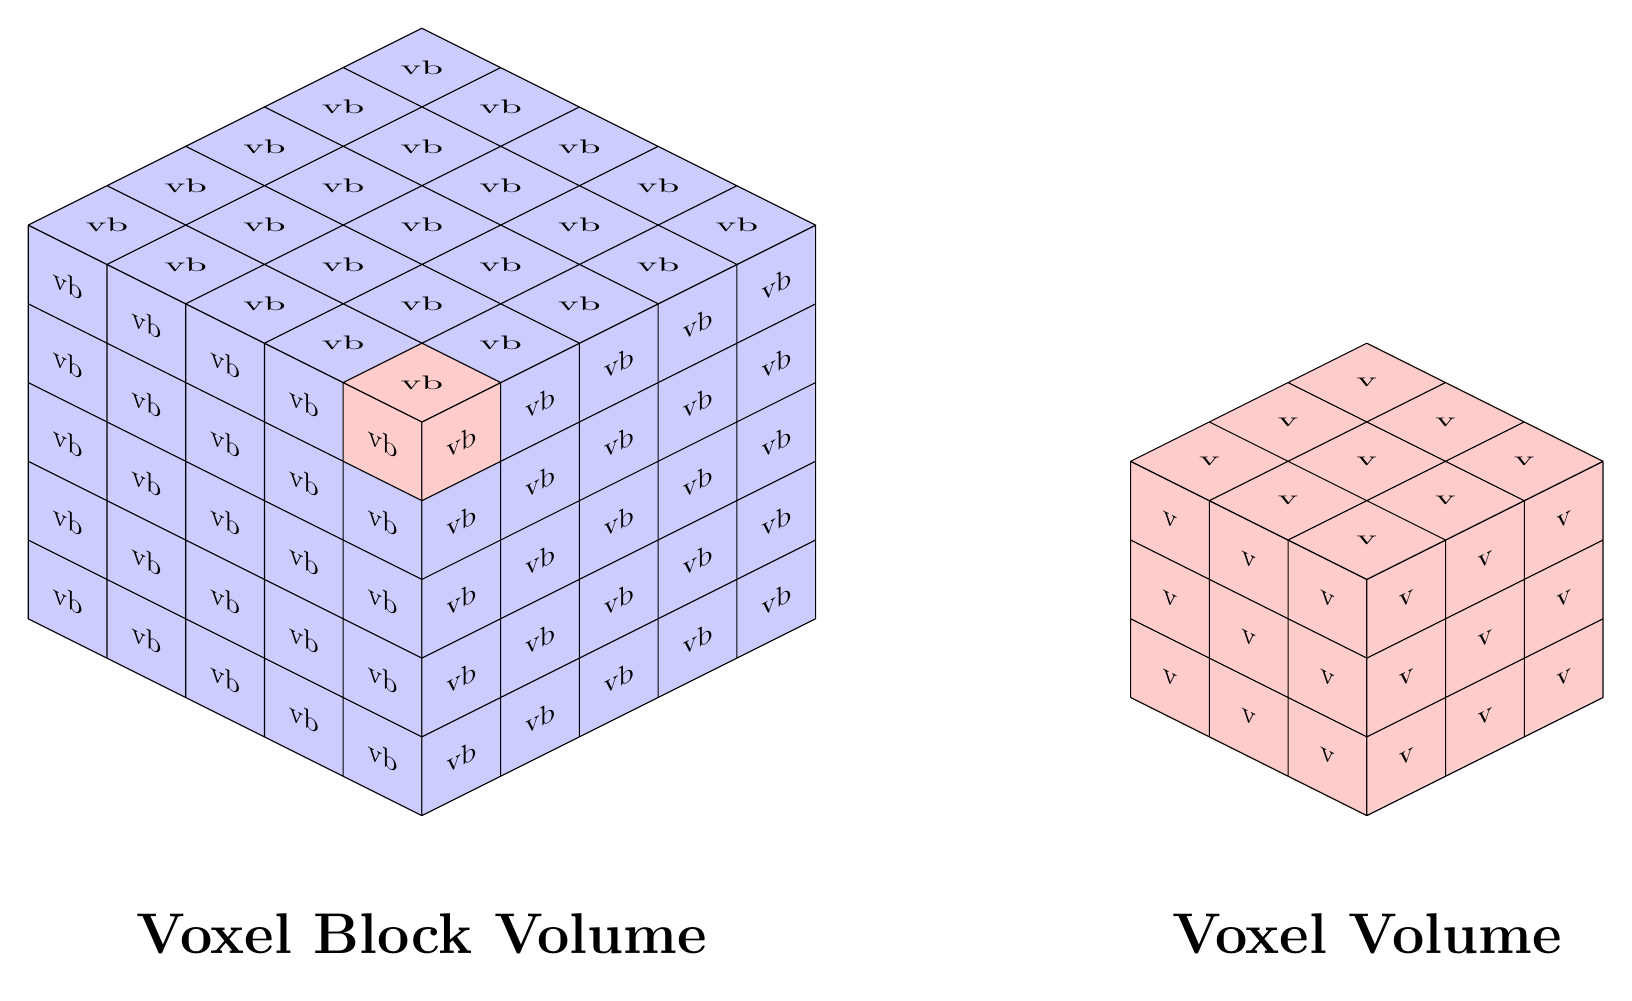
\begin{tikzpicture}[every node/.style={minimum size=1cm},on grid]
      %%%%%%%%%%%%%%%%%%%%%%%%%%%%%%%%%%%%%%%%%%%%%%%%%%%%%%%%%%%%%%%%%%%%%%%%%%
      %%% BEGIN: BIG GRID.
      %%%%%%%%%%%%%%%%%%%%%%%%%%%%%%%%%%%%%%%%%%%%%%%%%%%%%%%%%%%%%%%%%%%%%%%%%%
      % Left face nodes.
      \begin{scope}[every node/.append style={yslant=-0.5},yslant=-0.5]
        \foreach \i in {0,...,4}{
          \foreach \j in {0,...,4}{
            \ifthenelse{\i=4 \AND \j=4}{
              \node[fill=red!20] at (\i+0.5, \j+0.5) {vb};
            }{
              \node[fill=blue!20] at (\i+0.5, \j+0.5) {vb};
            }
          }
        }
        \draw (0,0) grid (5,5);
      \end{scope}

      % Right face nodes.
      \begin{scope}[every node/.append style={yslant=0.5},yslant=0.5]
        \foreach \i in {0,...,4}{
          \foreach \j in {0,...,4}{
            \ifthenelse{\i=0 \AND \j=0}{
              \node[fill=red!20] at (\i+5.5, -1*\j-0.5) {vb};
            }{
              \node[fill=blue!20] at (\i+5.5, -1*\j-0.5) {vb};
            }
          }
        }
        \draw(5, -5) grid (10, 0);
      \end{scope}

      % Top face nodes.
      \begin{scope}[every node/.append style={yslant=0.5,xslant=-1},yslant=0.5,xslant=-1]
        \foreach \i in {0,...,4}{
          \foreach \j in {4,...,0}{
            \ifthenelse{\i=0 \AND \j=0}{
              \node[fill=red!20] at (\i+5.5, \j+0.5) {\rotatebox{-45}{vb}};
            }{
              \node[fill=blue!20] at (\i+5.5, \j+0.5) {\rotatebox{-45}{vb}};
            }
          }
        }
        \draw (5,0) grid (10,5);
      \end{scope}
      \node at (5,-4) {\huge \textbf{Voxel Block Volume}};
      %%%%%%%%%%%%%%%%%%%%%%%%%%%%%%%%%%%%%%%%%%%%%%%%%%%%%%%%%%%%%%%%%%%%%%%%%%
      %%% END: BIG GRID.
      %%%%%%%%%%%%%%%%%%%%%%%%%%%%%%%%%%%%%%%%%%%%%%%%%%%%%%%%%%%%%%%%%%%%%%%%%%

      %%%%%%%%%%%%%%%%%%%%%%%%%%%%%%%%%%%%%%%%%%%%%%%%%%%%%%%%%%%%%%%%%%%%%%%%%%
      %%% BEGIN: SMALL GRID.
      %%%%%%%%%%%%%%%%%%%%%%%%%%%%%%%%%%%%%%%%%%%%%%%%%%%%%%%%%%%%%%%%%%%%%%%%%%
      \begin{scope}[shift={(14,-1)}]
        % Left face nodes.
        \begin{scope}[every node/.append style={yslant=-0.5},yslant=-0.5]
          \foreach \i in {0,...,2}{
            \foreach \j in {0,...,2}{
              \node[fill=red!20] at (\i+0.5, \j+0.5) {v};
            }
          }
          \draw (0,0) grid (3,3);
        \end{scope}

        % Right face nodes.
        \begin{scope}[every node/.append style={yslant=0.5},yslant=0.5]
          \foreach \i in {0,...,2}{
            \foreach \j in {0,...,2}{
              \node[fill=red!20] at (\i+3.5, -1*\j-0.5) {v};
            }
          }
          \draw(3, -3) grid (6, 0);
        \end{scope}

        % Top face nodes.
        \begin{scope}[every node/.append style={yslant=0.5,xslant=-1},yslant=0.5,xslant=-1]
          \foreach \i in {0,...,2}{
            \foreach \j in {2,...,0}{
              \node[fill=red!20] at (\i+3.5, \j+0.5) {\rotatebox{-45}{v}};
            }
          }
          \draw (3,0) grid (6,3);
        \end{scope}
        \node at (3,-3) {\huge \textbf{Voxel Volume}};
      \end{scope}
      %%%%%%%%%%%%%%%%%%%%%%%%%%%%%%%%%%%%%%%%%%%%%%%%%%%%%%%%%%%%%%%%%%%%%%%%%%
      %%% END: SMALL GRID.
      %%%%%%%%%%%%%%%%%%%%%%%%%%%%%%%%%%%%%%%%%%%%%%%%%%%%%%%%%%%%%%%%%%%%%%%%%%
    \end{tikzpicture}
  }
  \caption[TSDF split in to voxel blocks]{A graphical representation of an 
  SDF/TSDF with it's voxels subdivided into voxel blocks. In the above, \(v\) 
  represents voxel blocks and \(v\) voxels.}
~\label{figure:voxel_blocks}
\end{figure}

The remainder of this chapter is structured as follows.
Section~\ref{sec:moseg_related_work} presents an assessment of related and
relevant literature. Section~\ref{sec:moseg_static_fusion} introduces
preliminaries pertaining to the static Fusion pipeline followed by Section
~\ref{sec:moseg_dynamic_fusion} describing the dynamic Fusion component of the
pipeline. Qualitative and quantitative results are presented in Sections
~\ref{sec:moseg_qualitative} and~\ref{sec:moseg_quantitative}, respectively.
Finally, an application to interactive object recognition is given in Section
~\ref{sec:moseg_semantic}.

\section{Static Volumetric Fusion}
~\label{sec:moseg_static_fusion}
The volumetric fusion approach taken in this work draws on previous Volumetric
integration techniques~\cite{Curless1996, Newcombe2011, NieBner2013, Prisacariu2014} 
and shall be introduced in this section as preliminary material as it shall be
referred to in later chapters. Following this approach, at each frame the camera
is tracked against the current scene, after which new data is fused into the
scene model which is then rendered using Raycasting to prepare for tracking in
the next frame.

The static Fusion pipeline consists of the following three consecutive steps:
\begin{itemize}
  \item Camera Tracking.
  \item Model Integration.
  \item Rendering.
\end{itemize}

The approach in this work utilises the TSDF Volumetric data structure which
encodes for each voxel in the structure, a signed value and a weight.
In the case of 3D environment modelling, the values pertain to distances from
surfaces, within some truncation region.

Given a vertex map generated from the back projection of the points in a depth
image, the vertices pertain to the zero crossing point with voxels either side
representing distances to the zero crossing point; positive in front of the
surface, negative behind. Surface points are known as the Zero Level Set.
\begin{figure}[!htbp]
  \centering
  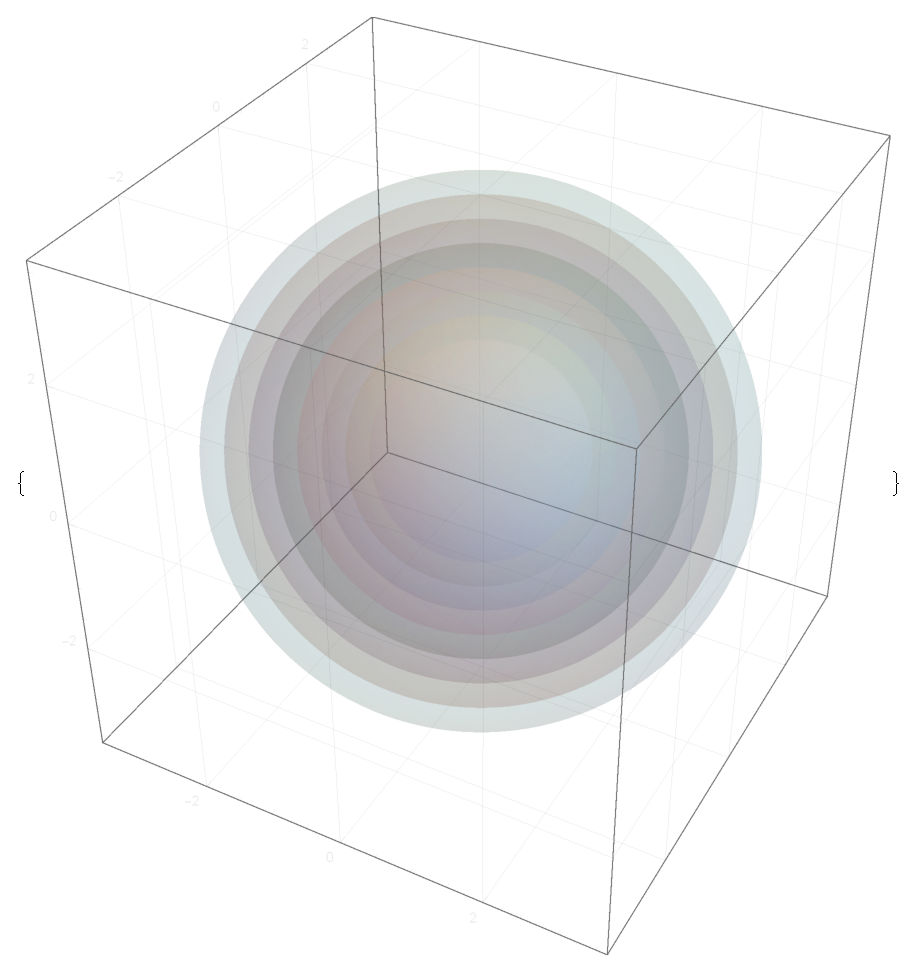
\includegraphics[width=.5\linewidth]{figures/moseg/3d_sdf.eps}
  \caption[Signed Distance Function]{An example of a sphere embedded within a 
  three dimensional SDF.}
~\label{figure:sdf_example}
\end{figure}

For a given TSDF \(\bm{\Phi}\), the Zero Level Set is defined as follows
\begin{equation}
  \label{eqn:zero_level_definition}
  \mathcal{S} = \{v \given \bm{\Phi}(v) = 0\}, 
  \mkern2mu \forall \mkern2mu v \in \bm{\Phi}
\end{equation}
where \(v\) denotes a TSDF voxel. An example of such an embedding is given in
Figure~\ref{figure:sdf_example}.

To facilitate real time fusion, the InfiniTAM framework employs a voxel block
hashing mechanism for fast access to scene voxels~\cite{NieBner2013}. Within
this context, voxel blocks are collections of \(\mathbb{R}^{N \times N \times N}\) 
TSDF voxels, stored in a hash table for fast access. As such, each hash table entry 
corresponds to a portion of a global voxel block array, pertaining to a region in the 
scene. This division of the scene into voxel blocks is used for the later process of 
determining and labelling dynamic regions in the scene.

\subsection{Camera Tracking}
~\label{subsec:moseg_static_camera_tracking}
As in previous works~\cite{Newcombe2011, Prisacariu2014}, the gradient
optimisation based ICP algorithm is utilised to register consecutive images
to derive the camera pose at time \(t\) with respect to time \(t-1\), that is to
optimise for the rigid body transform \(\bm{T} \in \mathbb{SE}(3)\) of the
camera between the two frames using the Levenberg-Marquardt nonlinear least
squares method~\cite{NumericalRecipes}. The rendering stage of the pipeline
is used to generate the image from the TSDF at time \(t-1\) to which a new frame
at time \(t\) is registered.

The target transformation \(\bm{T} \in \mathbb{SE}(3)\) is a member of the
Special Euclidean Group
\begin{equation}
  \label{eqn:se3_definition}
  \mathbb{SE}(3) = \{\bm{R}, \bm{t} \given \bm{R} \in
  \mathbb{SO}(3), \bm{t} \in \mathbb{R}^{3}\}
\end{equation}
and has the following form
\begin{equation}
  \label{eqn:trans_mat_definition}
  \bm{T} =
  \begin{bmatrix}
    \bm{R} & \bm{t} \\
    \bm{0} & 1
  \end{bmatrix}
\end{equation}
where \(\mathbb{SO}(3)\) is the Special Orthogonal Group of Skew Symmetric
Rotation Matrices.

\subsubsection{Attitude Representation}
~\label{subsub:moseg_static_camera_attitude}
The rotation matrix component of the transformation \(\bm{T}\) is
generated by a Rodriguez paramaterization~\cite{Shuster1993}, whereby the
\(\mathbb{SO}(3)\) rotation matrix \(\bm{R}\) is generated by three rotational
parameters, \( \alpha \), \( \beta \) and \( \gamma \). Each parameter represents a 
rotation around one of three principal axes, as shown in Figure~\ref{figure:euler_axes}.
\begin{figure}[!htbp]
  \centering
  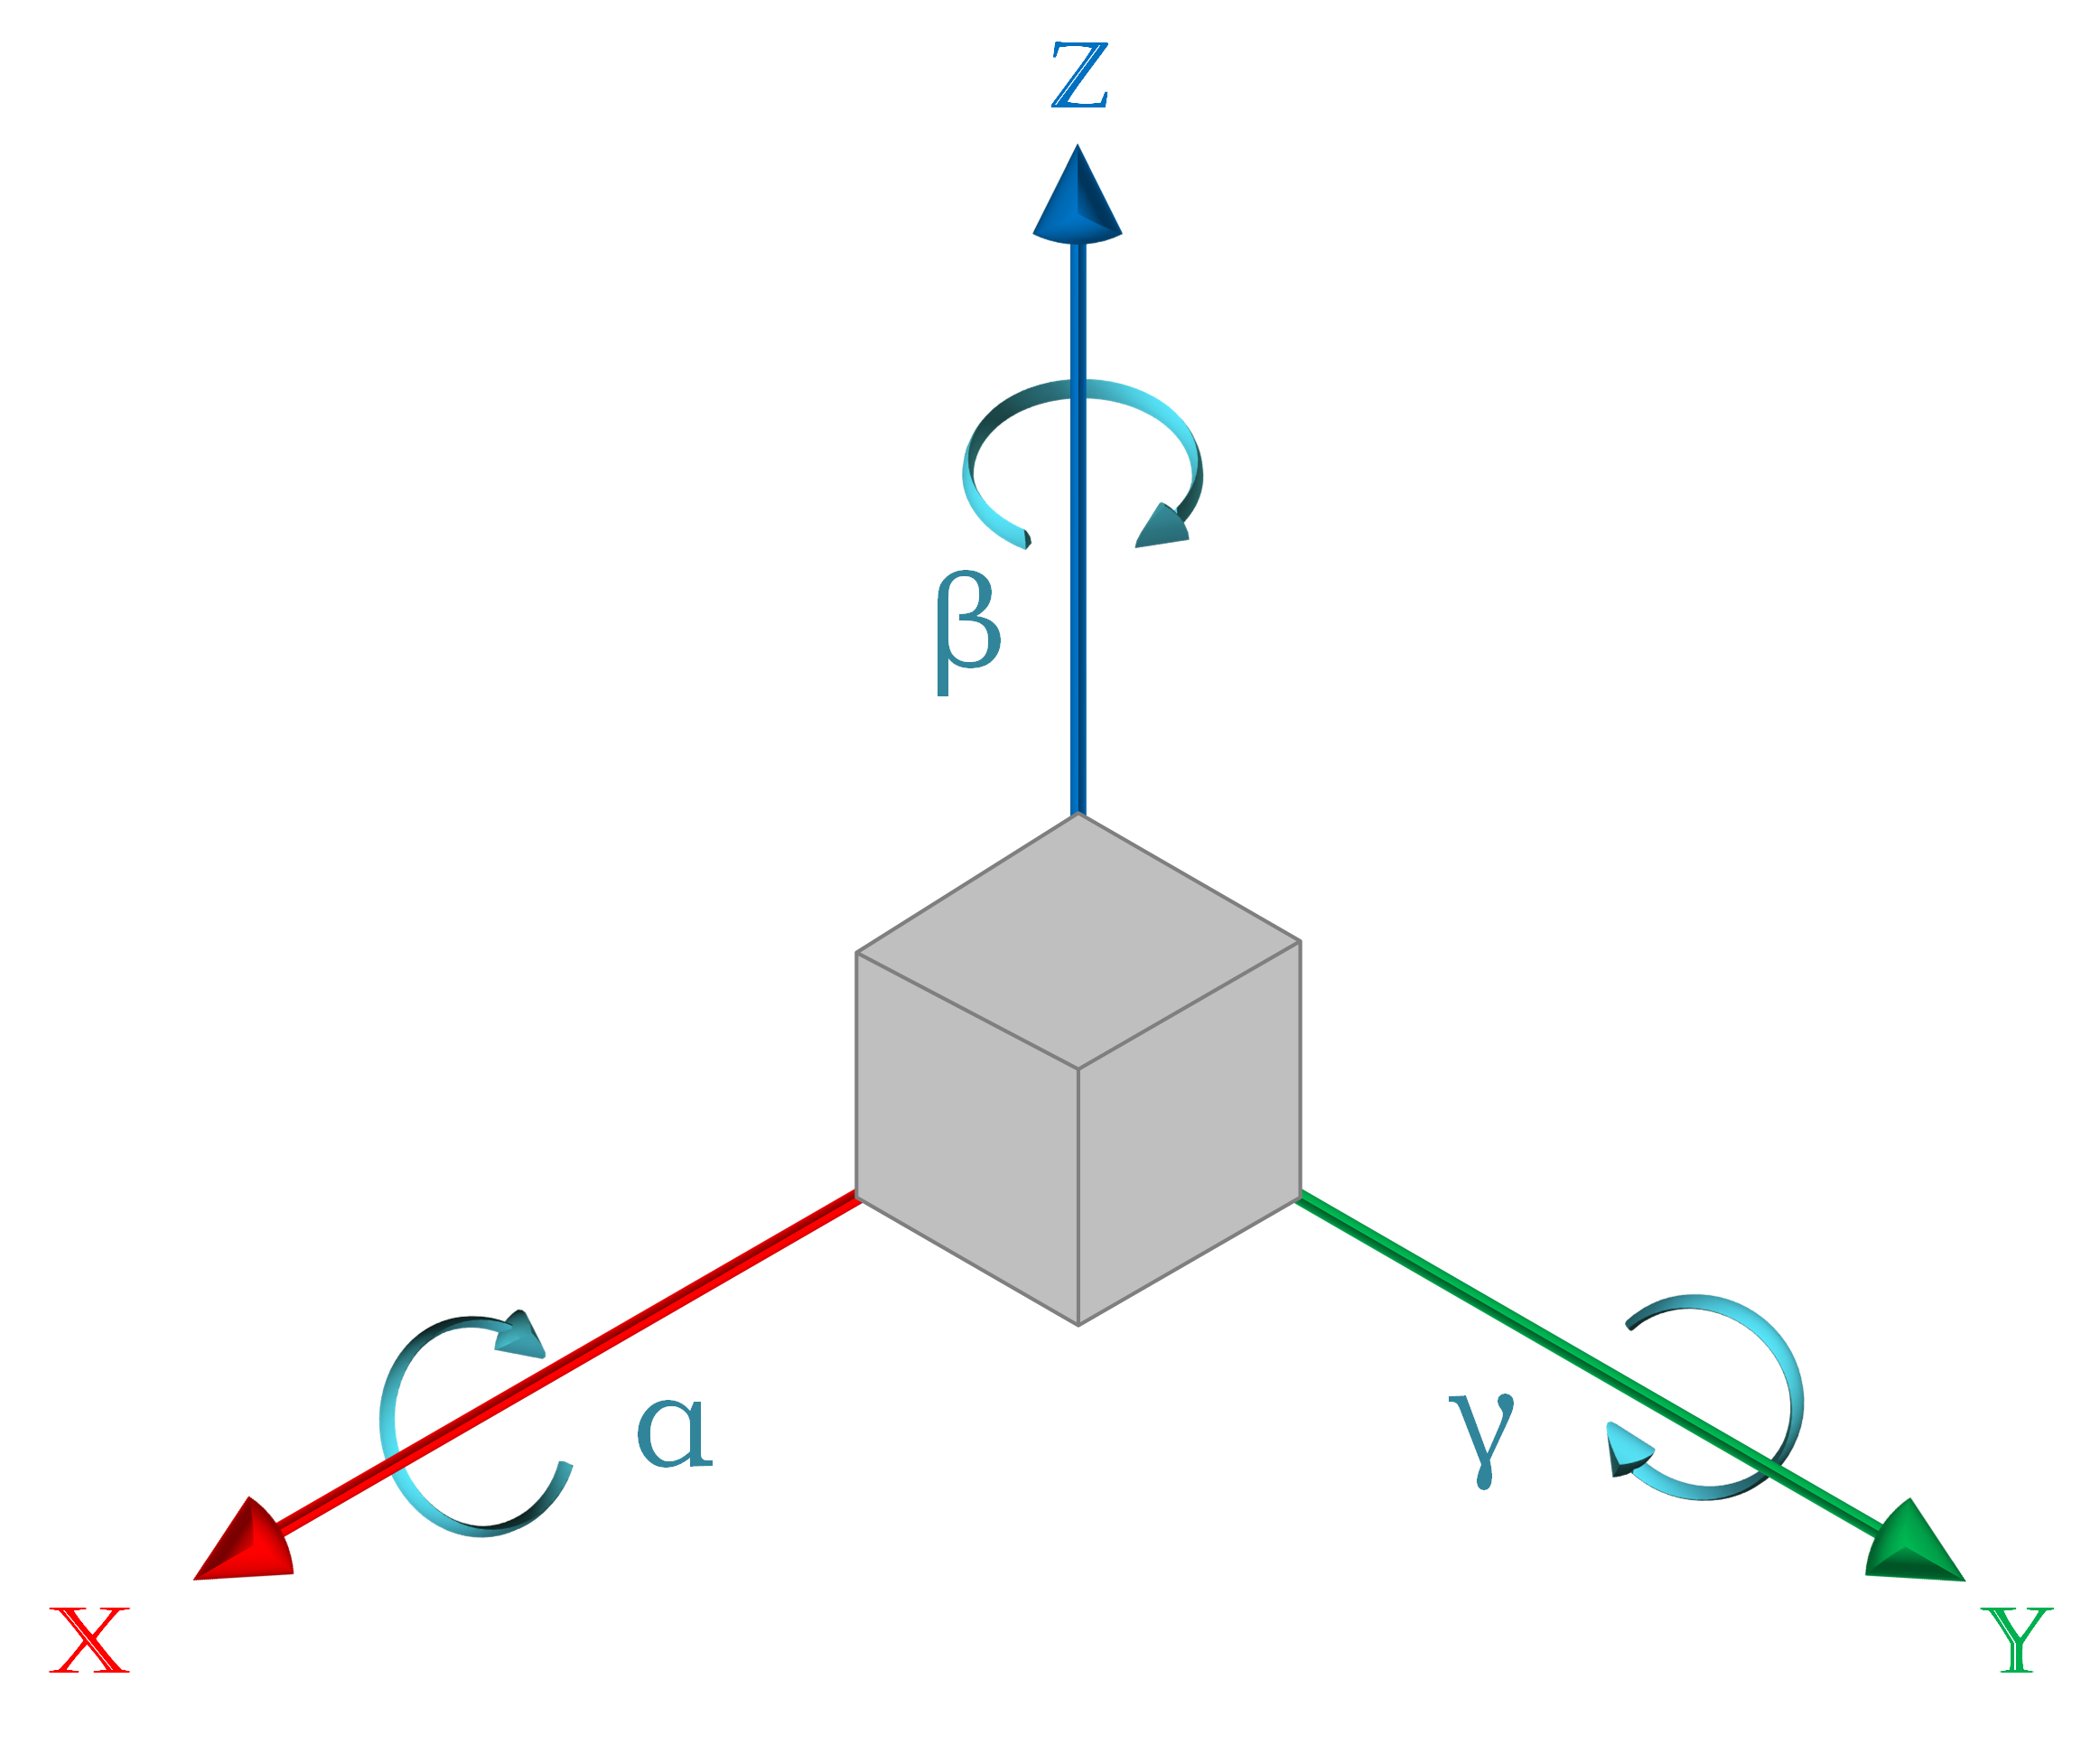
\includegraphics[width=.5\linewidth]{figures/moseg/euler_angles.png}
  \caption[Rotational Axes]{Right handed coordinate system and the three rotational axes; 
  \( \alpha \), \( \beta \) and \( \gamma \).}
~\label{figure:euler_axes}
\end{figure}
The Rodriguez parameters \( \alpha \), \( \beta \) and \( \gamma \) form a member of the Lie Algebra 
\( \mathfrak{g} \) corresponding to the tangent space of the \( \mathbb{SO}(3) \) Lie Group. Elements 
of the Lie Algebra map to the Lie Group by the matrix exponential.

The formulation of the Rodriguez paramaterization (performing the aforementioned matrix exponential)
~\cite{Shuster1993} is given by Equation~\ref{eqn:rodriguez_matrix_eq}, with the parameter vector
\(\bm{p} = {[\alpha, \beta, \gamma]}^{T}\)
\begin{equation}
  \label{eqn:rodriguez_matrix_eq}
  \bm{R}(\bm{p}) =
  \frac{1}{\norm{\bm{p}}^{2}}
  \bigg[
  (1 - \norm{\bm{p}}^{2})\bm{I} +
  2 \bm{pp}^{T} + \omega(\bm{p})
  \bigg]
\end{equation}

Where for an arbitrary vector \(\bm{v}\), \(\omega(\bm{v})\) is defined as
the cross product matrix operator and is defined as follows in Equation~\ref{eqn:cross_prod_mat}.
\begin{equation}
  \label{eqn:cross_prod_mat}
  \omega(\bm{v}) =
  \begin{bmatrix}
    0 & v_{3} & -v_{2} \\
    -v_{3} & 0 & v_{1} \\
    v_{2} & -v_{1} & 0
  \end{bmatrix}
\end{equation}

Evaluating Equation~\ref{eqn:rodriguez_matrix_eq} leads to the following form
of the rotation matrix \(\bm{R}\)
\begin{equation}
  \label{eqn:rodriguez_matrix}
  \bm{R} = \frac{1}{\norm{\bm{p}}^{2} + 1}
  \begin{bmatrix}
    % Row 1.
    \alpha^{2} - \beta^{2} - \gamma^{2} + 1 &
    2 \alpha \beta + \gamma &
    2 \alpha \gamma - \beta \\
    % Row 2.
    2 \alpha \beta - \gamma &
    -(\alpha^{2} - \beta^{2} + \gamma^{2} - 1) &
    \alpha + 2 \beta \gamma \\
    % Row 3.
    2 \alpha \gamma + \beta &
    -(\alpha - 2 \beta \gamma) &
    -(\alpha^{2} + \beta^{2} - \gamma^{2} - 1)
  \end{bmatrix}
\end{equation}

The translational component \(\bm{t}\) of the transformation \(\bm{T}\) is
given by the following vector, with each component representing a translation
along it's respective axis.
\begin{equation}
  \label{eqn:trans_vector}
  \bm{t} =
  \begin{bmatrix}
    t_{x} \\
    t_{y} \\
    t_{z}
  \end{bmatrix}
\end{equation}

\subsubsection{Pose Recovery Formulation}
~\label{subsub:moseg_static_camera_poserec}
The recovery of the camera pose change between frames \(t\) and \(t-1\) may be
formulated as the following point-to-plane energy minimisation problem
\begin{equation}
  \label{eqn:pose_estimation_kf}
  E(\bm{R}, \bm{t}, \bm{\Omega}, \bm{\Phi}) =
  \argmin_{\bm{R}, \bm{t}} \sum_{p \in \bm{\Omega}}
  \norm{{\left[
    \bm{Rx} + \bm{t} - \mathcal{V}(\bar{\bm{x}})
  \right]}^{T}
  \mathcal{N}(\bar{\bm{x}})}
\end{equation}
where in Equation~\ref{eqn:pose_estimation_kf} \(\bm{R}\) and \(\bm{t}\) are 
the aforementioned rotation matrix and translation vector of the transformation 
\(\bm{T}\). \(\bm{x}\) is the 3D point extracted from the depth image 
\(\bm{\Omega}\) and the point \(\bar{\bm{x}}\) is the 3D point in the TSDF 
volume \(\bm{\Phi}\) found by raycasting from \(\bm{\Omega}\) under the 
transformation \(\bm{T}\). Finally, \(\mathcal{N}\) is a normal map of 
\(\bm{\Phi}\) and is defined as follows
\begin{equation}
  \label{eqn:normal_map_definition}
  \mathcal{N} = \frac{\nabla \bm{\Phi}}{\norm{\nabla \bm{\Phi}}}
\end{equation}
where \(\nabla \bm{\Phi}\) is approximated by central finite differencing, 
as follows in Equation~\ref{eqn:sdf_central_diff}.
\begin{equation}
  \label{eqn:sdf_central_diff}
  \nabla \bm{\Phi} = 
    \begin{bmatrix}
      {\big( 2 \delta \bm{v}_{x} \big)}^{-1} \\
      {\big( 2 \delta \bm{v}_{y} \big)}^{-1} \\
      {\big( 2 \delta \bm{v}_{z} \big)}^{-1}
    \end{bmatrix}
    \odot
    \begin{bmatrix}
      \bm{\Phi} \big(\bm{v}_{x} + \delta \bm{v}_{x}\big) - \bm{\Phi} \big(\bm{v}_{x} - \delta \bm{v}_{x}\big) \\
      \bm{\Phi} \big(\bm{v}_{y} + \delta \bm{v}_{y}\big) - \bm{\Phi} \big(\bm{v}_{y} - \delta \bm{v}_{y}\big) \\
      \bm{\Phi} \big(\bm{v}_{z} + \delta \bm{v}_{z}\big) - \bm{\Phi} \big(\bm{v}_{z} - \delta \bm{v}_{z}\big) 
    \end{bmatrix}
\end{equation}

For the gradient update phase of the ICP algorithm, the partial derivatives
\( \frac{\partial E}{\partial \bm{R}_{\lambda}} \forall \lambda \in \{\alpha, \beta, \gamma \} \) 
may be derived as follows in Equation~\ref{eqn:icp_update_derivation_rot}.
As a first step, the following definition is made
\begin{equation}
  \label{eqn:icp_deriv_sub}
  \phi(\bm{R}, \bm{t}, \bm{x}, \bar{\bm{x}}) =
  {\left[
    \bm{Rx} + \bm{t} - \mathcal{V}(\bar{\bm{x}})
  \right]}^{T}
  \mathcal{N}(\bar{\bm{x}})
\end{equation}
With this substitution in place, the derivation proceeds as follows
\begin{align}
  \label{eqn:icp_update_derivation_rot}
  % Line 1.
  \frac{\partial E}{\partial \lambda} ={}&
  \frac{\partial}{\partial \lambda}
  \sum_{p \in \bm{\Omega}}
  \norm{\phi(.)}\\
  % Line 2.
  ={}& \sum_{p \in \bm{\Omega}}
  \frac{\partial}{\partial \lambda}
  \norm{\phi(.)}\\
  % Line 3.
  ={}& \sum_{p \in \bm{\Omega}}
  \frac{\partial}{\partial \phi(.)} \norm{\phi(.)}
  \frac{\partial \phi(.)}{\partial \lambda}\\
  % Line 4.
  ={}& \sum_{p \in \bm{\Omega}}
  \frac{1}{2}{\frac{2 \phi(.)}{\sqrt{\phi(.)}^{T}\phi(.)}}
  \frac{\partial \phi(.)}{\partial \lambda}\\
  % Line 5.
  ={}& \sum_{p \in \bm{\Omega}}
  \frac{\phi(.)}{\norm{\phi(.)}}
  \frac{\partial \phi(.)}{\partial \lambda}\\
  % Line 6
  ={}& \sum_{p \in \bm{\Omega}}
  \frac{\phi(.)}{\norm{\phi(.)}}
  \Bigg[ \frac{\partial}{\partial \lambda}
  {\bigg[ \bm{Rx} + \bm{t} - \mathcal{V}(\bar{\bm{x}}) \bigg]}^{T}
  \mathcal{N}(\bar{\bm{x}}) + 
  {\bigg[ \bm{Rx} + \bm{t} - \mathcal{V}(\bar{\bm{x}}) \bigg]}^{T}
  \frac{\partial}{\partial \lambda}
  \mathcal{N}(\bar{\bm{x}})\Bigg]\\
  % Line 6
  ={}& \sum_{p \in \bm{\Omega}}
  \frac{\phi(.)}{\norm{\phi(.)}}
  {\bigg[ \frac{\partial \bm{R}}{\partial \lambda}
  \bm{x}\bigg]}^{T}
  \mathcal{N}(\bar{\bm{x}})
\end{align}
The full partial derivatives \(\frac{\partial \bm{R}}{\partial \alpha}\),
\(\frac{\partial \bm{R}}{\partial \beta}\) and
\(\frac{\partial \bm{R}}{\partial \gamma}\) may be found Equations
~\ref{eqn:rodrigues_full_alpha_deriv},~\ref{eqn:rodrigues_full_beta_deriv}
and~\ref{eqn:rodrigues_full_gamma_deriv} respectively, of Appendix 
~\ref{appendix:mathematical}.

The partial derivatives
\( \frac{\partial \bm{R}}{\partial \lambda} \forall \lambda \in \{\alpha, \beta, \gamma \} \) 
may be multiplied with \(\bm{x}\) and combined in to the following Rotation Jacobian
\begin{align}
  \label{eqn:rot_jac}
  \bm{J}_{R} ={}& \left. {\bigg[
    \frac{\partial \bm{R}}{\partial \lambda} \bm{x}
    \bigg]}^{T} \right\vert_{\lambda = 0} \\
  ={}&
  \begin{bmatrix}
    0 & -z & y \\
    z & 0 & -x \\
    -y & x & 0
  \end{bmatrix}
\end{align}

Note that the derivation for the partial derivatives
\(\frac{\partial E}{\partial \bm{t}_{\bar{\lambda}}} \forall \bar{\lambda} \in \{x, y, z\} \) 
is analogous with that of Equation~\ref{eqn:icp_update_derivation_rot}, with the result given as 
follows
\begin{equation}
  \label{eqn:icp_update_derivation_trans}
  \frac{\partial E}{\partial \bm{t}_{\bar{\lambda}}} =
  \sum_{p \in \bm{\Omega}}
  \frac{\phi(.)}{\norm{\phi(.)}}
  {\bigg[ \frac{\partial \bm{t}}{\partial \bar{\lambda}}\bigg]}^{T}
  \mathcal{N}(\bar{\bm{x}})
\end{equation}

The translational partial derivatives
\( \frac{\partial \bm{t}}{\partial \lambda} \forall \bar{\lambda} \in \{x, y, z\} \) may also 
be combined in to the following translation Jacobian as in Equation~\ref{eqn:rot_jac}.
\begin{equation}
  \label{eqn:trans_jac}
  \bm{J}_{t} =
  \begin{bmatrix}
    1 & 0 & 0 \\
    0 & 1 & 0 \\
    0 & 0 & 1
  \end{bmatrix}
\end{equation}

The overall combined Jacobian for the energy function defined in Equation
~\ref{eqn:pose_estimation_kf} is as follows
\begin{equation}
  \label{eqn:pose_jacobian}
  \bm{J} =
  \frac{\phi(.)}{\norm{\phi(.)}}
  \begin{bmatrix}
    \bm{J}_{R} & \bm{J}_{t}
  \end{bmatrix}^{T}
  \mathcal{N}(\bar{\bm{x}})
\end{equation}

\subsubsection{Pose Recovery Optimisation}
~\label{subsub:moseg_static_camera_poserec_opt}
With the gradient derivations in place, this section will now detail the
pose recovery procedure. As highlighted, the optimisation routine used is the
Levenberg-Marquardt~\cite{NumericalRecipes} algorithm for solving nonlinear least
squares problems. The gradient update equation for the Levenberg-Marquardt
algorithm is given as follows
\begin{equation}
  \label{eqn:lm_update}
  \theta_{t+1} = \theta_{t} - {(\bm{H} + \lambda \text{diag}(
  \bm{H}))}^{-1}
  \bm{J}
\end{equation}
where \(\theta_{t} = {[\alpha, \beta, \gamma, t_{x}, t_{y}, t_{z}]}^{T}\) is the
parameter vector of \(\bm{T}\) at time \(t\), \(\bm{J}\) is the Jacobian
introduced in Equation~\ref{eqn:pose_jacobian} and \(\bm{H}\) is the Hessian,
approximated by \(\bm{H} = \bm{J}^{T}\bm{J}\). The parameter \( \lambda \)
controls the influence of the gradient on the update step and is adjusted
according to the change in error, as shall be evident in the algorithm
that follows.
{
  \centering
  \singlespacing{}
  \begin{minipage}{.7\linewidth}
    \begin{algorithm}[H]
~\label{alg:icp}
      \caption{ICP with Levenberg-Marquardt}
      \begin{algorithmic}[1]
        % $.$ used instead of \(\) due to a bug(?) in algorithmic.
        \Procedure{ICP}{$\mathcal{D}_{l}, \mathcal{D}_{m}, \mathcal{V}, \theta_{t-1}$}
        \State{\( \lambda \gets \lambda_{init} \)}
        \State{\( \theta_{tmp} \gets \theta_{t-1} \)}
        \State{\( \theta_{t} \gets \theta_{tmp} \)}
        \State{\( \epsilon_{old} \gets \inf \)}
        \State{\( \epsilon \gets \epsilon_{old} \)}
        \While{\( \epsilon >= \tau \)}
        \State{\( \epsilon \gets E(.) \)}
        \Comment{Evaluate Equation~\ref{eqn:pose_estimation_kf}}
        \If{\( \epsilon \leq \epsilon_{old} \)}
        \State{\( \lambda \gets 10\lambda \)}
        \State{\( \theta_{t} \gets \theta_{tmp} \)}
        \Else{}
        \State{\( \lambda \gets \frac{\lambda}{10} \)}
        \State{\( \epsilon_{old} \gets \epsilon \)}
        \State{\( \theta_{tmp} \gets \theta_{t} \)}
        \EndIf{}
        \State{\( \bm{J} \gets \nabla E \)}
        \Comment{Evaluate Equation~\ref{eqn:pose_jacobian}}
        \State{\( \bm{H} = \bm{J}^{T}\bm{J} \)}
        \State{\( \bm{C} = \text{chol}(\bm{H} + \lambda \text{diag}(\bm{H})) \)}
        \State{\( \delta = \text{backsub}(\bm{C}, \bm{J}) \)}
        \State{\( \theta_{tmp} \gets \theta_{tmp} - \delta \)}
        \EndWhile{\\}
        \Return{\( \theta_{t} \)}
        \EndProcedure{}
      \end{algorithmic}
    \end{algorithm}
  \end{minipage}
  \par
}

Note that for numerical stability, the matrix inverse in Equation~\ref{eqn:lm_update} 
may be avoided by utilising the \texttt{chol} and \texttt{backsub} routines to 
compute the Cholesky Decomposition~\cite{NumericalRecipes} and solve a linear system with 
Backsubstitution~\cite{ElemLinAlg}, respectively.

\subsection{Volumetric Integration}
~\label{subsec:moseg_static_integration}
The second phase in the scene reconstruction pipeline is volumetric integration.
That is, the integration of observed depth images into a consistent, implicit
volumetric representation, in this case the existing TSDF model of the scene,
providing the basis for an updated rendering to be used in the ICP procedure
for camera tracking at the next time step.

As previously outlined, the TSDF may be defined as a volume of distances to an
isosurface, with the isosurface itself being given by the Zero Level Set, as
defined in Equation~\ref{eqn:zero_level_definition}. A graphical representation
is given in Figure~\ref{figure:sdf_example}.

As with KinectFusion~\cite{Newcombe2011} the global (scene) location
\(\bm{x}_{v}\) of each voxel \(v \in \bm{\Phi}\) that is visible in the
current view frustum is transformed into the camera's coordinate frame via the
following transformation (noting that \(\bm{x}_{v}\) is in homogeneous form)
\begin{equation}
\label{eqn:project_tsdf_to_image}
\bm{x}_{\Omega} = \bm{K}\bm{T}_i^{-1}\bm{x}_{v}
\end{equation}
where \(\bm{K}\) is the camera's intrinsic calibration matrix, \(\bm{T}\) is
the transformation optimised for at time \(t\), with the form given in Equation
~\ref{eqn:trans_mat_definition} and \(\bm{x}_{\Omega}\) is the resultant
projected coordinates. The form of the camera intrinsic calibration is as 
follows.
\begin{equation}
  \label{eqn:camera_matrix}
  \bm{K} = 
  \begin{bmatrix}
    f_{x} & s & x_{0} & 0\\
    0 & f_{y} & y_{0} & 0\\
    0 & 0 & 1 & 0
  \end{bmatrix}
\end{equation}
Where in Equation~\ref{eqn:camera_matrix}, \(f_{x}\), \(f_{y}\), \(s\), \(x_{0}\) 
and \(y_{0}\) are the focal lengths, scale and camera principal points respectively.

The integration of new data points into the TSDF volume is achieved by computing 
running means; each voxel contains a running average of its SDF value over time.

Projecting to the depth image \(\bm{\Omega}\) coordinates as in Equation
~\ref{eqn:project_tsdf_to_image} to perform a depth pixel lookup in \(\bm{\Omega}\)
and subtracting the \(z\) component of \(\bm{x}_{v}\) from the resulting value
yields the depth offset from the surface, as follows
\begin{equation}
  \label{eqn:integration_offset}
  \eta = \bm{x}_{\Omega} - \bm{x}_{v}^{z}
\end{equation}

If \( \eta \geq -\mu \), that is that the depth of the point is not beyond the
truncation band of the TSDF behind the isosurface, where \( \mu \) is half the 
width of the truncation band, then the TSDF depth measurement update 
proceeds as follows for a voxel \(\bm{x}_{v} \in \bm{\Phi}\).
\begin{equation}
\label{eqn:sdf_update}
\bm{\Phi}{(\bm{x}_{v})}_{t} = \frac{1}{\phi{(\bm{x}_{v})}_{t-1} + 1}
\bigg[\phi{(\bm{x}_{v})}_{t-1}\bm{\bm{\Phi}}{(\bm{x}_{v})}_{t-1} +
\text{min} \bigg( 1, \frac{\eta}{\mu} \bigg)
\bigg]
\end{equation}

\begin{figure}[!htbp]
  \caption{TODO}
~\label{figure:truncation_band}
\end{figure}

In addition, the weight \(\phi(\bm{x}_{v})\) is updated as follows.
\begin{equation}
  \label{eqn:sdf_weight_update}
  \phi{(\bm{x}_{v})}_{t} = \phi{(\bm{x}_{v})}_{t-1} + 1
\end{equation}

\subsection{Rendering}
~\label{subsec:moseg_static_rendering}
Following the integration process outlined in Section ~\ref{subsec:moseg_static_integration} 
is the rendering stage in which an image of the scene under the current pose is generated, to 
provide an updated rendering for the tracking stage outlined in Section~\ref{subsec:moseg_static_camera_tracking}, 
at the next time step.

Rendering in the pipeline is achieved by Raycasting~\cite{Roth1982}, the process of 
``casting'' a ray from the camera frame into the volume representation of the scene, to find intersections with 
the scene isosurface. The basic Raycasting process is Given in Algorithm~\ref{alg:raycast}
{
  \centering
  \singlespacing{}
  \begin{minipage}{\linewidth}
    \begin{algorithm}[H]
~\label{alg:raycast}
      \caption{Volume Raycasting.}
      \begin{algorithmic}[1]
        % $.$ used instead of \(\) due to a bug(?) in algorithmic.
        \Procedure{Raycast}{$\bm{\Phi}, \bm{\Omega}_{in}, \bm{\Omega}_{out}, \bm{C}, \bm{P}, z_{min}, z_{max}, D$}
          \For{\( y \gets 0\ \text{to}\ H \)}
            \For{\( x \gets\ 0\ \text{to}\ W \)}
              % Unproject.
              \State{\( \bm{p}_{min} \gets  \big[
                \frac{x - \bm{C}_{0, 2}}{\bm{C}_{0, 0}}\quad
                \frac{y - \bm{C}_{1, 2}}{\bm{C}_{1, 1}}\quad
                z_{min}\quad 
                1
              \big]^{T} \)} \Comment{Unproject}
              \State{\( \bm{p}_{max} \gets  \big[
                \frac{x - \bm{C}_{0, 2}}{\bm{C}_{0, 0}}\quad
                \frac{y - \bm{C}_{1, 2}}{\bm{C}_{1, 1}}\quad
                z_{max}\quad 
                1
              \big]^{T} \)}
              % Min and max model point.
              \State{\( \bm{p}_{min}^{\star} \gets
                \bm{P}^{-1} \bm{p}_{min}
              \)}\Comment{Object Point}
              \State{\( \bm{p}_{max}^{\star} \gets
                \bm{P}^{-1} \bm{p}_{max}
              \)}
              \State{\( \bm{p}_{min}^{\star} \gets
                D \frac{\bm{p}_{min}^{\star}}{\bm{p}_{min, 3}^{\star}} + \eta
              \)}
              \State{\( \bm{p}_{max}^{\star} \gets
                D \frac{\bm{p}_{max}^{\star}}{\bm{p}_{max, 3}^{\star}} + \eta
              \)}
              % Get step
              \State{\(
                \bm{s} \gets \bm{p}_{max}^{\star} - \bm{p}_{min}^{\star}
              \)}\Comment{Ray Step}
              \State{\(
                \bm{s}^{\star} \gets \frac{\bm{s}}{\lVert \bm{s} \rVert}
              \)}
              % Raycast.
              \State{\( \bm{p}_{m} \gets \bm{p}_{min}^{\star} - \bm{s}^{\star} \)} \Comment{Starting Point}
              \For{\( \delta \gets 0\ \text{to}\ \lVert \bm{s} \rVert \)} \Comment{Traverse the Ray}
                \If{\( \bm{\Phi}(\bm{p}_{m}) \) is valid} \Comment{Write Shaded Pixel}
                  \State{\( \phi \gets \bm{\Phi}(\bm{p}_{m}) \)}
                  \State{\( \bm{x} \gets \bm{P}(\frac{\bm{p}_{m}}{D} - \eta) \)}
                  \State{\( \bm{x}^{\star} \gets \frac{\bm{x}}{\bm{x}_{3}} \)}
                  \State{\( \bm{\Omega}_{x, y} \gets \bm{x}^{\star}_{2} \)}
                  \State{\textbf{break}}
                \EndIf{}
                \State{\( \bm{p}_{m} \gets \bm{p}_{m} + \bm{s}^{\star}\)} \Comment{Increment Model Point}
              \EndFor{}
            \EndFor{}
          \EndFor{}
        \EndProcedure{}
      \end{algorithmic}
    \end{algorithm}
  \end{minipage}
  \par
}

\section{Volumetric Fusion with Dynamic Scenes}
~\label{sec:moseg_dynamic_fusion}
The conventional approach described in Section~\ref{sec:moseg_static_fusion} is adapyted to handle dynamic 
environments. A dual-volume representation of the scene is introduced, consisting of a \emph{static model}
and a \emph{dynamic model} (both of which are TSDF's).

There are two additional stages in the dynamic pipeline to handle integration in
to the static model. The first updates stability values for all of the voxel
blocks in the current view frustum at each frame. The second integrates blocks
whose stability values are above a given threshold into the static model.
Camera tracking is performed against the static model as soon as it contains
valid isosurface data to track against, preventing moving objects in the scene
from contributing to tracking drift.

An overview of the proposed pipeline is given in Figure~\ref{figure:moseg_pipeline}
\begin{figure}[!htbp]
  \centering
  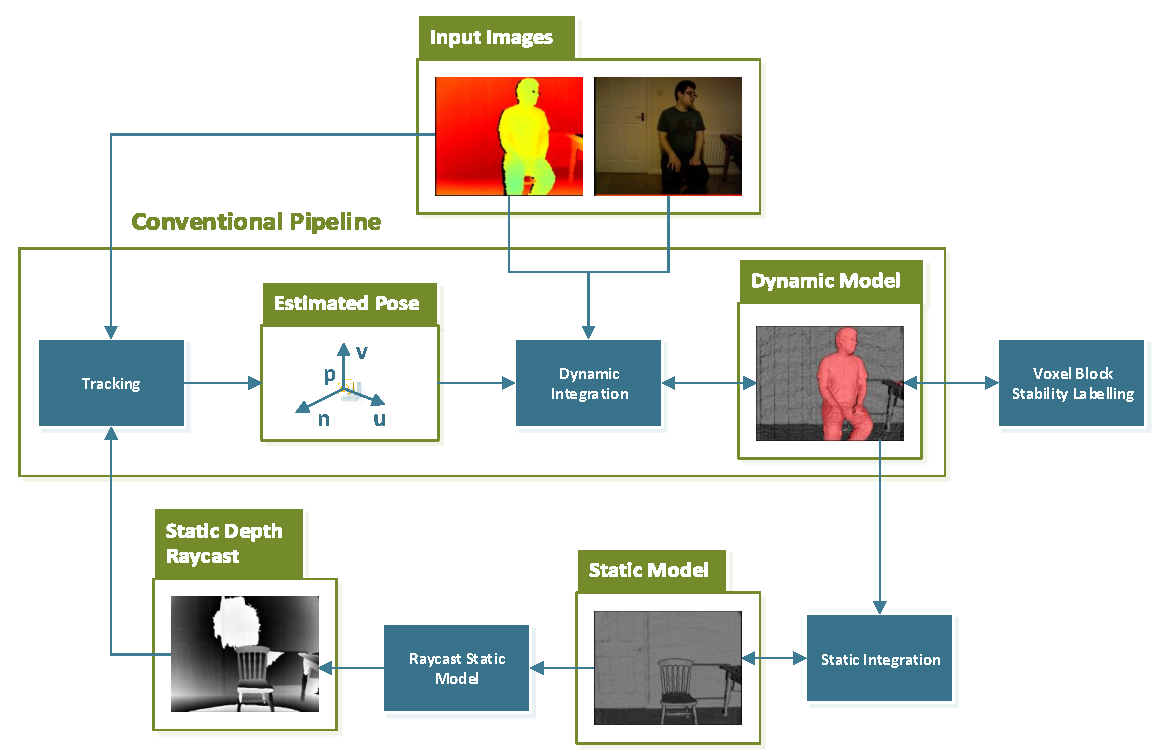
\includegraphics[width=0.95\linewidth]{figures/moseg/pipeline.pdf}
  \caption[Motion Segmentation Pipeline]{The proposed motion segmentation pipeline. 
  Note the additional voxel block labelling stage with a feedback to the model 
  integration stage.}
~\label{figure:moseg_pipeline}
\end{figure}

\subsection{Stability Labelling}
~\label{sub:moseg_stability_labelling}
The purpose of the stability labelling section of the pipeline is to distinguish
between stable and unstable voxel blocks in the dynamic model, resulting in
parts of the scene that are moving being excluded from the static model.

For each voxel block in the dynamic model, a stability value is maintained, 
representing the extent to which the instantaneous TSDF values for the voxels 
in a given voxel block (visible in the current view frustrum under the current 
pose) have remained sufficiently similar to the existing TSDF values for those voxels
over time.

The stability value for each voxel block in the scene is initialised to nought.
At each frame, the instantaneous TSDF values for the voxels in each visible
voxel block are computed. For each voxel block, the mean absolute difference
\( \tau \), between the instantaneous and existing TSDF values is computed as
follows.
\begin{equation}
  \label{eqn:moseg_stability_value}
  \tau_{\mathcal{V}} = \Bigg[ \frac{1}{|\mathcal{V}|} \sum_{v \in \mathcal{V}}
  \bigg|\bm{\Phi}^{d}(v) - \text{min}\bigg(1, \frac{\eta}{\mu}\bigg)\bigg| \Bigg]
\end{equation}
The stability label \( l_{\mathcal{V}} \in \{\text{stable}, \text{unstable}\} \) for
a given voxel block \(\mathcal{V}\) is determined by thresholding on \( \xi \) 
(empirically set to \(0.3m\)) as follows.
\begin{equation}
  \label{eqn:moseg_stability_labelling}
  l_{\mathcal{V}} =
  \begin{cases}
    \text{stable} & \textbf{if} \mkern4mu \tau \leq \xi \\
    \text{unstable} & \textbf{if} \mkern4mu \tau > \xi
  \end{cases}
\end{equation}
If the label \(l_{\mathcal{V}}\) is ``stable'', the implication is that the voxel
block contains few disparities between the current scene and the stored model.
In this case, it's stability value is incremented. If however
\(l_{\mathcal{V}}\) has the label ``unstable'', the implication is that the
contents of the voxel block are changing, so it's stability value is reset to
nought, as follows.
\begin{equation}
  \label{eqn:moseg_stability_update}
  \tau_{\mathcal{V}} =
  \begin{cases}
    \tau_{\mathcal{V}} + 1 & \textbf{if} \mkern4mu l_{\mathcal{V}} =
    \text{stable}\\
    0 & \textbf{if} \mkern4mu l_{\mathcal{V}} = \text{unstable}
  \end{cases}
\end{equation}

Voxel blocks that are observed to be stable over a sufficiently long period of
time (empirically set to \(40\) frames) will be integrated into the static model,
as follows in Section~\ref{sub:moseg_static_to_dynamic}.

\subsection{Integration into Static Model from Dynamic Model}
~\label{sub:moseg_static_to_dynamic}
For a time step \(t\), each voxel block in the dynamic model that has assigned to
it a stable label has the entirety of it's voxel TSDF values integrated into the
static model. In a similar formulation to that given in Equation~\ref{eqn:sdf_update}
of Section~\ref{subsec:moseg_static_integration}, the update comprises 
integration of new data in to a running average.

The weight update for a given voxel \(v\) in the stable model \(\bm{\Phi}^{s}\)
with respect to a voxel (belonging to a voxel block labelled ``stable'') 
\(\bar{v}\) in the dynamic model \(\bm{\Phi}^{d}\) is given as follows.
\begin{equation}
  \label{eqn:moseg_weight_update}
  \phi^{s}_{t}(v) = \phi{(v)}^{s}_{t-1}(v) + \phi{(\bar{v})}^{d}_{t-1}(\bar{v})
\end{equation}
Similarly, the update for the TSDF values is as follows.
\begin{equation}
  \label{eqn:moseg_sdf_update}
  \bm{\Phi}^{s}_{t}(v) = \frac{1}{\phi^{s}_{t}(v)} \bigg[
  \phi^{s}_{t-1}(v) \bm{\Phi}^{s}_{t-1}(v) +
  \phi^{d}_{t-1}(\bar{v}) \bm{\Phi}^{d}_{t-1}(\bar{v})
  \bigg]
\end{equation}

\subsection{Pipeline Summary}
~\label{subsec:moseg_pipeline_summary}
With the central components of the proposed algorithm now outlined, an algorithmic 
summary may be given. As has been highlighted, the central components of the approach 
are the dual volume representation, stability labelling and inter-volume surface 
integration. The process is as follows in Algorithm~\ref{alg:moseg}
{
  \centering
  \singlespacing{}
  \begin{minipage}{\linewidth}
    \begin{algorithm}[H]
~\label{alg:moseg}
      \caption{Motion Segmentation and Dynamic SLAM}
      \begin{algorithmic}[1]
        % $.$ used instead of \(\) due to a bug(?) in algorithmic.
        \Procedure{MoSeg Iteration}{$\bm{\Phi}_{s}, \bm{\Phi}_{d}, \bm{\Omega}, \bm{T}, t$}
          \If{\( t \neq 0 \)}
            \State{\( \mathcal{R} \gets \text{raycast}(\bm{\Phi}_{s}, \bm{\Omega}, \bm{T}) \)}
            \Comment{Section~\ref{subsec:moseg_static_rendering}}
            \State{\( \bm{T}_{t+1} \gets \text{estimatePose}(\mathcal{R}, \mathcal{D}) \)}
            \Comment{Section~\ref{subsec:moseg_static_camera_tracking}}
            \State{\( \text{updatePose}(\bm{T}_{t+1}) \)}
          \EndIf{}

          \State{\( \mathcal{D} \gets \text{unproject}(\bm{\Omega}_{d}) \)}
          \State{\( \bm{\Phi}_{d} \gets \text{integrate}(\mathcal{D}, \bm{\Phi}_{d}, \bm{T})\)}
          \Comment{Equation~\ref{eqn:sdf_update}}

          \For{\( p \in \mathcal{D} \)}
            \State{\( b \gets \text{getVoxelBlock}(p) \)}\\
            \State{\( \tau_{b} \gets \text{getStability}(b) \)}
            \Comment{Equation~\ref{eqn:moseg_stability_value}}
            \State{\( l_{b} \gets \text{getLabel}(\tau_{b}) \)}
            \Comment{Equation~\ref{eqn:moseg_stability_labelling}}
            \State{\( \text{updateStability}(b, l_{b}) \)}
            \Comment{Equation~\ref{eqn:moseg_stability_update}}\\

            \If{\( t \leq \text{initial\_frame\_count} \lor l_{b} == \text{stable} \)}
              \For{\( v \in \text{getVoxels}(b) \)}
                \State{\( \phi_{s}(v) \gets \text{getWeight}(v) \)}
                \State{\( \phi_{d}(v) \gets \text{getWeight}(v) \)}
                \State{\( \bm{\Phi}_{s}(v) \gets \text{integrate}(\bm{\Phi}_{s}(v), 
                \bm{\Phi}_{d}(v)), \phi_{s}(v), \phi_{d}(v) \)}
                \Comment{Equation~\ref{eqn:moseg_sdf_update}}
                \State{\( \text{updateStableWeight}(\phi_{s}(v), \phi_{d}(v)) \)}
                \Comment{Equation~\ref{eqn:moseg_weight_update}}
              \EndFor{}
            \EndIf{}
          \EndFor{}

          \State{\( \text{raycast}(\bm(\Phi)_{d}, \bm{T}) \)}
          \Comment{Visualise Dynamics}
        \EndProcedure{}
      \end{algorithmic}
    \end{algorithm}
  \end{minipage}
  \par
}

\section{Qualitative Results}
~\label{sec:moseg_qualitative}
Empirically, the proposed motion segmentation system is capable of retaining
globally consistent tracking within the dense SLAM framework for a range of
scenarios that would prove to be problematic for other, static dense SLAM
systems. The experiments performed demonstrate a robustness	to dynamics in
various scenes, both in terms of tracking and noise artefacts in the static
model. In addition, the system is robust to the addition and removal of scene
components and is robust to short term occlusions, such as a person walking in
front of the camera. An example of a person moving in to the the view frustrum
and sitting on a Setee is given in Figure~\ref{figure:moseg_qualitative_setee}.

\begin{figure}[!htbp]
  \centering
  \begin{tabular}{ccc}
    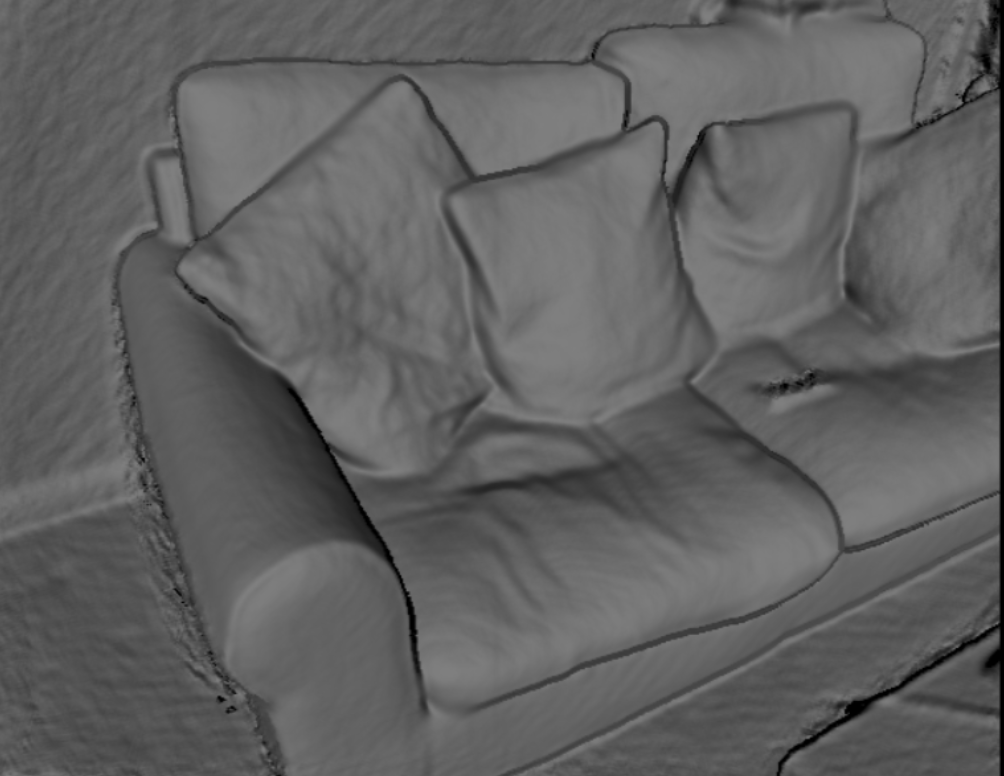
\includegraphics[height=.2\linewidth]{figures/moseg/original_sitting.png} &
    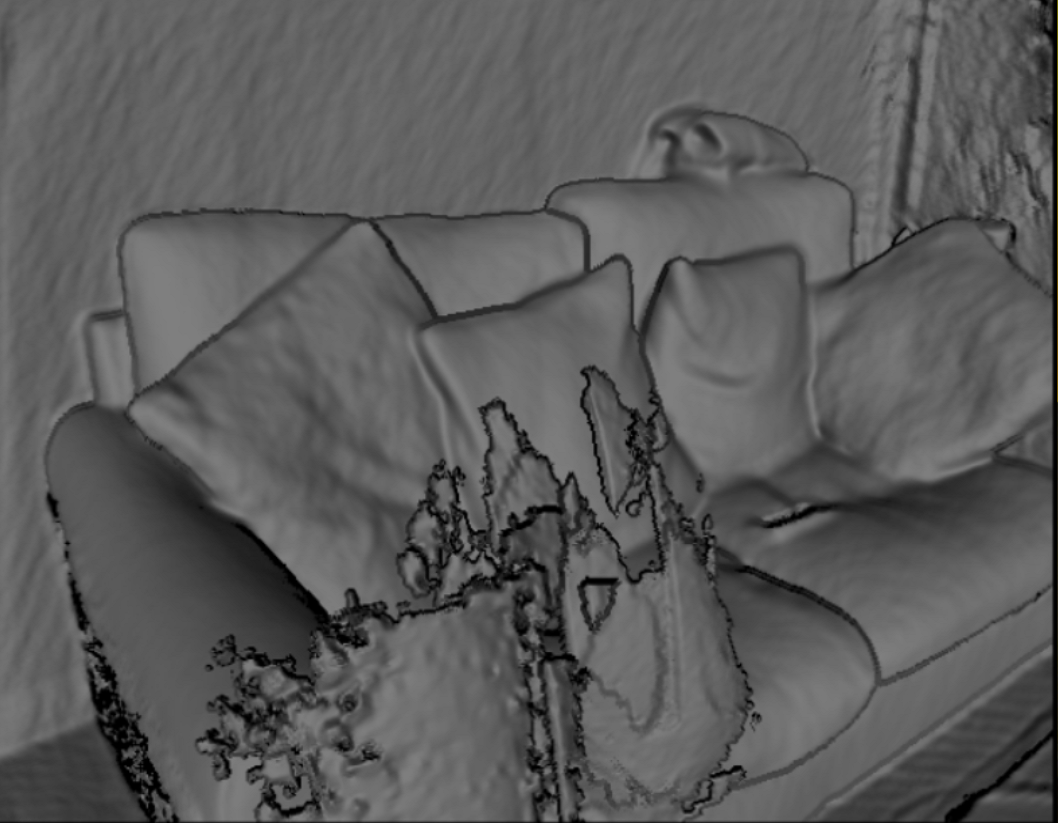
\includegraphics[height=.2\linewidth]{figures/moseg/infinitam_sitting.png} &
    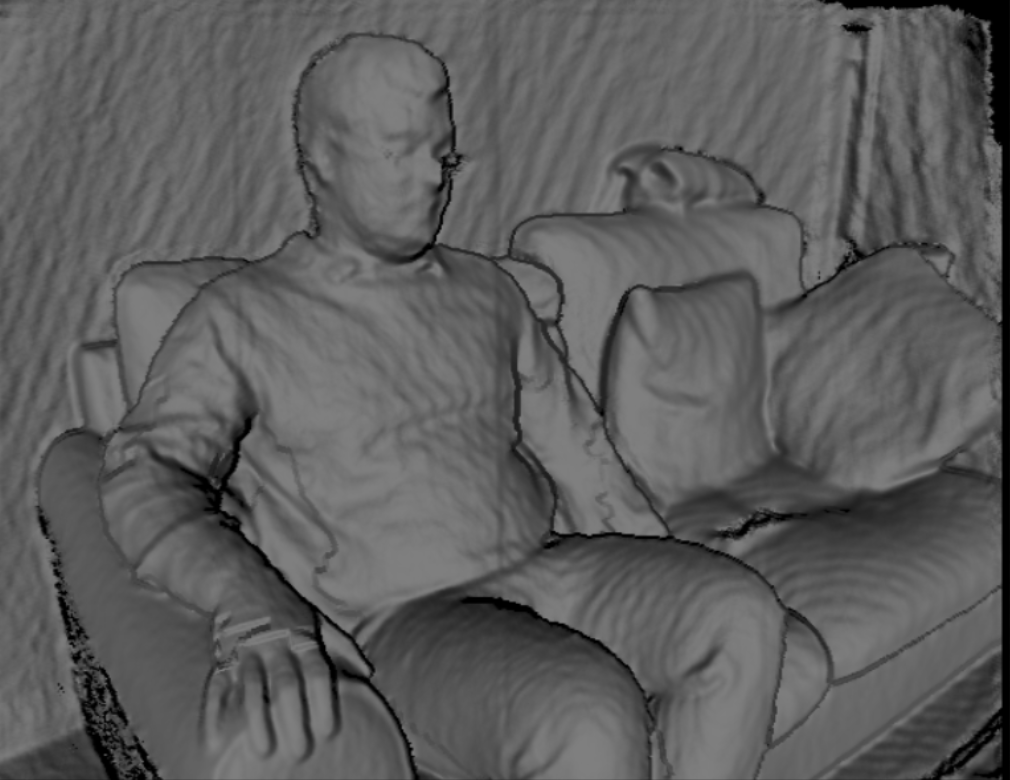
\includegraphics[height=.2\linewidth]{figures/moseg/moseg_sitting.png}\\
    (a) & (b) & (c)
  \end{tabular}
  \caption[Motion Segmentation Qualitative Results I]
  {A qualitative comparison between the proposed system and InfiniTAM~\cite{Prisacariu2014}.
    (a) A static scene containing a Setee is reconstructed.
    (b) When a person enters the scene using standard InfiniTAM, the tracking
    fails, leading to a corrupted scene model.
    (c) Using the proposed system, tracking is maintained and the person is
    integrated successfully into the scene.}
~\label{figure:moseg_qualitative_setee}
\end{figure}

In addition to the ability to reconstruct a moving object that becomes static in
the scene as shown in Figure~\ref{figure:moseg_qualitative_setee}, the proposed
system is also capable of segmenting dynamic objects in a scene that are
undergoing nonrigid motion. Whilst these objects are segmented and labelled as
``dynamic'' they are not used for camera pose estimation. An example of this
behaviour may be observed in Figure~\ref{figure:moseg_qualitative_chair}.

\begin{figure}[!htbp]
  \centering
  \begin{tabular}{cc}
    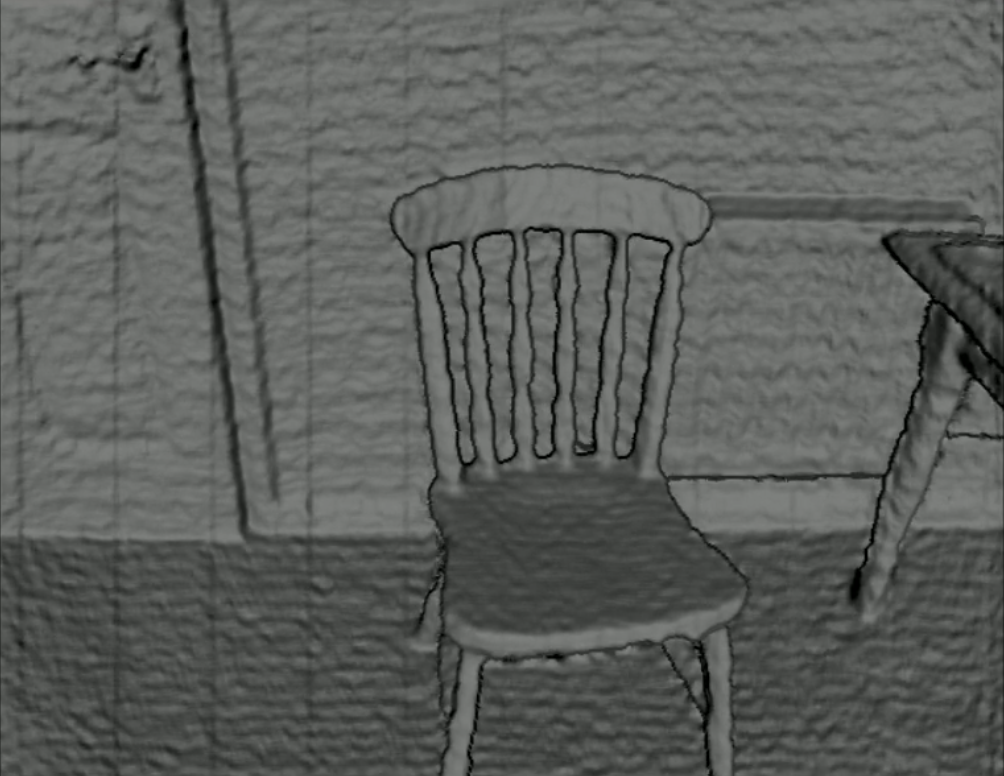
\includegraphics[height=.25\linewidth]{figures/moseg/chair0.png} &
    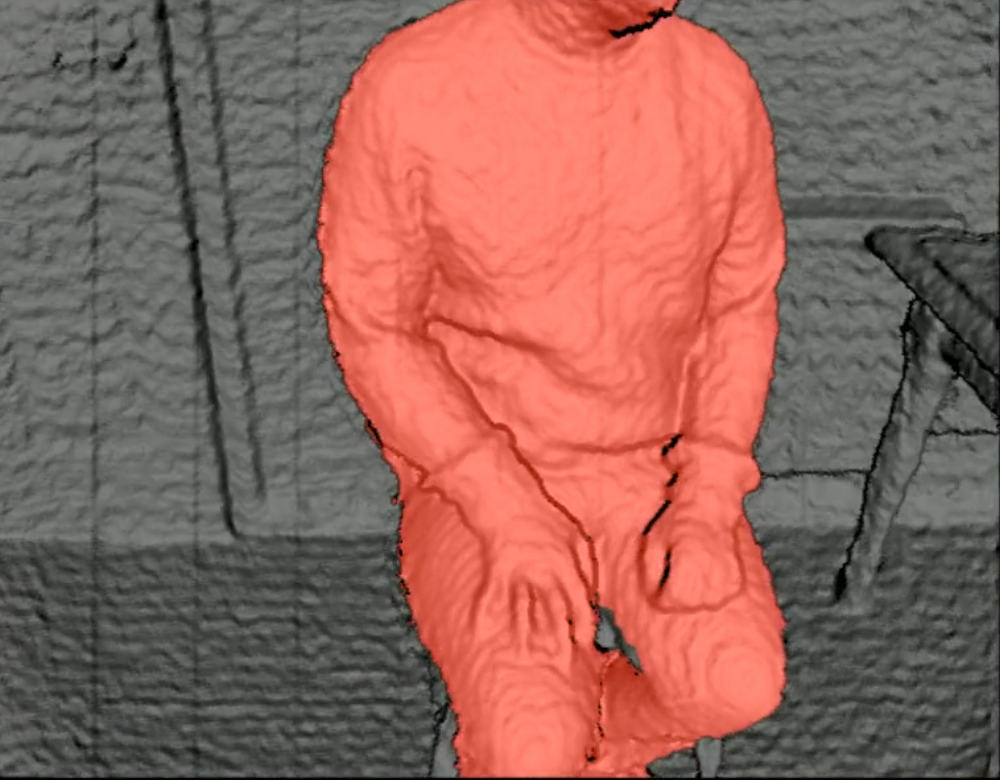
\includegraphics[height=.25\linewidth]{figures/moseg/chair1.png} \\
    (a) & (b) \\
    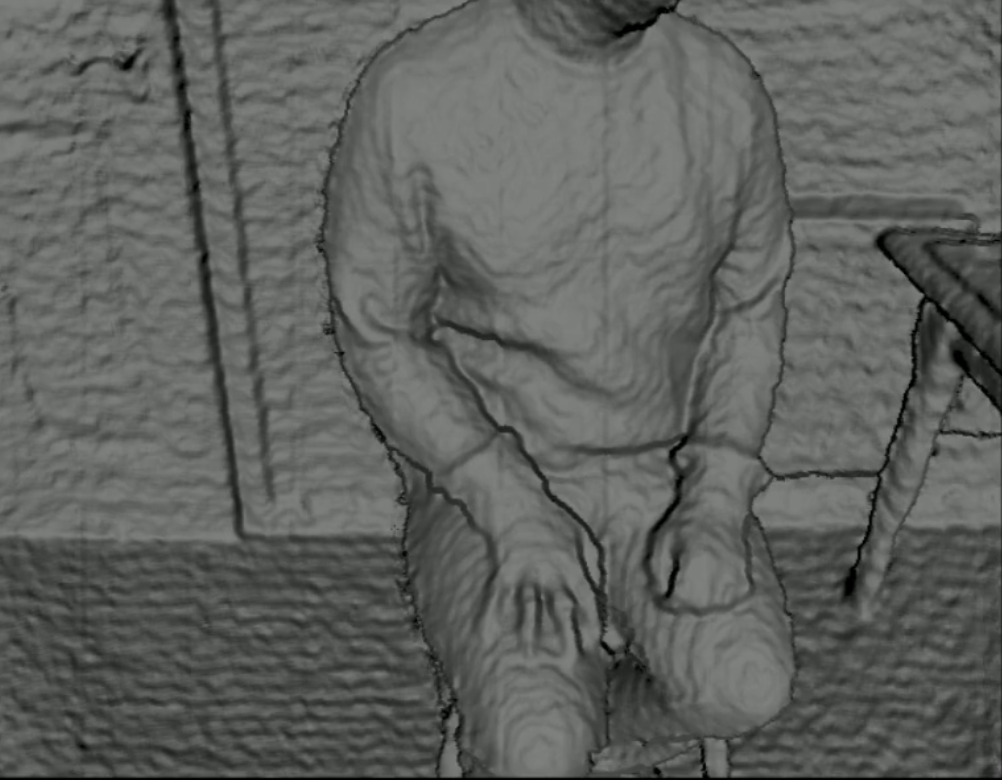
\includegraphics[height=.25\linewidth]{figures/moseg/chair2.png} &
    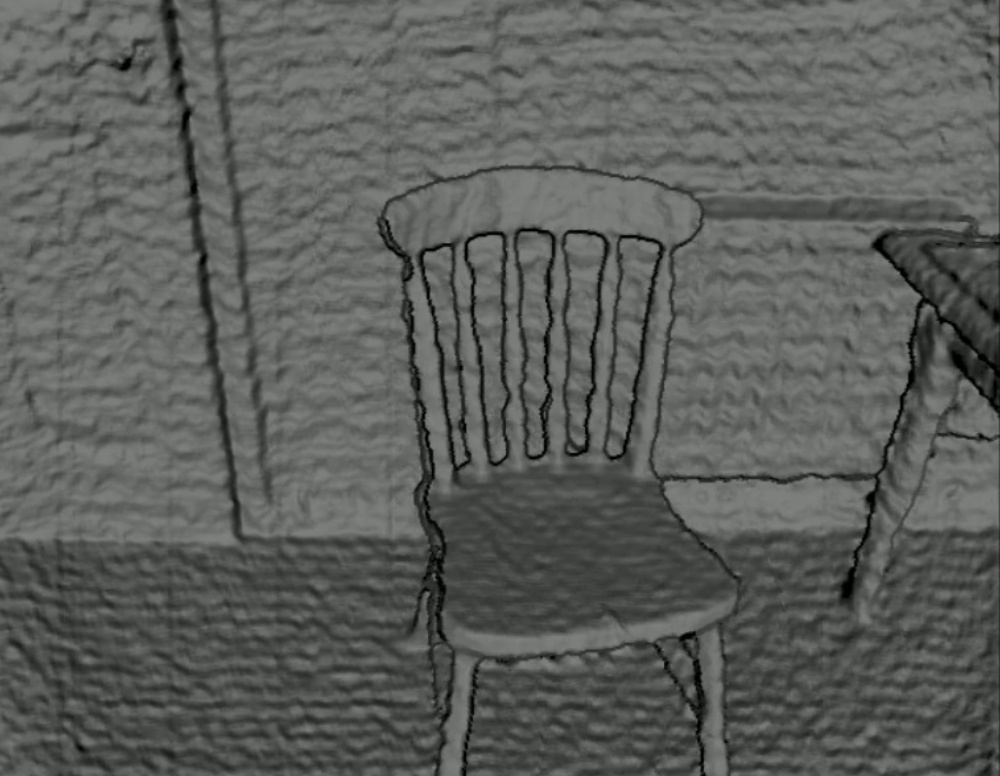
\includegraphics[height=.25\linewidth]{figures/moseg/chair3.png} \\
    (c) & (d)
  \end{tabular}
  \caption[Motion Segmentation Qualitative Results II]
  {A qualitative example of the proposed systems ability to segment
    dynamic scene components.
    (a) A static scene containing a Chair is reconstructed.
    (b) A person enters the scene, is marked as ``dynamic'' and sits down.
    (c) After gaining a sufficient confidence score, the person is labelled
    ``static'' and is integrated in to the static model.
    (d) The person gets up from the Chair and leaves the scene. The original
    reconstruction of the Chair from (a) is in tact.}
~\label{figure:moseg_qualitative_chair}
\end{figure}

\section{Quantitative Results}
~\label{sec:moseg_quantitative}
In this section, a quantitative evaluation of the system's efficacy in terms of
and camera tracking ability is provided.

For the quantitative analysis, the system has been evaluated on the dynamic
objects subset of the TUM RGBD dataset~\cite{Sturm2012} with respect to
trajectory quality. The scenes provided in the dataset contain a range of
dynamic components ranging from arm movement to people walking around, occluding
parts of the scene. Comparison is drawn against the standard InfiniTAM framework
on which the proposed system is based, using standard, static InfiniTAM as a
baseline.

\begin{table}[!htbp]
\begin{center}
  \begin{tabular}{l c c}
    \emph{TUM Standard Sequence Name} & \emph{MoSeg} ATE & \emph{Baseline} ATE \\
    \midrule
    \textsf{fr2-desk-with-person} & \textbf{0.158 \std{0.091}} & 0.297 \std{0.193}\\
    \textsf{fr3-sitting-static} & 0.014 \std{0.008} & \textbf{0.012 \std{0.007}}\\
    \textsf{fr3-sitting-xyz} & 0.064 \std{0.031} & \textbf{0.053 \std{0.029}}\\
    \textsf{fr3-sitting-halfsphere} & 0.142 \std{0.063} & \textbf{0.115 \std{0.049}}\\
    \textsf{fr3-sitting-rpy} & \textbf{0.056 \std{0.033}} & 0.081 \std{0.051}\\
    \textsf{fr3-walking-static} & \textbf{0.294 \std{0.153}} & 0.999 \std{0.178}\\
    \textsf{fr3-walking-xyz} & \textbf{0.385 \std{0.271}} & 0.544 \std{0.343}\\
    \textsf{fr3-walking-halfsphere} & \textbf{0.539 \std{0.360}} & 0.762 \std{0.367}\\
    \textsf{fr3-walking-rpy} & \textbf{0.662 \std{0.335}} & 0.843 \std{0.365}\\
  \end{tabular}
\end{center}
\caption[Motion Segmentation ATE]
{The Absolute Trajectory Error (ATE) results (in metres, lower is better) 
achieved by the proposed approach in comparison to the baseline InfiniTAM
~\cite{Prisacariu2014} framework on a variety of the standard sequences from
  the TUM RGBD dataset~\cite{Sturm2012}. Results are in the format mean
  \( \pm \) standard deviation. The better result (by mean) on each sequence is
  highlighted in bold.}
~\label{table:moseg_ate}
\end{table}

Given in Table~\ref{table:moseg_ate} is the Absolute Trajectory Error measures
for each of the TUM Dynamic Scenes. The Absolute Trajectory Error utilises the
method of Horn~\cite{Horn1987} to solve for the error incurred by mapping the
trajectory of the proposed system on to the ground truth trajectory of the TUM
sequence, for a given TUM Dynamic Objects sequence.

The results of Table~\ref{table:moseg_ate} are visualised in Figure
~\ref{figure:moseg_ate}.

\begin{figure}[!htbp]
  \centering
  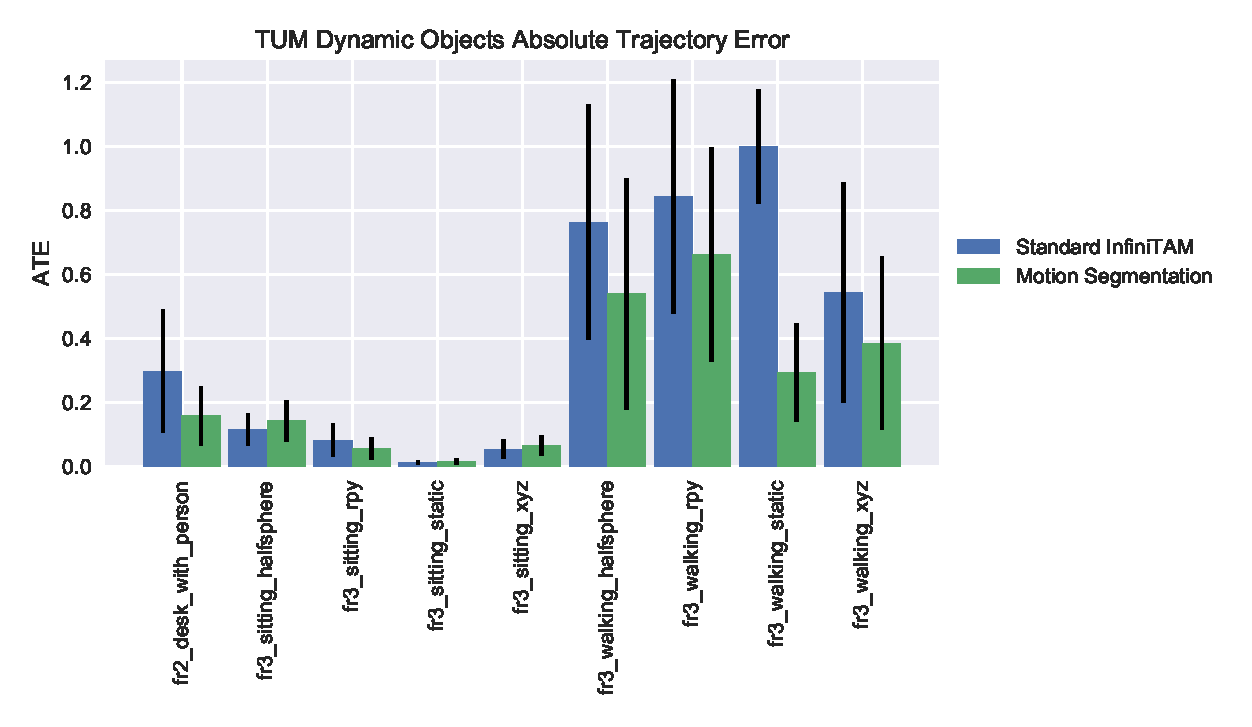
\includegraphics[width=0.95\linewidth]{figures/moseg/ate.eps}
  \caption[Motion Segmentation ATE]
  {Absolute Trajectory Error for the TUM Dynamic Scenes dataset.}
~\label{figure:moseg_ate}
\end{figure}

In addition to evaluating quantitatively in terms of Absolute Trajectory Error,
additional results are provided in terms of Relative Trajectory Error
~\cite{Sturm2012}. RTE measures the relative pose error over a fixed time
interval, with the final score being the Root Mean Squared Error (RMSE) over all 
time windows. RTE results are provided in Table~\ref{table:moseg_rte} and visualised 
in Figure~\ref{figure:moseg_rte}.

\begin{table}[!htbp]
\begin{center}
  \begin{tabular}{l c c}
    \emph{TUM Standard Sequence Name} & \emph{MoSeg} RTE & \emph{Baseline} RTE \\
    \midrule
    \textsf{fr2-desk-with-person} & \textbf{0.023 \std{0.030}} & 0.026 \std{0.037}\\
    \textsf{fr3-sitting-static} & 0.010 \std{0.008} & \textbf{0.010 \std{0.008}}\\
    \textsf{fr3-sitting-xyz} & 0.028 \std{0.017} & \textbf{0.028 \std{0.017}}\\
    \textsf{fr3-sitting-halfsphere} & \textbf{0.031 \std{0.033}} & 0.032 \std{0.029}\\
    \textsf{fr3-sitting-rpy} & 0.073 \std{0.061} & \textbf{0.067 \std{0.065}}\\
    \textsf{fr3-walking-static} & \textbf{0.082 \std{0.140}} & 0.163 \std{0.308}\\
    \textsf{fr3-walking-xyz} & 0.410 \std{0.262} & \textbf{0.300 \std{0.252}}\\
    \textsf{fr3-walking-halfsphere} & \textbf{0.245 \std{0.320}} & 0.305 \std{0.374}\\
    \textsf{fr3-walking-rpy} & 0.482 \std{0.456} & \textbf{0.406 \std{0.364}}\\
  \end{tabular}
\end{center}
\caption[Motion Segmentation RTE]
{The Relative Trajectory Error (RTE) results (in metres, lower is better) 
achieved by the proposed approach in comparison to the baseline InfiniTAM
~\cite{Prisacariu2014} framework on a variety of the standard sequences from
the TUM RGBD dataset~\cite{Sturm2012}. Results are in the format mean
\( \pm \) standard deviation. The better result (by mean) on each sequence is
highlighted in bold.}
~\label{table:moseg_rte}
\end{table}

\begin{figure}[!htbp]
  \centering
  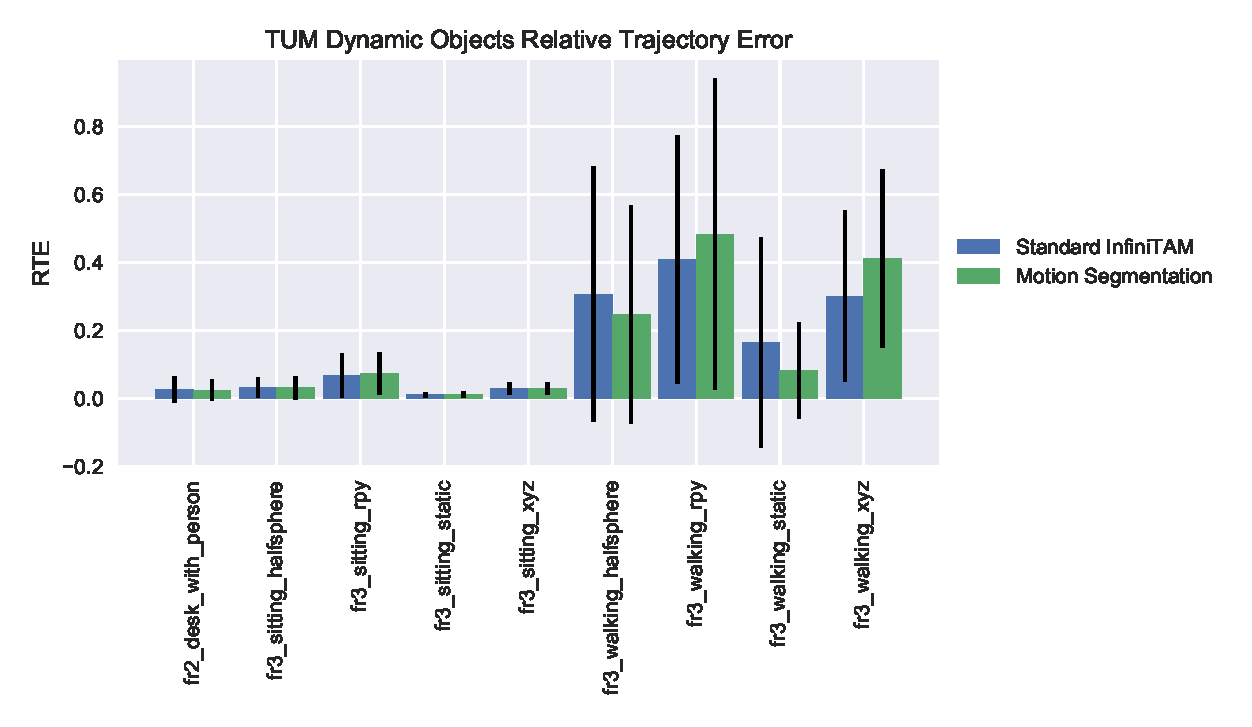
\includegraphics[width=0.95\linewidth]{figures/moseg/rte.eps}
  \caption[Motion Segmentation RTE]
  {Relative Trajectory Error for the TUM Dynamic Scenes dataset.}
~\label{figure:moseg_rte}
\end{figure}

\section{Application to Semantic Scene Understanding}
~\label{sec:moseg_semantic}
The dynamic scene handling approach described in Section~\ref{sec:moseg_dynamic_fusion}
can be used to prevent moving objects from being integrated into the static
scene model. However, for many applications (e.g.\ mobile robotics), there is an
additional need to understand what objects are present in the scene and where
they are, as outlined in Section~\ref{sec:intro_scene_recon}.

In this section, it is therefore shown that classifiers may be trained for the
moving objects and used to recognise new instances of those objects as they
enter the scene.

The voxel blocks in the dynamic model that were identified as ``unstable''
provide a natural representation of the dynamic parts of the scene. Where
multiple dynamic objects are present, they can be separated by finding the
connected components of these voxel blocks. For each object, a one-class Support
Vector Machine (SVM)~\cite{Singer07} with a polynomial kernel is trained and used 
to recognise new instances of the object class.

Upon seeing a new object, the system first tries to classify the object into a category
that has already been seen, by predicting the objects class with all of the existing single class 
SVMs. If this fails, the system generates a label for the object and trains a new SVM for it's 
class. 

To make the training examples for the detected object, points are uniformly sampled from the object's
isosurface and Fast Point Feature Histogram (FPFH) descriptors~\cite{Rusu2009} are computed
at those points. FPFH descriptors are geometric features that provide a
per-point statistic of the curvature within some neighbourhood of the point
(empirically, a \(2.5cm\) radius around the point is used).

Figure~\ref{figure:moseg_recognition} shows an example of this training and
prediction process for dynamic objects.

\begin{figure}[!htbp]
  \centering
  \begin{tabular}{ccc}
    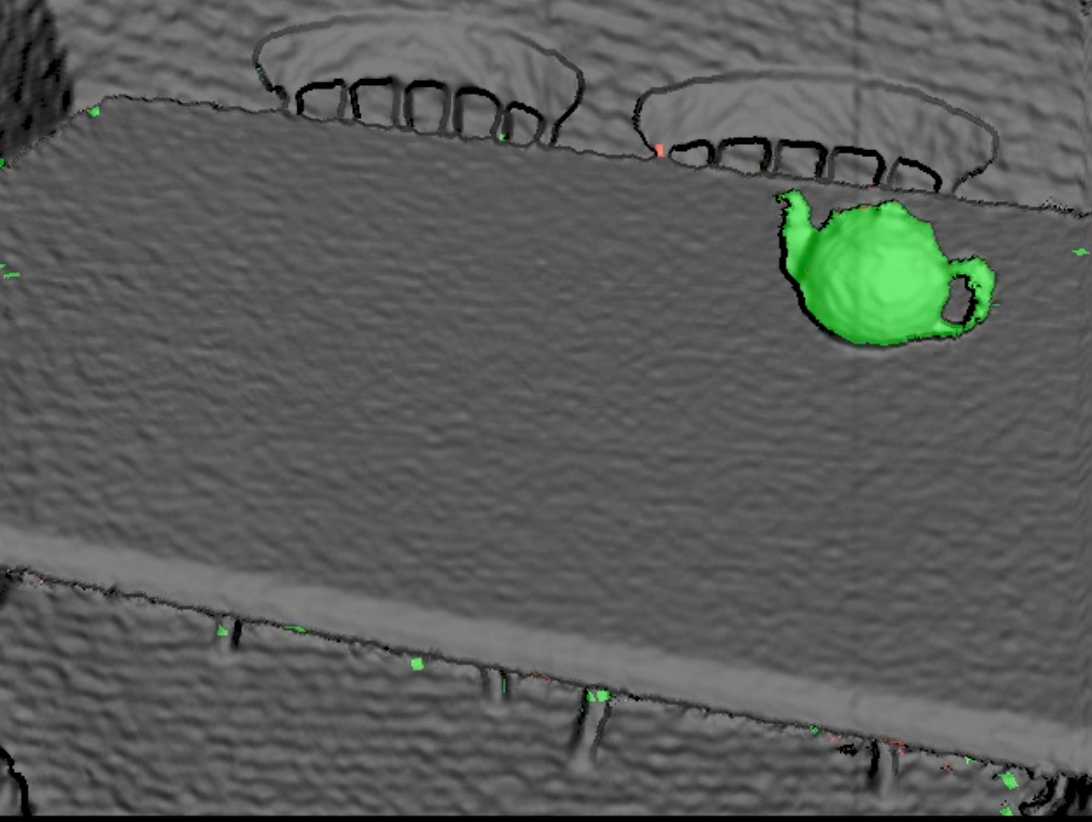
\includegraphics[width=.28\linewidth]{figures/moseg/objects1.png} &
    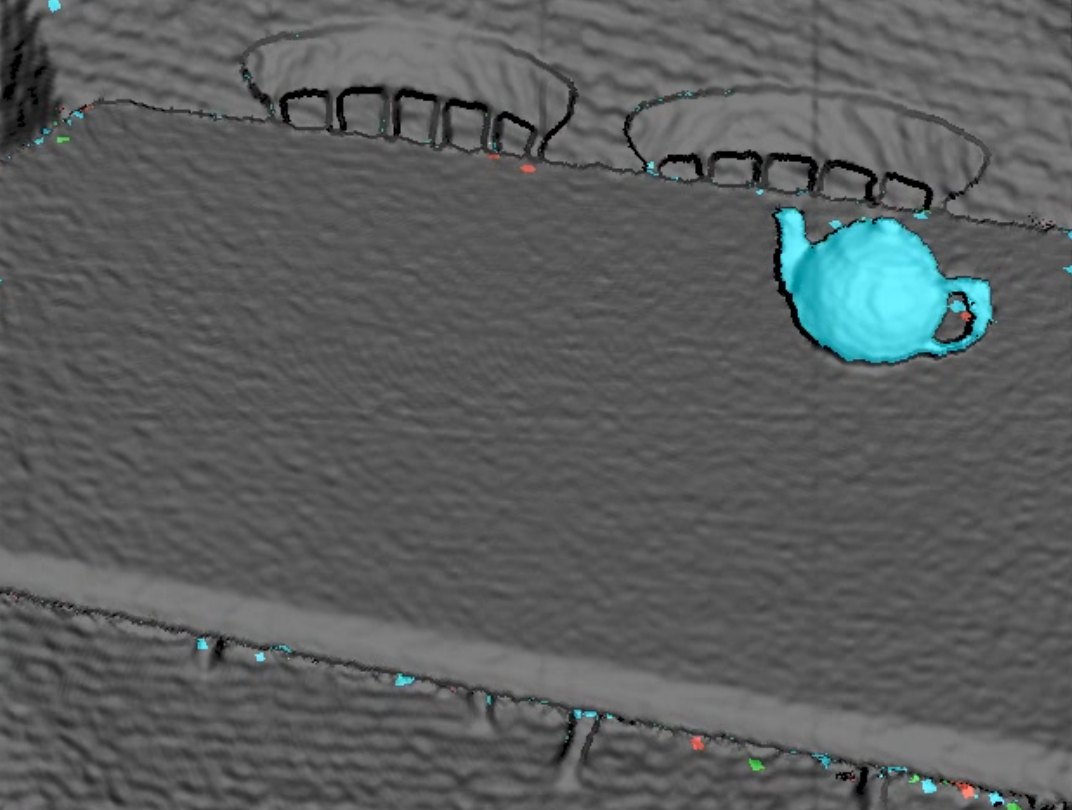
\includegraphics[width=.28\linewidth]{figures/moseg/objects2.png} &
    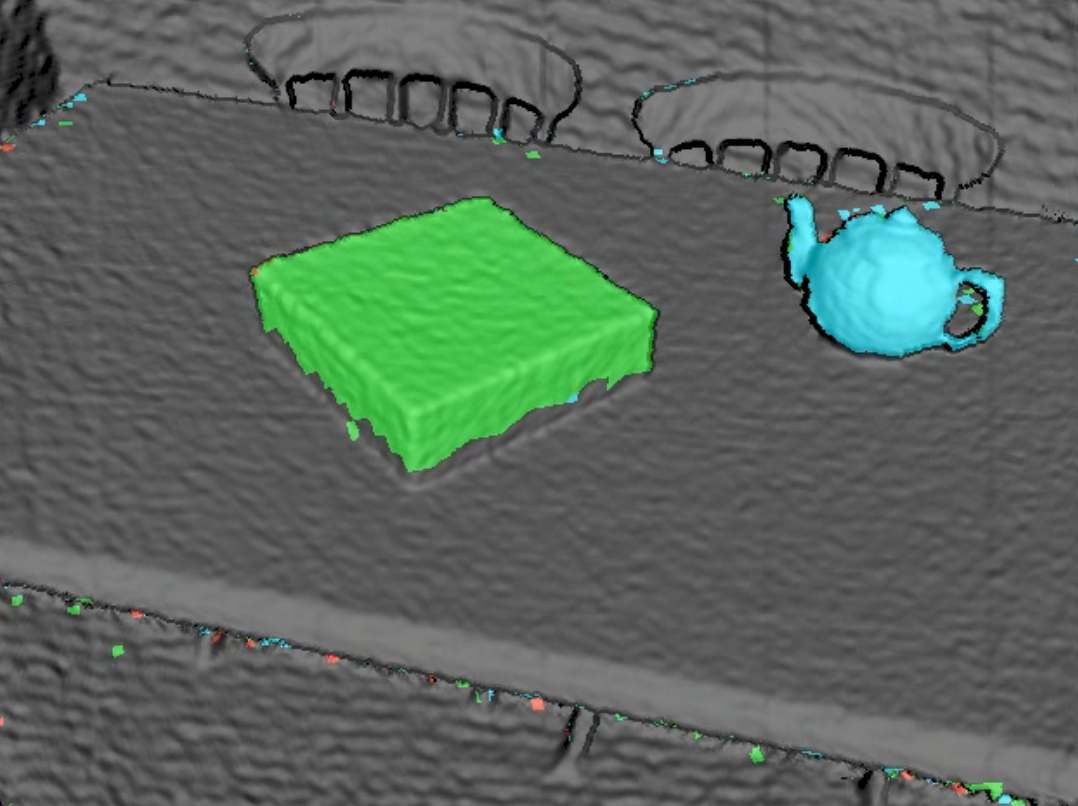
\includegraphics[width=.28\linewidth]{figures/moseg/objects3.png} \\ 
    (a) & (b) & (c) \\
    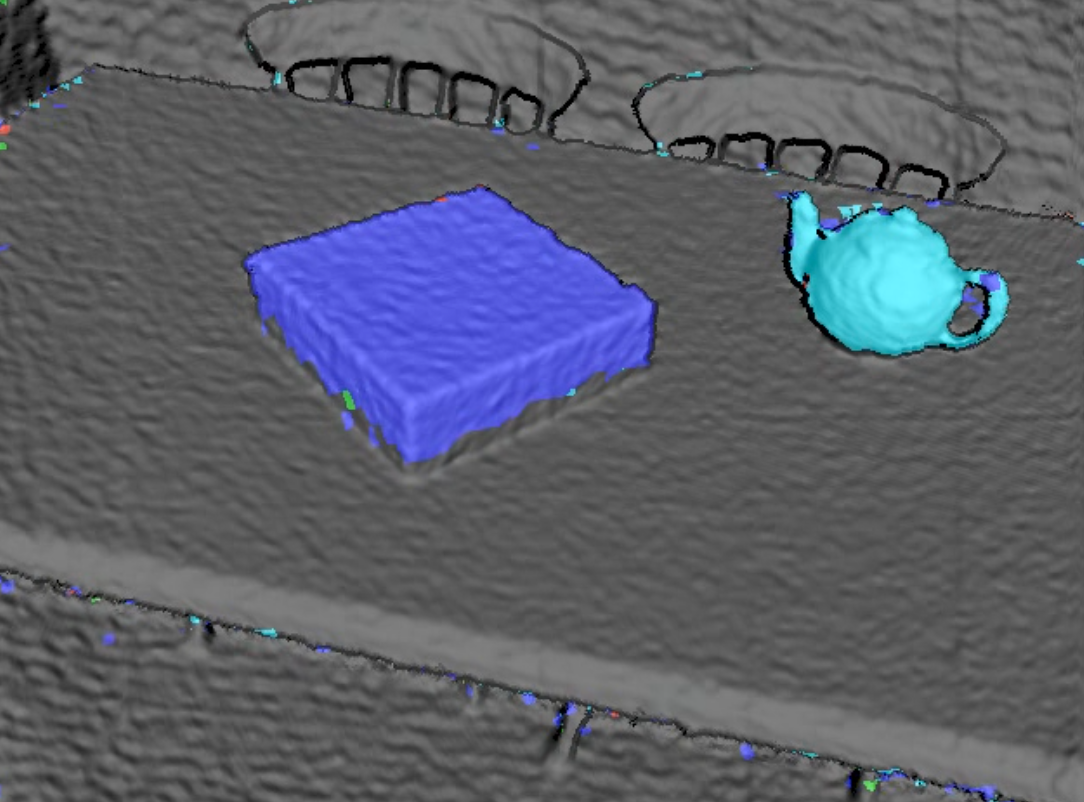
\includegraphics[width=.28\linewidth]{figures/moseg/objects4.png} &
    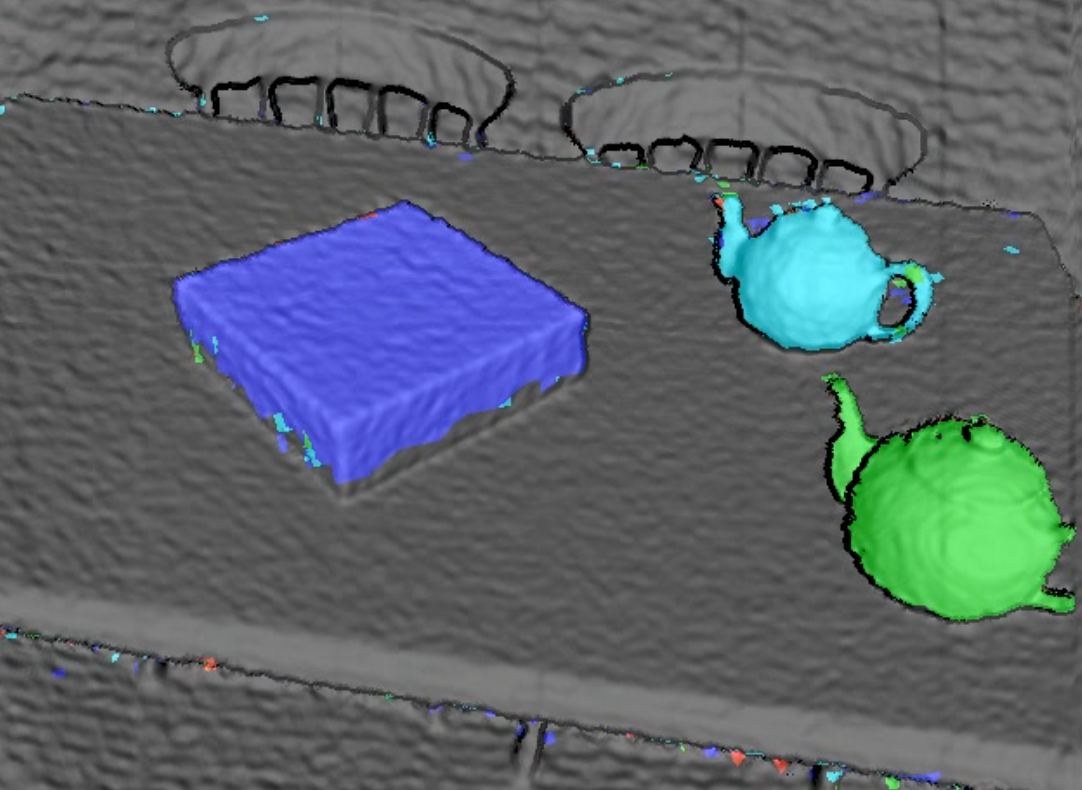
\includegraphics[width=.28\linewidth]{figures/moseg/objects5.png} &
    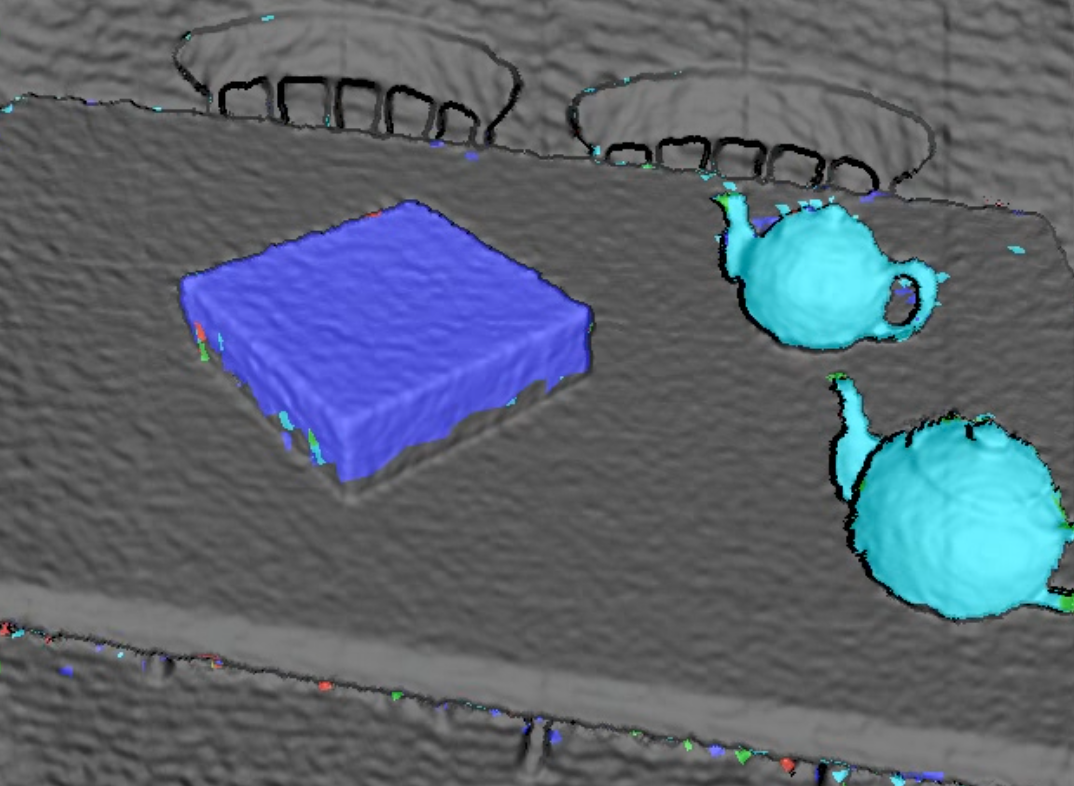
\includegraphics[width=.28\linewidth]{figures/moseg/objects6.png} \\ 
    (d) & (e) & (f) \\
  \end{tabular}
  \caption[Motion Segmentation Object Recognition]
  {An example of the training and prediction process for dynamic
    objects:
    (a) A teapot is placed in the scene;
    (b) The teapot is recognised as a new object and an SVM is trained for it;
    (c) A box is placed in the scene; (d) the box is recognised as being
    distinct from the teapot, and a separate SVM is trained for it;
    (e) Another teapot is placed in the scene; (f) the new teapot is recognised
    as being a teapot rather than a box, and is labelled accordingly.}
~\label{figure:moseg_recognition}
\end{figure}

\section{Summary}
~\label{sec:moseg_discussion}
As outlined in Sections~\ref{sec:moseg_qualitative} and~\ref{sec:moseg_quantitative}, the 
proposed approach provides an improvement on the quality of camera pose estimation when 
performing dense reconstruction in scenes that have dynamic components, versus the 
standard \textit{KinectFusion}~\cite{Newcombe2011} like pipeline as implemented by 
\textit{Prisacariu et al}~\cite{Prisacariu2014}; a research objective that was outlined in 
Section~\ref{sec:intro_aims_structure}.

Additionally, it is evident that the proposed approach is capable of segmenting dynamic 
components (such as people moving in an articulated fashion) that are visible in the camera's 
view frustrum, from those that are static (such as furniture in the scene). This segmentation 
also demonstrates a novel way of obtaining 3D geometry information to perform rudimentary scene 
understanding. Additionally, the resultant reconstructions of the proposed approach are 
qualitatively comparable to the comparison static dense SLAM system. Both of these results 
relate again to the research objectives of Section~\ref{sec:intro_aims_structure}.

The novel dual volumetric representation approach taken in this work of maintaining both a 
\textit{static} and a \textit{dynamic} scene, utilising only the former for camera pose 
estimation provides a simple and robust system for dense 3D reconstruction in environments 
that would otherwise be troublesome. Contrary to existing approaches outlined in Section 
~\ref{sec:lit_review_dynamic}, the presented system has scope for use in large-scale 
reconstruction scenarios, due to it's leverage of efficient, hashed volumetric data structures. 
In addition, by utilising such data structures, the proposed system is performant to the 
level of highly optimised~\cite{Prisacariu2014} \textit{KinectFusion}~\cite{Newcombe2011} 
implementations, demonstrating feasibility for application to problems that require 
real time performance.

With the contributions outlined in this work, the proposed approach provides a platform 
for further research into problems such as live semantic scene understanding and dense scene 
flow. The proposed approach has the potential to be further developed in to a fully dynamic, 
semantic scene understanding and reconstruction system for use in robotics, VR and AR applications 
as outlined in Section~\ref{sec:intro_scene_recon}.

\chapter{Probabilistic Object Reconstruction with Online Drift Correction}
\section{Introduction}
\label{sec:probobj_introduction}
Dense SLAM has proven to be an effective paradigm for the reconstruction of 
scenes of moderate size, with much research on the topic driven by the 
availability of consumer grade depth sensing equipment. However, there is a 
heavy reliance on descriptive geometry in the scene when there is a lack of 
texture. Less descriptive geometry leads to an increase in camera tracking 
error and causes model inconsistencies, especially when a loop closure event 
occurs. This is due to the small but cumulative errors incurred in pose 
estimation that prevent a reconstructed model from being closed when the 
camera return to it's staring position.

As object reconstruction can be seen as a smaller scale equivalent of the scene
based dense reconstruction problem, it too is prone to the tracking drift and
loop closure problems, sometimes to a prohibitive level. Often it may be
desirable to perform object reconstruction in an interactive way, for example,
as a component of a scene understanding system, or to procure training data for
the object in question.

With a high level of interaction comes an exacerbation of the aforementioned
shortcomings of dense SLAM, particularly due to the potential for frequent,
repetitive motion. This is the problem that is addressed in this chapter.

In this chapter, a probabilistic object reconstruction framework is presented
for the reconstruction of rigid objects based on object appearances.
The framework facilitates the correction of camera tracking drift by
representing the object to be reconstructed as a collection of overlapping
subsegments, such that deformations may be inferred to keep the subsegments
aligned, resulting in a consistent overall model. The system utilises a
volumetric representation for each of these object subsegments, as with many
larger scale reconstruction systems. Each voxel in the subsegments has
additional appearance posterior information pertaining to the voxels membership
of the object.

Over time, multiple volumes containing both surface and probabilistic appearance
information are maintained and manipulated to yield a robust and temporally
consistent model. Finally, the optimum object shape is optimised for within a 
Conditional Random Field (CRF) \cite{BishopPRML} framework.

The proposed system is inspired by that of \textit{Kolev et al} \cite{Kolev2006} 
in that the representation used for the shape of the object to be modelled is a 
volume of probabilities, pertaining to posteriors over a voxels assignment to 
being either on the objects surface or not. In the proposed system this volume 
of posterior probabilities is ``fused'' into with each frame, much like the 
fusion process in systems such as KinectFusion \cite{Newcombe2011} and 
InfiniTAM \cite{Prisacariu2014}.

The probabilities that are ``fused'' into the volume are generated from an
appearance model, initialised prior to reconstruction by a Maximum Likelihood 
Estimation (MLE) \cite{BishopPRML} procedure over the first frame of the RGB image. 
There are two appearance models, one for the foreground object and one for the 
background, with the foreground object indicated by a user inputted bounding box 
on the first RGB frame. An appearance distribution is fitted over the colour features 
of each class, foreground and background. During the fusion process, the PDF's of 
these distributions are evaluated on the latest colour observation for a voxel and 
posteriors are computed \& updated accordingly in the probability volume. Only 
those voxels with a posterior higher for the foreground than the background 
are rendered.

\section{Related Work}
\label{sec:probobj_related_work}

\section{Algorithm Overview}
In the proposed system, the object model is divided into \textit{subvolumes}, 
each consisting of a TSDF, colour volume and object Probability Volume. 
Additionally, each has associated with it a rigid body transform 
$\mathbf{T} \in \mathbb{SE}(3)$ that specifies it's pose relative to the global 
coordinate frame.

At each time step, a segmentation model is applied to the RGB input image to
generate an object \textit{Probability Map} defining the segmented region to be
the object of interest and the remainder the background, to be discarded. Using
these generated Probability Maps, the system accumulates the probabilities into
the object \textit{Probability Volume} of the active subvolume.

As with the dense SLAM system outlined earlier in this work, the proposed system
also has \textit{Integration}, \textit{Tracking} and \textit{Rendering}
stages in it's pipeline (all of which are run at each time step). However, in
the proposed system, there are an additional two stages to the pipeline;
\textit{Online Model Correction} and \textit{CRF Based Segmentation}.

At the end of each frame, the online model correction algorithm is run, which
infers the relative poses between the subvolumes, mitigating tracking drift.
Once the reconstruction process is finished, a CRF-based optimisation is 
performed to refine the resulting object segmentation over all subvolumes.

The proposed approach is not tied to the use of any one probabilistic model,
though in the presented experiments Pixel Wise Posteriors (PwP) of \textit{Bibby et al} 
\cite{Bibby2008} are used. An overview of the object reconstruction pipeline is shown in
Figure \ref{fig:probobj_pipeline_diagram}.

\begin{figure}[h]
  \label{fig:probobj_pipeline_diagram}
  \centering
  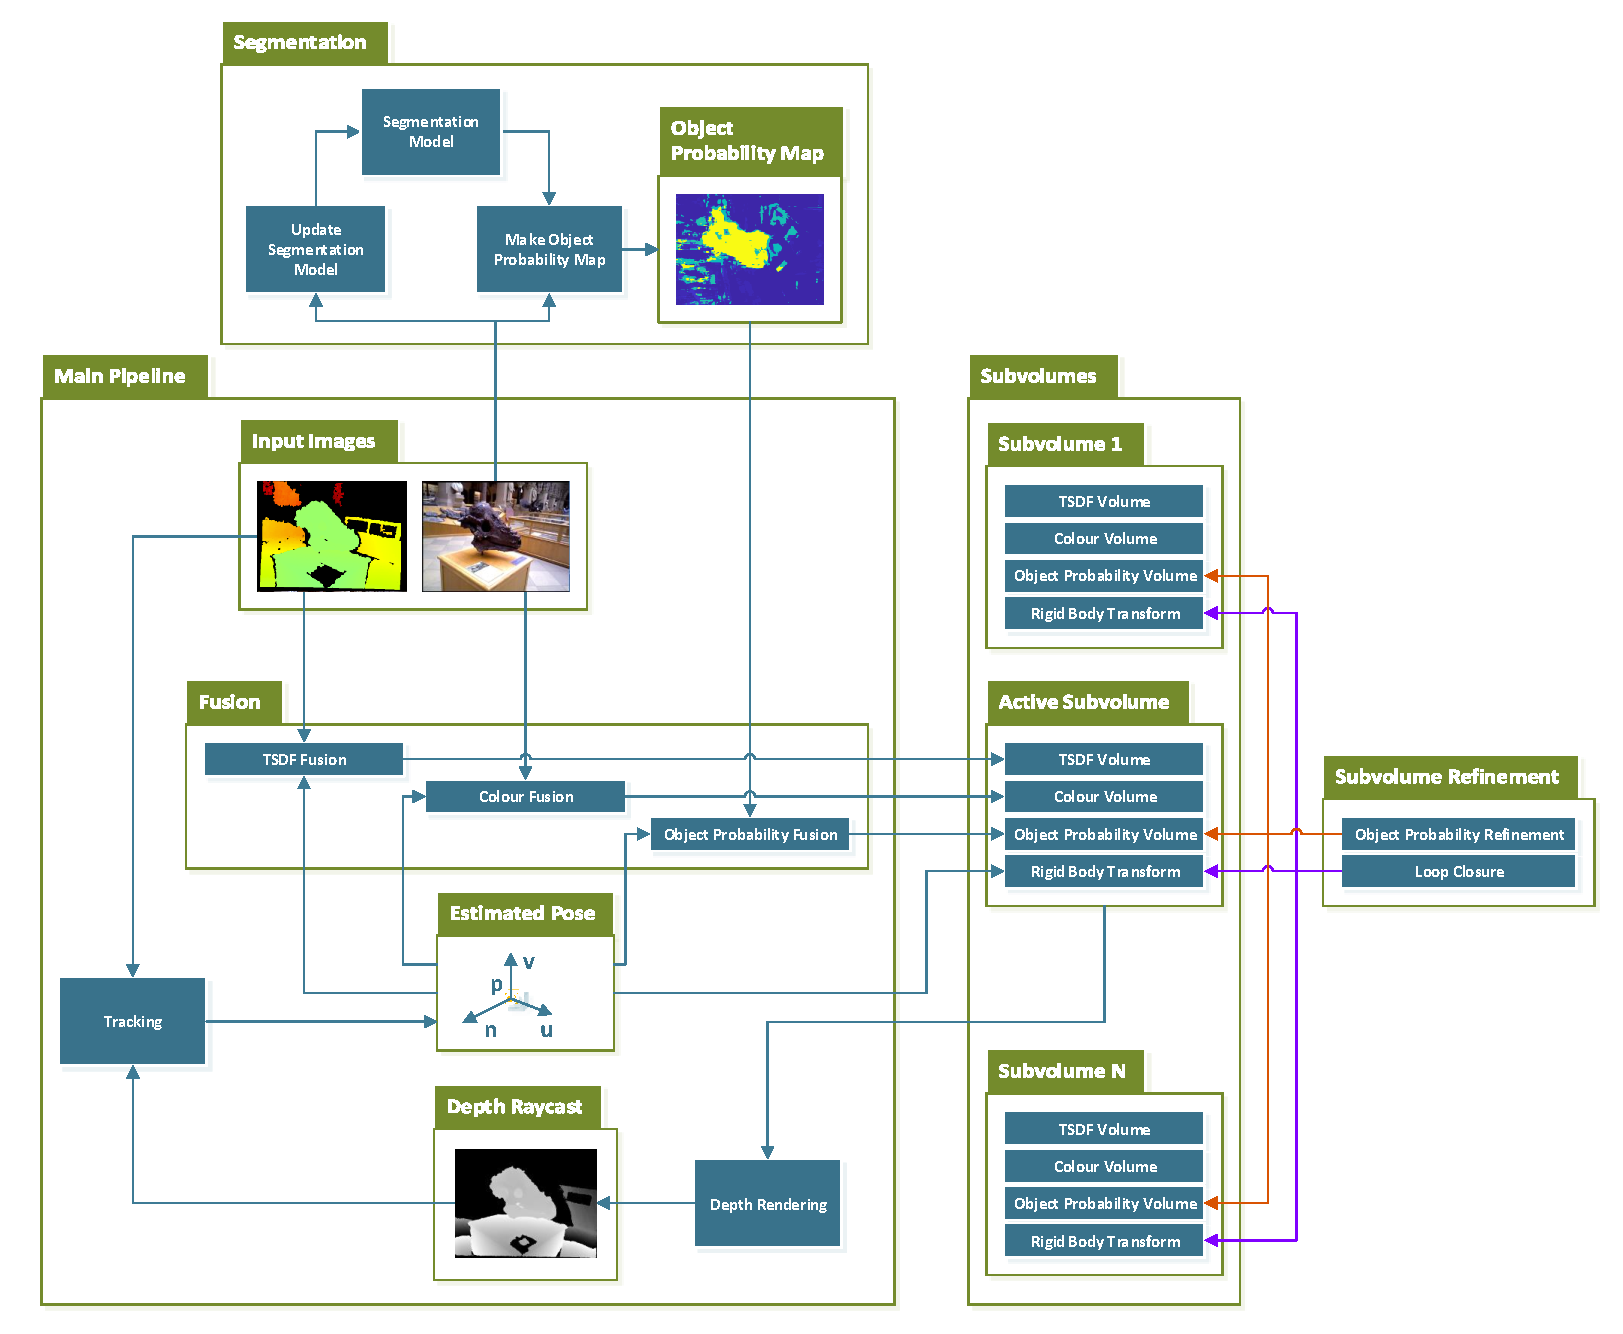
\includegraphics[width=\linewidth]{figures/object_recon/pipeline.pdf}
  \caption[Probabilistic Object Reconstruction Pipeline]
  {The pipeline of the proposed Object Reconstruction approach.}
\end{figure}

\section{Probabilistic Formulation of Object Reconstruction}
\label{sec:probobj_prob_formulation}
The surface map and camera pose are estimated using the standard KinectFusion
like pipeline of \cite{Newcombe2011,Prisacariu2014}. The surface is represented
as the Zero Level Set of a TSDF discretised over voxels, with the isosurface 
embedding built by a weigted mean of new observations, as outlined in Equations
\ref{eqn:sdf_update} and \ref{eqn:sdf_weight_update}. Camera pose estimation is
performed with ICP, as outlined in Section \ref{subsec:moseg_static_camera_trackin} 
and is run quasi-simultaneously against the evolving map. Here, inspired by 
\cite{Kolev2006}, this procedure is augmented by estimating the posterior probability, 
per map voxel, of belonging to the object of interest. This volume of posterior 
probabilities is updated at each time step, in parallel to the fusion process in the 
mapping and pose estimation components of the pipeline. The representation of the 
reconstructed object comprises multiple ``subvolumes'', each pertaining to some 
patch on the object surface. New subvolumes are created when sufficiently many new 
voxels have been allocated and have had SDF data integrated. By ensuring overlap
between the subvolumes, transformations between them can be found and pose
inconsistencies addressed, online. Empirically, the threshold for starting a new
subvolume is defined as the event when $50\%$ of the voxels fused in to the
current volume are newly observed points, such that there is sufficient overlap 
between two subvolumes that shall later be registered.

\subsection{Volumetric Appearance Model}
\label{subsec:probobj_vol_appearance_model}
At each observed RGBD frame, the object posterior probabilities for the visible
voxels in the active subvolume are updated via an appearance-derived probability
map for that frame. Under the assumption of conditional independence between
frames (for sake of tractability), the posterior probability of a given voxel
$\psi \in \Psi$ belonging to the object has the following form(noting that
$\Phi \subset \Psi$):
\begin{equation}
\label{eqn:probobj_voxel_posterior}
P(\psi \in \Phi | \Omega, p) = \prod_{t=0}^{\infty}
P(\psi_{t} \in \Phi | \Omega_{t}, p_{t})
\end{equation}
where $\Psi$ is the volume of voxels for which measurements are accumulated,
$\Phi$  is the volume of voxels pertaining to the object $\mathbf{\Phi}$ of 
interest, $\Omega_{t}$ is the current RGBD image observation at time $t$ and 
$p_{t}$ is the currently tracked pose at time $t$. Equation 
\ref{eqn:probobj_voxel_posterior} encodes the probability of a voxel belonging 
to the object of interest as the product of instantaneous appearance-derived 
pixel-wise conditionals. Note that in the above, $\Phi$ is a discretisation of 
the continuous $\Phi$ in the probabilistic formulation that follows.

\subsection{Full Joint Definition}
\label{subsec:probobj_full_joint}
Central to the proposed system is the aforementioned volume of appearance based
posterior probabilities pertaining to a voxel wise membership of either the
object voxel set or the non object (background) voxel set. This allows
formulation of the full joint distribution over the object as the Probabilistic
Graphical Model (PGM) of Figure \ref{fig:probobj_pgm1}.
\begin{figure}[h]
  \label{fig:probobj_pgm1}
  \centering
  \resizebox {0.4\linewidth}{!}{
    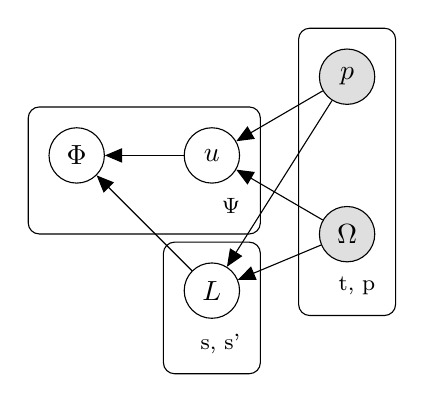
\begin{tikzpicture}
      % Declare nodes.
      \node[latent] (phi) {$\Phi$};
      \node[latent, right=of phi] (u) {$u$};
      \node[latent, below=of u] (L) {$L$};
      \node[obs, right=of u, yshift=-1cm] (omega) {$\Omega$};
      \node[obs, right=of u, yshift=1cm] (p) {$p$};
      
      % Setup plates.
      \plate[inner sep=0.25cm] {plate1} {(omega) (p)} {t, p};
      \plate[inner sep=0.25cm] {plate2} {(u) (phi)} {$\Psi$};
      \plate[inner sep=0.25cm] {plate3} {(L)} {s, s'};
      
      % Setup edges.
      \edge {omega, p} {u, L}
      \edge {L} {phi}
      \edge {u} {phi}
    \end{tikzpicture}
  }
  \caption[Probabilistic Object Reconstruction Formulation I]
  {Probabilistic Graphical Model representing the full Joint
    Distribution over the shape $\mathbf{\Phi}$ of the object of interest.}
\end{figure}

Where $\Phi$ is the shape of the object to be reconstructed (represented as a
subset of voxels for which surface data has been integrated into the relevant
TSDF), $u$ is the appearance model volume (aforementioned appearance Posteriors 
of Equation \ref{eqn:probobj_voxel_posterior}), $L$ is the set of consistency 
constraints for each adjacent sub volume pair in the form of rigid body 
transformations, $\Omega$ is the set of RGBD image pixels and $p$ the set of 
poses over time.

The PGM given in Figure \ref{fig:probobj_pgm1} leads to the following
factorisation over the full Joint Distribution.
\begin{equation}
  \label{eqn:probobj_full_joint}
  P(\Phi, \Omega, p, u, L) = 
  \prod_{\psi \in \Psi}\prod_{s, s' \in \mathcal{S}}
  P(\Phi \given u_{\psi}, L_{s, s'}) 
  \prod_{t=0}^{\infty}\prod_{p \in \mathcal{P}}
  P(u_{\psi} \given \Omega_{p, t}, p_{t})
  P(L_{s, s'} \given \Omega_{p, t}, p_{t})
  P(L_{s, s'})P(p_{t})P(\Omega_{p, t})
\end{equation}
Where in Equation \ref{eqn:probobj_full_joint}, $\Psi$ is the set of voxels
across all subvolumes, $\mathcal{P}$ is the set of RGBD pixels for a given 
frame $\Omega_{t}$ and $\mathcal{S}$ is the set of subvolumes. Note that the 
notation $s, s' \in \mathcal{S}$ refers to pairs of adjacent, overlapping 
subvolumes.

If pixel-wise independence is assumed in the RGBD observations and temporal
independence is assumed in the poses, the plate containing $\Omega$ and $p$ can
be removed as shown in Figure \ref{fig:probobj_pgm2}.
\begin{figure}[h]
  \label{fig:probobj_pgm2}
  \centering
  \resizebox {0.4\linewidth}{!}{
    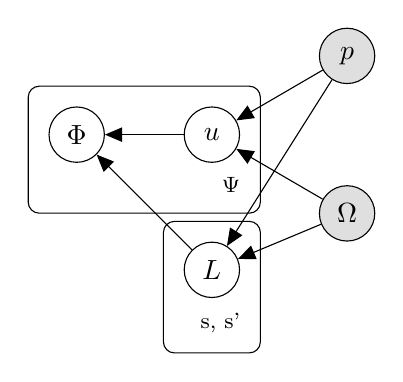
\begin{tikzpicture}
      % Declare nodes.
      \node[latent] (phi) {$\Phi$};
      \node[latent, right=of phi] (u) {$u$};
      \node[latent, below=of u] (L) {$L$};
      \node[obs, right=of u, yshift=-1cm] (omega) {$\Omega$};
      \node[obs, right=of u, yshift=1cm] (p) {$p$};
      
      % Setup plates.
      \plate[inner sep=0.25cm] {plate3} {(L)} {s, s'};
      \plate[inner sep=0.25cm] {plate2} {(u) (phi)} {$\Psi$};
      
      % Setup edges.
      \edge {omega, p} {u, L}
      \edge {L} {phi}
      \edge {u} {phi}
    \end{tikzpicture}
  }
  \caption[Probabilistic Object Reconstruction Formulation II]
  {Probabilistic Graphical Model representing the simplified Joint
    Distribution over the shape $\mathbf{\Phi}$ of the object of interest.}
\end{figure}

The simplifications transforming the PGM of Figure \ref{fig:probobj_pgm1} in to
that of Figure \ref{fig:probobj_pgm2} lead to the following factorisation of the
Joint Distribution over $\mathbf{\Phi}$.
\begin{equation}
  \label{eqn:probobj_simplified_joint}
  P(\Phi, \Omega, p, u, L) = 
  \prod_{\psi \in \mathbf{\Psi}}P(\Phi \given u_{\psi})
  \prod_{s, s' \in \mathcal{S}}P(u_{\psi} \given \Omega, p, L_{s, s'})
  P(L_{s, s'} \given \Omega, p) P(L_{s, s'})P(p)P(\Omega)
\end{equation}

The formalisms defined in Figures \ref{fig:probobj_pgm1} and
\ref{fig:probobj_pgm2} and Equations \ref{eqn:probobj_full_joint} and
\ref{eqn:probobj_simplified_joint} describe a probabilistic framework in which
online corrections can be made to the reconstructed model (piecewise over
subvolumes) to counter errors caused by pose tracking inconsistencies. As with
scene scale dense SLAM systems \cite{Newcombe2011, Prisacariu2014, NieBner2013},
the presented system follows a pipeline that consists of a tracking stage and an
integration stage, as outlined in Section \ref{sec:moseg_static_fusion}.

However, the presented formulation of this pipeline consists of an
additional, novel estimation module that relies on the use of a subvolume
representation to correct tracking errors by applying rigid body transformations
to the subsegments of the reconstructed shape (the subvolumes) to correct their
alignment when there are intra subsegment tracking inconsistencies. As inference
on the Joint Distribution of the presented probabilistic model is intractable, 
conditional independence assumptions are made that empirically do not appear to 
cause any functional issues. 

Note that only voxels whose appearance posterior is greater for the foreground 
class are used in the correction procedure; only voxels that satisfy the probabilistic 
condition $P(\psi \in \Phi | \Omega, p) > 1 - P(\psi \in \Phi | \Omega, p)$ are 
considered.

\subsection{Appearance Marginal}
Continuing on from the formulation given in Equation \ref{eqn:probobj_simplified_joint}, 
the appearance model $u$ may be marginalised as follows.
\begin{align}
  \label{eqn:probobj_appearance_marginal}
  % Line 1.
  P(\Phi, \Omega, p, L) & =
  \int_{-\infty}^{\infty} \Bigg[ 
  \prod_{\psi \in \mathbf{\Psi}} P(\Phi \given u_{\psi})
  \prod_{s, s' \in \mathcal{S}}P(u_{\psi} \given \Omega, p, L_{s, s'})
  P(L_{s, s'} \given \Omega, p) P(L_{s, s'})P(p)P(\Omega) \Bigg] \intd{u} \\
  % Line 2.
  & = \prod_{\psi \in \mathbf{\Psi}} 
  \int_{-\infty}^{\infty} \Bigg[ P(\Phi \given u_{\psi})
  \prod_{s, s' \in \mathcal{S}}P(u_{\psi} \given \Omega, p, L_{s, s'})
  P(L_{s, s'} \given \Omega, p) P(L_{s, s'})P(p)P(\Omega) \Bigg] \intd{u} \\
  & = \prod_{s, s' \in \mathcal{S}} P(L_{s, s'} \given \Omega, p)
  P(L_{s, s'})P(p)P(\Omega)P(\mathbf{\Phi})
\end{align}
Note that the Appearance Posterior Volume outlined in Section 
\ref{subsec:probobj_vol_appearance_model} is reintroduced later in this work in
Section \ref{} for the purposes of subvolume alignment and determining the
subset of voxels $\mathbf{\Phi} \subset \mathbf{\Psi}$ that determine the target
object shape.

Further details pertaining to the inference procedure for the per-subvolume
deformations is provided in Section \ref{sec:probobj_model_correction}.

\section{Online Model Correction}
\label{sec:probobj_model_correction}
The tracking consistency constraints denoted by the variables $L_{s, s'}$ such
that $s, s' \in \mathcal{S}$ with $\mathcal{S}$ being the set of overlapping
subvolume pairs $s, s'$ in the Probabilistic Graphical Models given by Figures
\ref{fig:probobj_pgm1} and \ref{fig:probobj_pgm2} can be enforced in terms of
minimising the disparity between each pair of adjacent subvolumes. The effect of
this minimsation being that consistency in the pose estimation phase of the
pipeline outlined in Figure \ref{fig:probobj_pipeline_diagram} is enforced. The
objective of this procedure is to infer a robust and consistent deformation
transformation for the subvolume pair.

\subsection{Alignment MAP Estimate}
\label{subsec:probobj_alignment_map}
Referring back to the joint distribution of Equation \ref{eqn:probobj_simplified_joint}, 
to achieve the aforementioned minimisation of disparity between overlapping subvolumes, 
a Maximum a Posteriori (MAP) estimate is desirable. As such, a MAP estimate over $L_{s, s'}$ 
in Equation \ref{eqn:probobj_simplified_joint} for a given subvolume pair $s, s'$ may be
derived as follows.
\begin{align}
  \label{eqn:probobj_map_estimate}
  % Line 1.
  P(\Omega, p | L_{s, s'}) & \propto \prod_{s, s' \in \mathcal{S}}
  \frac{P(L_{s, s'} | \Omega, p) 
  P(\Omega | p)P(p)P(L_{s, s'})}
  {\displaystyle\int_{-\infty}^{\infty} P(L_{s, s'} \given \Omega, p)
  \intd{L_{s, s'}}} P(\Phi) \\
  % Line 2.
  & \propto \prod_{s, s' \in \mathcal{S}} P(L_{s, s'} | \Omega, p) P(\Omega | p)
  P(p)P(L_{s, s'})P(\Phi) \\
  % Line 3.
  & \propto \prod_{s, s' \in \mathcal{S}} P(L_{s, s'} | \Omega, p)P(L_{s, s'})
  P(\Phi)
\end{align}
Note that in the third step of Equation \ref{eqn:probobj_map_estimate} the
distributions $P(\Omega | p)$ and $P(p)$ are taken to be uniform and as such may
be omitted whilst retaining proportionality. The prior distribution $P(L_{s, s'})$ is
conjugate to $P(L_{s, s'} | \Omega, p)$ and is of the form of a Multivariate
Gaussian Distribution $\mathcal{N}(\mathbf{0} \given \mathbf{I})$ over the
$\mathbb{SE}(3)$ deformation parameters described in Section 
\ref{subsub:moseg_static_camera_attitude}. The choice of such a prior distribution
is motivated by the assumption that motion between consecutive frames is minor,
thus the given prior will have the effect of constraining the $\mathbb{SE}(3)$
transformation as such. The prior distribution $P(\Phi)$ serves as a
\textit{Surface Prior} to mitigate the effect of noise introduced in to the TSDF
volumes. The form of $P(\Phi)$ shall be discussed in Section
\ref{subsec:probobj_analytic_alignment_map}.

The rationale of Equation \ref{eqn:probobj_map_estimate} is that the deformation
$L_{s, s'}$ applied to the subvolume $s$ maximises the posterior probability of
observing the current pose $p$ given the current RGBD frame $\Omega$ by reducing
the variance of the result of the pose estimation phase of the pipeline. As such,
global tracking variance (quantified by the proportion of outliers in the result
of the ICP component of the pipeline) is reduced by enforcing local consistency,
also improving global consistency and thus the quality of the resultant
reconstruction.

\subsection{Analytic Form of Alignment MAP Estimate}
\label{subsec:probobj_analytic_alignment_map}
With the probabilistic framework now outlined, the analytic form of the
posterior given in Equation \ref{eqn:probobj_map_estimate} may be explored. The
likelihood term in Equation \ref{eqn:probobj_map_estimate} quantifies the
ability of the constraint $L_{s, s'}$ to maximise consistency between subvolumes
$s$ and $s'$, with respect to observed RGBD frame $\Omega$ and pose $p$. By
quantifying the likelihood only for voxels in $s$ and $s'$ that are visible in
the current view frustrum at time $t$, the posterior $P(\Omega, p | L_{s, s'})$
is given. As outlined in Section \ref{subsec:probobj_alignment_map}, the prior
on the constraints $L_{s, s'}$ has the form of a Multivariate Gaussian
Distribution of the form $\mathcal{N}(\mathbf{0}, \mathbf{I})$.

As such, the analytic form of the likelihood term $P(L_{s, s'} | \Omega, p)$ is
given as follows.
\begin{equation}
  \label{eqn:probobj_likelihood_analytic}
  P(L_{s, s'} | \Omega, p) = \prod_{(s, s') \in \mathcal{S}}
  \frac{1}{\sqrt{2 \pi \sigma}}
  \exp{\frac{-\Big[\Phi_{s}\Big(\mathbf{x}\Big) -
  \Phi_{s'}\Big(\Lambda(\mathbf{x}, \mathbf{p}, \mathbf{t})\Big)\Big]^{2}}
  {2\sigma^{2}}}
\end{equation}

In Equation \ref{eqn:probobj_likelihood_analytic}, the function $\Lambda(.)$
applies the resultant $\mathbb{SE}(3)$ transform to a given voxel position
$\mathbf{x}$ and is defined as follows.
\begin{align}
  \label{eqn:probobj_lambda_fn}
  \Lambda(\mathbf{x}, \mathbf{p}, \mathbf{t}) &=
  \mathbf{R}_{\mathbf{p}} \mathbf{x} + \mathbf{t}\\
  &= 
  \begin{bmatrix}
    \mathbf{R}_{\mathbf{p}} & \mathbf{t} \\
    \mathbf{0} & 1
  \end{bmatrix}
  \mathbf{x}
\end{align}
In Equation \ref{eqn:probobj_lambda_fn} $R_{\mathbf{p}}$ is the $\mathbb{SO}(3)$
rotation matrix generated from the Rodrigues parameters given by the Vector
$\mathbf{p}$. Recall the definition of the Rodrigues paramaterisation given in
Equation \ref{eqn:rodriguez_matrix_eq} of Section
\ref{subsub:moseg_static_camera_attitude}.

The form of the aforementioned surface prior $P(\Phi)$ is taken to be that of
the Logistic Distribution, due to the ``symmetric'' $1 - f(x) = f(-x)$
and ``squashing'' $\texttt{Range}[f(x)] = [0, 1]$ properties of it's Cumulative
Density Function (CDF). The PDF of the Logistic Distribution is given as follows.
\begin{equation}
  \label{eqn:probobj_logistic_dist}
  \text{Logistic}(x \given \mu, \sigma) = \frac
  {e^{-\frac{x - \mu}{\sigma}}}
  {\sigma \big( 1 + e^{-\frac{x - \mu}{\sigma}} \big)^{2}}
\end{equation}

To encode the probability of a given voxel $\psi \in \mathbf{\Psi}$ encoding an
isosurface point, represented as the Zero Level Set defined in Equation
\ref{eqn:zero_level_definition} of a TSDF, it is desirable to quantify the
probability with a function that has the aforementioned properties. As such, the
CDF of $P(\Phi)$ is derived as follows.
\begin{align}
  \label{eqn:probobj_surface_prior_cdf}
  % Line 1.
  %P(\Phi < b) &= \int_{-\infty}^{b} \text{Logistic}
  %(\Phi \given \mu, \sigma) \intd{\Phi}\\
  % Line 2.
  \bar{P}(\Phi) &\propto P(\Phi < b)\\
  &\propto \int_{-\infty}^{b} \frac
  {e^{-\frac{\Phi - \mu}{\sigma}}}
  {\sigma \Big( 1 + e^{-\frac{\Phi - \mu}{\sigma}} \Big)^{2}} \intd{\Phi}\\
  % Line 3.
  &\propto \lim_{y\to -\infty} \int_{y}^{b} \frac
  {e^{\frac{-\Phi + \mu}{\sigma}}}
  {\sigma \Big( 1 + e^{\frac{-\Phi + \mu}{\sigma}} \Big)^{2}} \intd{\Phi}\\
  % Line 4.
  &\propto \lim_{y\to -\infty} \frac{1}{\sigma} \int_{y}^{b}
  \frac{e^{\frac{u}{s}}}{\Big( 1 + e^{\frac{u}{\sigma}} \Big)^{2}} \intd{u}\\
  \shortintertext{Where $u = -\Phi + \mu$ and $\intd{u} = -\intd{\Phi}$}
  % Line 5.
  &\propto \lim_{y\to -\infty} -\int_{y}^{b}
  \frac{e^{p}}{\Big( 1 + e^{p} \Big)^{2}} \intd{p}\\
  \shortintertext{Where $p = \frac{u}{\sigma}$ and $\intd{p} = \frac{1}{\sigma}
  \intd{u}$}
  % Line 6.
  &\propto \lim_{y\to -\infty} -\int_{y}^{b} \frac{1}{w^{2}} \intd{w}\\
  \shortintertext{Where $w = 1 + e^{p}$ and $\intd{w} = e^{p} \intd{p}$}
  % Line 7.
  &\propto \lim_{y\to -\infty} \Bigg[ \frac{1}{w} + C \Bigg]_{y}^{b}\\
  % Line 8.
  &\propto \lim_{y\to -\infty} \Bigg[ \frac{1}{1 + e^{p}} + C \Bigg]_{y}^{b}\\
  % Line 9.
  &= \lim_{y\to -\infty} \Bigg[ \frac{1}{1 +e^{\frac{u}{\sigma}}} + C
  \Bigg]_{y}^{b}\\
  % Line 10.
  &\propto \lim_{y\to -\infty} \Bigg[ \frac{1}{1 + e^{\frac{-\Phi + \mu}{\sigma}}} +
  C \Bigg]_{y}^{b}\\
  &\propto \Bigg[ \frac{1}{1 + e^{\frac{-\Phi + \mu}{\sigma}}} + C \Bigg]_{\Phi = b}
  - \Bigg[ \left. \lim_{y\to -\infty} \frac{1}{1 + e^{\frac{-\Phi + \mu}{\sigma}}}
  \right\rvert_{\Phi = y} + C \Bigg]\\
  &\propto \frac{1}{1 + e^{\frac{-\Phi + \mu}{\sigma}}}
\end{align}
Given the Cumulative Density Function derived in Equation
\ref{eqn:probobj_surface_prior_cdf}, the prior $P(\Phi)$ is defined as follows.
\begin{align}
  \label{eqn:probobj_surface_prior}
  \bar{P}(\Phi) &\propto \left. \int_{-\infty}^{b} \frac
  {e^{-\frac{\Phi - \mu}{\sigma}}}
  {\sigma \Big( 1 + e^{-\frac{\Phi - \mu}{\sigma}} \Big)^{2}} \intd{\Phi}
  \right\rvert_{\mu = 0, \sigma = 1}\\
  &\propto \frac{1}{1 + e^{-\Phi}}
\end{align}
It is evident from Equation \ref{eqn:probobj_surface_prior} that under an 
appropriate paramaterisation, the CDF of the Logistic Distribution is the 
Logistic Sigmoid function prevelant in the Artificial Neural Network literature. 
As given in Equation \ref{eqn:probobj_surface_prior} the mean $\mu$ and standard 
deviation $\sigma$ are $0$ and $1$, respectively.

Finally, the analytic form of the log-posterior is given as follows, optimising
for the Rodrigues parameters $p$ and translation vector $t$ of the constraint
$L_{s, s'}$ between subvolumes $s$ and $s'$.
\begin{align}
  \label{eqn:probobj_log_posterior}
  % Line 1.
  \ln P(\Omega, p | L_{s, s'}) &\propto \ln
  \prod_{s, s' \in \mathcal{s}} P(L_{s, s'} | \Omega, p)P(L_{s, s'})\bar{P}(\Phi)\\
  % Line 2.
  &\propto \sum_{s, s' \in \mathcal{S}} \ln P(L_{s, s'} | \Omega, p) +
  \sum_{s, s' \in \mathcal{S}} \ln P(L_{s, s'}) +
  \sum_{s, s' \in \mathcal{S}} \ln \bar{P}(\Phi)\\
  % Line 3.
  &\propto \sum_{s, s' \in \mathcal{S}} \Bigg[\ln \frac{1}{\sqrt{2 \pi \sigma}}
  \exp{\frac{-\Big[\Phi_{s}\big(\mathbf{x}\big) - \Phi_{s'}
  \big(\Lambda(\mathbf{x}, \mathbf{p}, \mathbf{t})\big)\Big]^{2}}
  {2\sigma^{2}}} \\
  &\phantom{\propto \sum_{s, s' \in \mathcal{S}} \Bigg[} % SPLIT LINE
  + \ln \frac{-\frac{1}{2} e^{\mathbf{p}^{T}\mathbf{\Sigma}^{-1}\mathbf{p}}}
  {\sqrt{(2\pi)^{k}\left|\mathbf{\Sigma}\right|}} +
  \ln \frac{1}{1 + e^{-\Phi}}\Bigg]\\
  % Line 4.
  &\propto \sum_{s, s' \in \mathcal{S}} \Bigg[ -\ln(2\pi\sigma) -
  \frac{\Big[\Phi_{s}\big(\mathbf{x}\big) -
  \Phi_{s'}\big(\Lambda(\mathbf{x}, \mathbf{p}, \mathbf{t})\big)\Big]^{2}}{2\sigma^{2}} -
  \frac{1}{2} \ln \left|\mathbf{\Sigma}\right|\\ 
  &\phantom{\propto \sum_{s, s' \in \mathcal{S}} \Bigg[} % SPLIT LINE
  - \frac{1}{2} \mathbf{p}^{T}\mathbf{\Sigma}^{-1}\mathbf{p} -
  \ln(1 + e^{-\Phi}) \Bigg]\\
  % Line 5.
  &\propto \sum_{s, s' \in \mathcal{S}} \Bigg[ -\ln(2\pi\sigma) -
  \frac{\Big[\Phi_{s}(\mathbf{x}) -
  \Phi_{s'}\big(\Lambda(\mathbf{x}, \mathbf{p}, \mathbf{t})\big)\Big]^{2}}{2\sigma^{2}} -
  \frac{1}{2} \mathbf{p}^{T}\mathbf{p} \\
  &\phantom{\propto \sum_{s, s' \in \mathcal{S}} \Bigg[} % SPLIT LINE
  - \ln(1 + e^{-\Phi}) \Bigg]
\end{align}

As with the gradients derived in Section \ref{subsec:moseg_static_camera_tracking}, the 
gradient update when optimising Equation \ref{eqn:probobj_log_posterior} takes the familiar 
Levenberg-Marquardt update form, akin to that of Equation \ref{eqn:lm_update}.

\subsection{Optimisation for MAP Inference}
\label{subsec:probobj_map_optimisation}
To infer the optimal consistency constraints between adjacent subvolumes, the
log-posterior given in Equation \ref{eqn:probobj_log_posterior} may be optimised
using second order gradient based methods such as Levenberg-Marquardt. As with
the ICP procedure outlined in Section \ref{subsub:moseg_static_camera_poserec},
the optimisation is performed with respect to the three Rodrigues rotation
parameters $\alpha$, $\beta$, $\gamma$ and translation parameters $t_{x}$,
$t_{y}$ and $t_{z}$ of the target $\mathbb{SE}(3)$ transformation.

In a similar manner to the process outlined in Section
\ref{subsub:moseg_static_camera_poserec}, the target energy function must be
differentiated with respect to each of the $\mathbb{SE}(3)$ parameters. In this
case, the log-posterior of Equation \ref{eqn:probobj_log_posterior} is the
target energy function and shall be denoted $E(.)$ in the following derivation.
The derivation of the partial derivatives of $E(.)$ with respect
to the Rodrigues rotational parameters is as follows for some parameter
$\tau \in \{\alpha, \beta, \gamma\}$.
\begin{align}
  \label{eqn:probobj_log_post_rot_grad}
  % Line 1.
  \frac{\partial E}{\partial \tau} &=
  \sum_{s, s' \in \mathcal{S}} \Bigg[ - \frac{\partial}{\partial \tau}
  \ln(2\pi\sigma) - \frac{\partial}{\partial \tau}
  \frac{\Big[\Phi_{s}\big(\mathbf{x}\big) -
  \Phi_{s'}\big(\Lambda(\mathbf{x})\big)\Big]^{2}}{2\sigma^{2}} -
  \frac{\partial}{\partial \tau} \frac{1}{2} \mathbf{p}^{T}\mathbf{p} -
  \frac{\partial}{\partial \tau} \ln(1 + e^{-\Phi})
  \Bigg]\\
  % Line 2.
  &= \sum_{s, s' \in \mathcal{S}} \Bigg[ \frac{1}{2\sigma^{2}}
  \frac{\partial}{\partial \tau}
  \Big[\Phi_{s}\big(\mathbf{x}\big) - \Phi_{s'}\big(\Lambda(\mathbf{x})\big)\Big]^{2} -
  \frac{1}{2} \frac{\partial}{\partial \tau}
  \mathbf{p}^{T}\mathbf{p} - \frac{\partial}{\partial \tau} \ln(1 + e^{-\Phi})
  \Bigg]\\
  % Line 3.
  &= \sum_{s, s' \in \mathcal{S}} \Bigg[ \frac{1}{2\sigma^{2}}
  \frac{\partial \phi}{\partial \Phi} \frac{\partial \Phi}{\partial \Lambda}
  \frac{\partial \Lambda}{\partial \mathbf{R}_{\tau}} -
  \frac{1}{2} \frac{\partial}{\partial \tau}
  \mathbf{p}^{T}\mathbf{p} - \frac{\partial}{\partial \tau} \ln(1 + e^{-\Phi})
  \Bigg]\\
  \shortintertext{Where $\phi(.) =
  \big(\Phi_{s}(\mathbf{x}) - \Phi_{s'}(\Lambda(\mathbf{x}))\big)^{2}$}
  % Line 4.
  &= \sum_{s, s' \in \mathcal{S}} \Bigg[ \sigma^{2} \phi(.)
  \frac{\partial \Phi}{\partial \Lambda}
  \frac{\partial \Lambda}{\partial \mathbf{R}_{\tau}} -
  \frac{1}{2} \frac{\partial}{\partial \tau}
  \mathbf{p}^{T}\mathbf{p} - \frac{\partial}{\partial \tau} \ln(1 + e^{-\Phi})
  \Bigg]\\
  % Line 5.
  &= \sum_{s, s' \in \mathcal{S}} \Bigg[ \sigma^{2} \phi(.)
  \frac{\partial \Phi}{\partial \Lambda}
  \frac{\partial \Lambda}{\partial \mathbf{R}_{\tau}} - \mathbf{p}^{T} -
  \frac{\partial}{\partial \tau} \ln(1 + e^{-\Phi})
    \Bigg]\\
  % Line 6.
  &= \sum_{s, s' \in \mathcal{S}} \Bigg[ \sigma^{2} \phi(.)
  \frac{\partial \Phi}{\partial \Lambda}
  \frac{\partial \Lambda}{\partial \mathbf{R}_{\tau}} - \mathbf{p}^{T} +
  \frac{1}{1 + e^{\Phi}} \frac{\partial \Phi}{\partial \Lambda}
  \frac{\partial \Lambda}{\partial \mathbf{R}_{\tau}} \Bigg]
\end{align}

\section{Volumetric Segmentation and Explicit Loop Closure Detection}
The final component of the proposed pipeline performs a segmentation in three
dimensional observed model space to perform refinements over the appearance
posteriors that separate the voxels pertaining to the object of interest from
those that have irrelevant measurements integrated, i.e. background measurements
that have not been used to perform pose estimation and as such have not been rendered.

This segmentation is formulated within a CRF framework, with each node in the
CRF graph representing a set of neighbouring voxels in space, where connections
are made between adjacent voxel neighbourhoods. This segmentation process is
posed as an energy minimisation problem to optimise for a cut in downsampled
voxel space between observations pertaining to the object of interest and those,
of irrelevant observations, such that a segmentation in 3D is obtained. The
central purpose of this segmentation is to refine the resultant output model of
the proposed object reconstruction system. The described CRF model is depicted
in Figure \ref{fig:probobj_crf}

\begin{figure}[h]
  \label{fig:probobj_crf}
  \centering
  \resizebox {0.5\linewidth}{!}{
    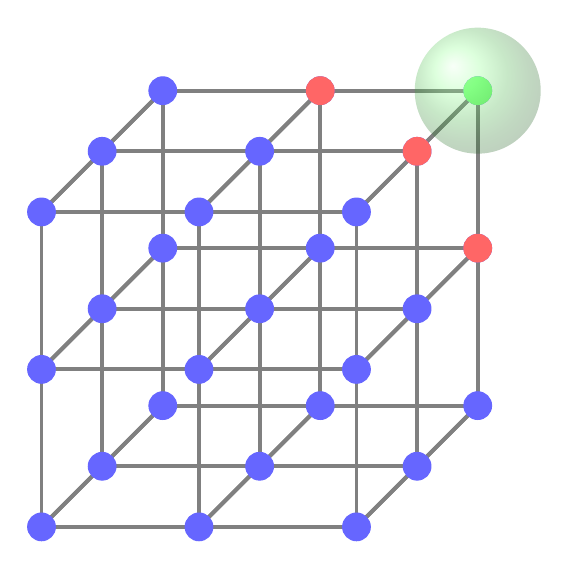
\begin{tikzpicture}[every node/.style={minimum size=1cm},on grid]
      % Define dimension and multiplier - tweakable.
      \newcommand\graphdim{2}
      \newcommand\multiplier{2}
      \newcommand\srad{0.8}

      % Define highlight node.
      \pgfmathtruncatemacro\hx{2}
      \pgfmathtruncatemacro\hy{2}
      \pgfmathtruncatemacro\hz{0}

      % Truncated Graph boundary nodes.
      \pgfmathtruncatemacro\gmin{-1}
      \pgfmathtruncatemacro\gmax{\multiplier*\graphdim + 1}

      % Draw Edges.
      \begin{scope}%[rotate around x=5]
        \foreach \i in {0,...,\graphdim}{
          \foreach \j in {0,...,\graphdim}{
            \foreach \k in {0,...,\graphdim}{
              % Get truncated x, y, and z. 
              \pgfmathtruncatemacro\x{\multiplier*\i}
              \pgfmathtruncatemacro\y{\multiplier*\j}
              \pgfmathtruncatemacro\z{\multiplier*\k}

              % Get truncated neigh left, right, up, down, forward and backward.
              \pgfmathtruncatemacro\nl{\x-\multiplier}
              \pgfmathtruncatemacro\nr{\x+\multiplier}
              \pgfmathtruncatemacro\nu{\y+\multiplier}
              \pgfmathtruncatemacro\nd{\y-\multiplier}
              \pgfmathtruncatemacro\nf{\z+\multiplier}
              \pgfmathtruncatemacro\nb{\z-\multiplier}

              % Left Neighbour Edge.
              \ifnum\nl>\gmin
                \draw[color=gray, line width=0.5mm] (\x, \y, \z) -- (\nl, \y, \z);
              \fi

              % Right Neighbour Edge.
              \ifnum\nr<\gmax
                \draw[color=gray, line width=0.5mm] (\x, \y, \z) -- (\nr, \y, \z);
              \fi

              % Up Neighbour Edge.
              \ifnum\nu<\gmax
                \draw[color=gray, line width=0.5mm] (\x, \y, \z) -- (\x, \nu, \z);
              \fi

              % Down Neighbour Edge.
              \ifnum\nd>\gmin
                \draw[color=gray, line width=0.5mm] (\x, \y, \z) -- (\x, \nd, \z);
              \fi

              % Forward Neighbour Edge.
              \ifnum\nf<\gmax
                \draw[color=gray, line width=0.5mm] (\x, \y, \z) -- (\x, \y, \nf);
              \fi

              % Backward Neighbour Edge.
              \ifnum\nb>\gmin
                \draw[color=gray, line width=0.5mm] (\x, \y, \z) -- (\x, \y, \nb);
              \fi
            }
          }
        }
      \end{scope}

      % Draw Nodes.
      \begin{scope}%[rotate around x=5]
        \foreach \i in {0,...,\graphdim}{
          \foreach \j in {0,...,\graphdim}{
            \foreach \k in {0,...,\graphdim}{
              % Get truncated x, y and z.
              \pgfmathtruncatemacro\x{\multiplier*\i}
              \pgfmathtruncatemacro\y{\multiplier*\j}
              \pgfmathtruncatemacro\z{\multiplier*\k}

              % Scale hx, hy and hz.
              \pgfmathtruncatemacro\hhx{\multiplier*\hx}
              \pgfmathtruncatemacro\hhy{\multiplier*\hy}
              \pgfmathtruncatemacro\hhz{\multiplier*\hz}

              % Get truncated neigh left, right, up, down, forward and backward.
              \pgfmathtruncatemacro\hl{\hhx-\multiplier}
              \pgfmathtruncatemacro\hr{\hhx+\multiplier}
              \pgfmathtruncatemacro\hu{\hhy+\multiplier}
              \pgfmathtruncatemacro\hd{\hhy-\multiplier}
              \pgfmathtruncatemacro\hf{\hhz+\multiplier}
              \pgfmathtruncatemacro\hb{\hhz-\multiplier}

              % First colour as an ordinary node.
              \draw[color=blue!60] plot [mark=*, mark size=5] coordinates{(\x, \y, \z)}; 
              
              % If this is the node of interest.
              \pgfmathparse{\x==\hhx && \y==\hhy && \z==\hhz ? int(1) : int(0)}
              \ifnum\pgfmathresult>0
                \draw[color=green!50] plot [mark=*, mark size=5] coordinates{(\x, \y, \z)};
              \fi


              % If this is an x neighbour of the node of interest.
              \pgfmathparse{(\x==\hl || \x==\hr) && \y==\hhy && \z==\hhz ? int(1) : int(0)}
              \ifnum\pgfmathresult>0
                \draw[color=red!60] plot [mark=*, mark size=5] coordinates{(\x, \y, \z)};
              \fi

              % If this is an y neighbour of the node of interest.
              \pgfmathparse{(\y==\hu || \y==\hd) && \x==\hhx && \z==\hhz ? int(1) : int(0)}
              \ifnum\pgfmathresult>0
                \draw[color=red!60] plot [mark=*, mark size=5] coordinates{(\x, \y, \z)};
              \fi

              % If this is an y neighbour of the node of interest.
              \pgfmathparse{(\z==\hf || \z==\hb) && \x==\hhx && \y==\hhy ? int(1) : int(0)}
              \ifnum\pgfmathresult>0
                \draw[color=red!60] plot [mark=*, mark size=5] coordinates{(\x, \y, \z)};
              \fi
            }
          }
        }
      \end{scope}

      % Finally, draw the sphere of influence... Putin style!
      \begin{scope}
        % Scale hx, hy and hz.
        \pgfmathtruncatemacro\hhx{\multiplier*\hx}
        \pgfmathtruncatemacro\hhy{\multiplier*\hy}
        \pgfmathtruncatemacro\hhz{\multiplier*\hz}

        % Shade and draw the ball.
        \shade[ball color=green!60, opacity=0.3] (\hhx, \hhy, \hhz) circle (\srad cm);
      \end{scope}
    \end{tikzpicture}
  }
  \caption[3D CRF over Voxels]
  {The 3D CRF model over Voxel space.}
\end{figure}

The following energy function consists of the appearance posterior probabilities
accumulated during the on-line fusion process for a region in space as the
CRF unary potentials. The pairwise smoothing term represents the physical
appearance similarity of the observation regions represented by the
voxel neighbourhoods $\gamma$ and $\gamma^{'}$:
\begin{equation}
  \label{eqn:probobj_crf_energy}
  E_{n} = \prod_{t=0}^{\infty} \prod_{\psi \in \Psi_{n}}
  P(\psi \in \Phi \given \Omega_{t}, p_{t}) +
  P(\mathbb{E}[c]_{\gamma} \given \mathbb{E}[c]_{\gamma'})
\end{equation}

In Equation \ref{eqn:probobj_crf_energy} the terms $\mathbb{E}[c]_{\gamma}$ and
$\mathbb{E}[c]_{\gamma'}$ of the pairwise component of the energy function are
the expected values over appearance for the 3D regions $\gamma$ and $\gamma'$
respectively. Recall the unary term $P(\psi \in \Phi \given \Omega_{t}, p_{t})$
from Equation \ref{eqn:probobj_voxel_posterior} of Section
\ref{subsec:probobj_vol_appearance_model}.

In the implementation used in this work, the aforementioned cut in voxel space
is obtained by optimising the energy function of Equation \ref{eqn:probobj_crf_energy} 
within a Max-Flow framework \cite{BOYKOV} due to GPU parallelisation potential. However 
it should be noted that alternatives such as Variational Bayesian Mean Field approximations 
may also be of use \cite{KRAHENBUHL}.

\section{Qualitative Results}
\label{sec:probobj_qualitative}
Empirically the proposed system is capable of reconstructing a range of objects 
characterised by a range of different sizes and geometries. The experiments in 
this section demonstrate efficacy over the approach of \textit{Ren et al} 
\cite{Ren2013} for the task of obtaining closed, small object reconstructions 
from RGBD data. Each evaluation sequence is run on the system proposed in this 
chapter and through that of \textit{Ren et al}, with output snapshots taken at 
quarterly intervals for each sequence. In Section \ref{QUANT}, a Quantitative 
evaluation of Reconstruction quality is given.

\begin{figure}[h]
  \label{fig:probobj_rock_s3d}
  \centering
  \begin{tabular}{@{}c@{}}
    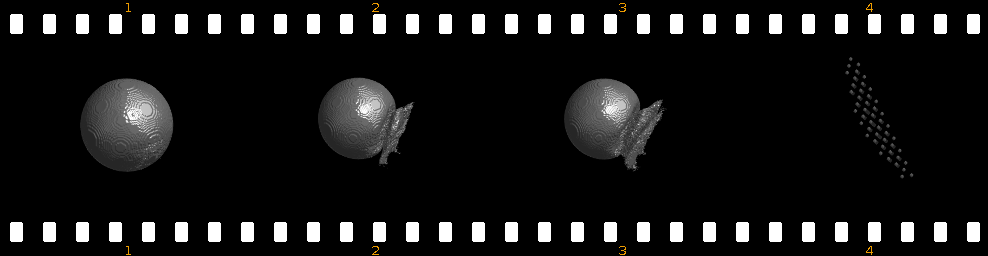
\includegraphics[width=.6\linewidth]{figures/object_recon/strips/rock_s3d.png} \\
    (a) \\
    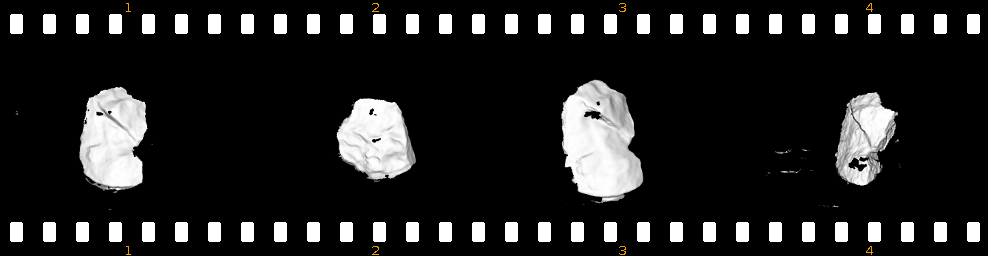
\includegraphics[width=.6\linewidth]{figures/object_recon/strips/rock.png} \\ 
    (b)\\
  \end{tabular}
  \caption[Probabilistic Object Reconstruction Qualitative Results I]
  {(a) The system of \textit{Ren et al} \cite{Ren2013} evolving a shape prior SDF 
  from RGBD observations on the Museum Rock sequence. (b) The proposed system reconstructing 
  the same object from observations of the Museum Rock sequence.}
\end{figure}

As can be observed in Figure \ref{fig:probobj_rock_s3d}, the proposed system of 
\textit{Ren et al} begins with a discretised SDF shape prior of a sphere that is 
evolved over time whilst simultaneously optimising for pose. However, it is evident 
that through the course of the sequence it is unable to evolve sufficiently to model 
the object of interest, contary to the approach outlined in this chapter.

\begin{figure}[h]
  \label{fig:probobj_dino_s3d}
  \centering
  \begin{tabular}{@{}c@{}}
    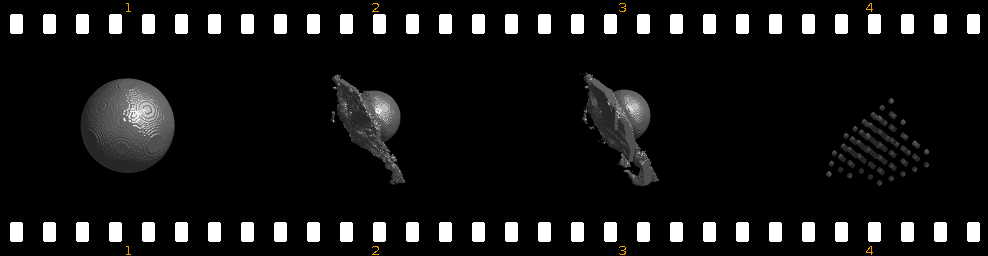
\includegraphics[width=.6\linewidth]{figures/object_recon/strips/dino_s3d.png} \\
    (a) \\
    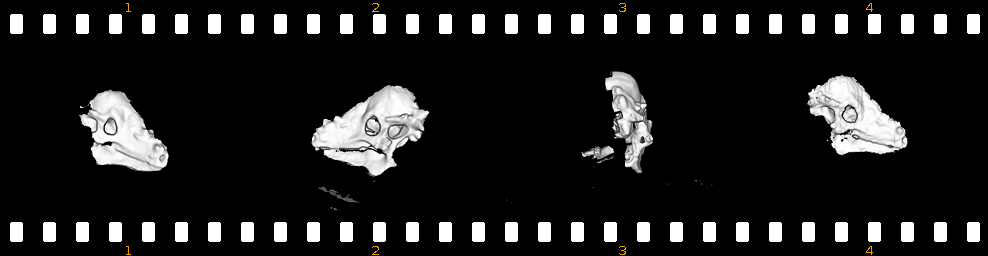
\includegraphics[width=.6\linewidth]{figures/object_recon/strips/dino.png} \\ 
    (b) \\
  \end{tabular}
  \caption[Probabilistic Object Reconstruction Qualitative Results II]
  {(a) The system of \textit{Ren et al} \cite{Ren2013} evolving a shape prior SDF 
  from RGBD observations on the Museum Dinosaur Head sequence. (b) The proposed system 
  reconstructing same the object from observations of the Museum Dinosaur Head sequence.}
\end{figure}

As with the example given in Figure \ref{fig:probobj_rock_s3d}, it can be seen in 
Figure \ref{fig:probobj_dino_s3d} that the system of \textit{Ren et al} is again 
unable to evolve the SDF shape prior suffiently to model the object of interest. As 
can be observed, again the proposed system of this work is capable of yielding a suitable 
reconstruction.

An additional evaluation is performed on the proposed systems ability to reconstruct 
a range of objects versus that of an implementation of the standard KinectFusion 
pipeline as outlined in Section \ref{MOSEG INTRO}. The central difference in the use 
of the two approaches for the purposes of this comparison is that in the proposed system, 
only the observed points of the live frame and of the reconstruction that belong to the 
object of interest are used for pose estimation. In the KinectFusion pipeline used 
as a base of comparison however, the entire scene is modelled as the camera is moved, 
with the reconstruction of the object of interest being segmented as a post processing 
step. As such, the results extracted from the KinectFusion pipeline are taken to be the 
ground truth reconstructions of the object of interest. This is due to the more robust 
pose estimation that would be expected from utilising all available geometric data 
for tracking, versus utilising only that of a single, potentially small object.

\begin{figure}[h]
  \label{fig:probobj_comp_itm}
  \centering
  \begin{tabular}{cccc}
    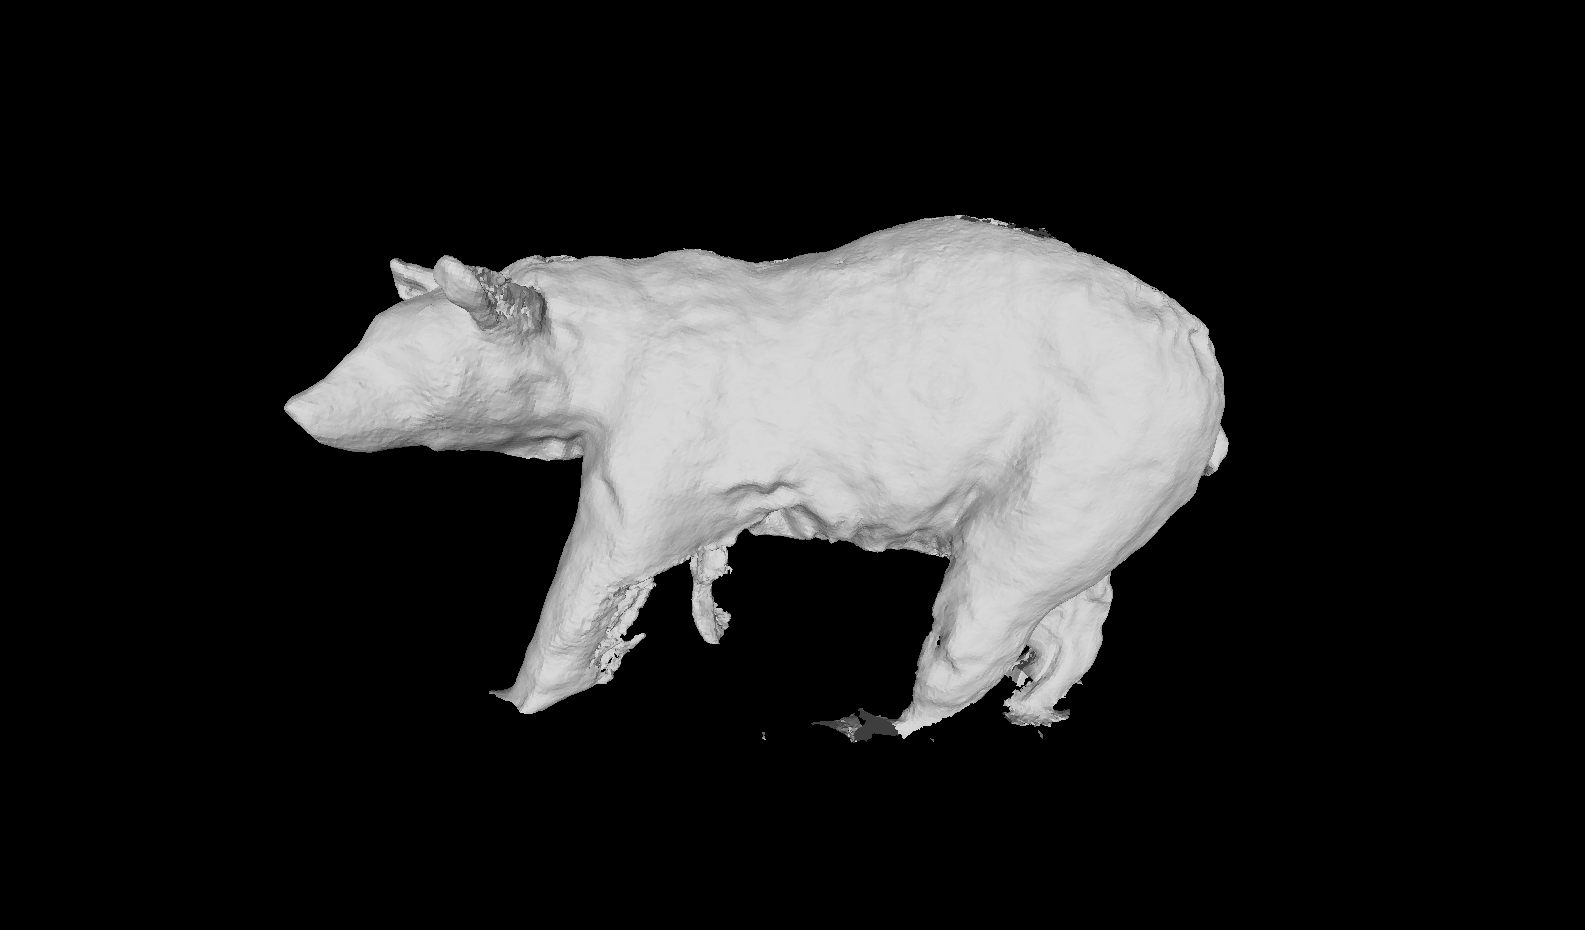
\includegraphics[width=.2\linewidth]{figures/object_recon/comp/itm/bear00.png}&
		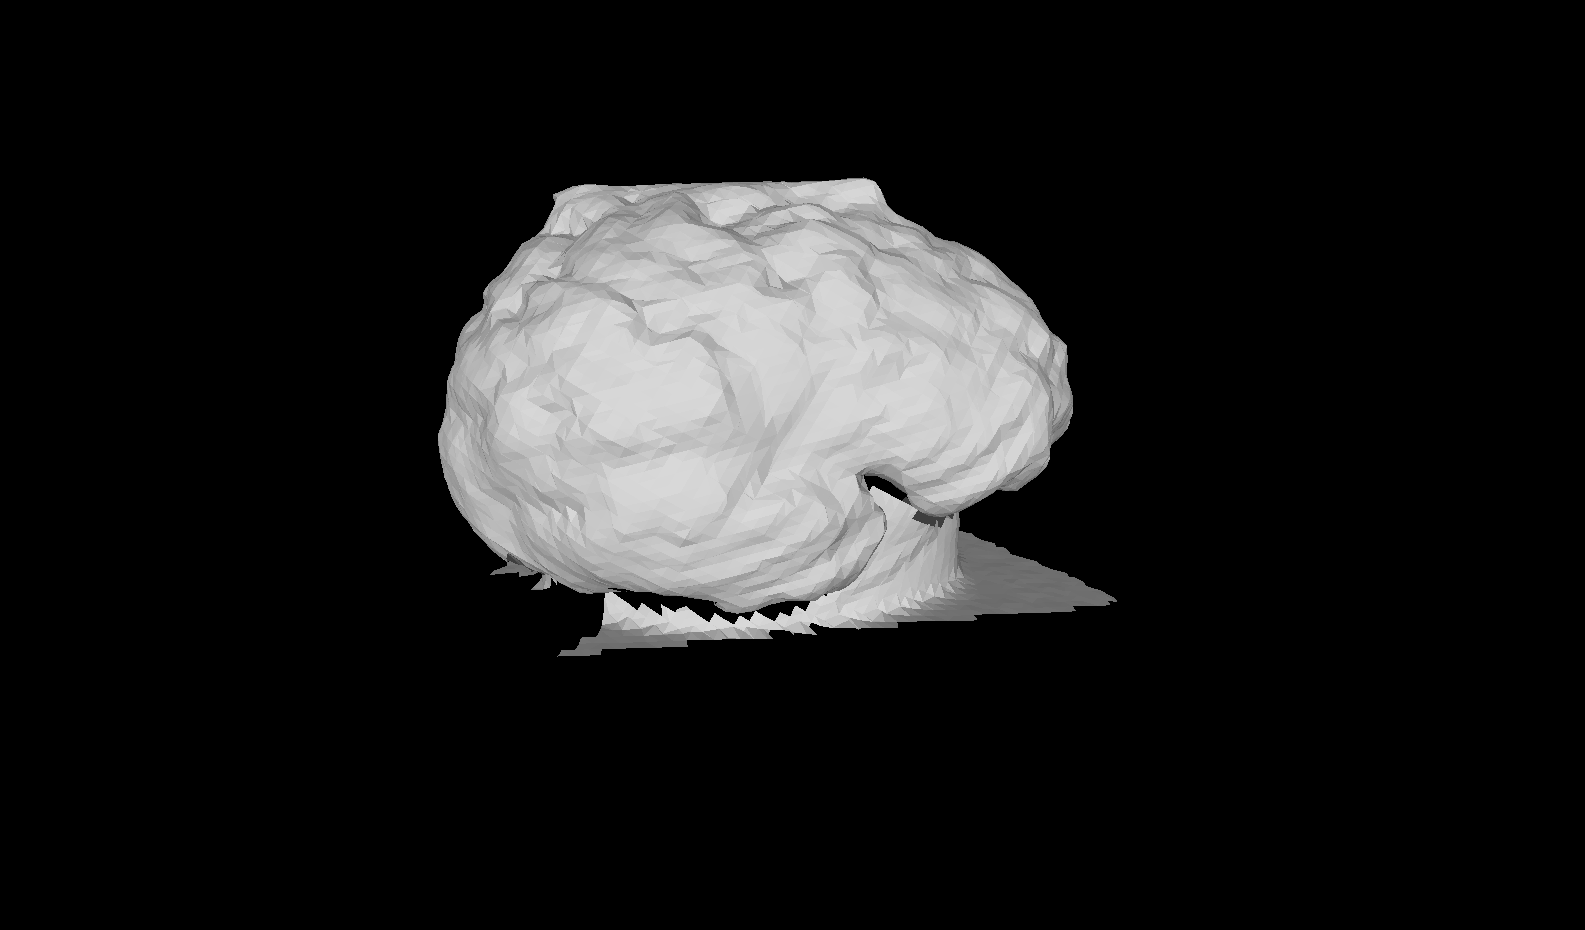
\includegraphics[width=.2\linewidth]{figures/object_recon/comp/itm/brain00.png}&
		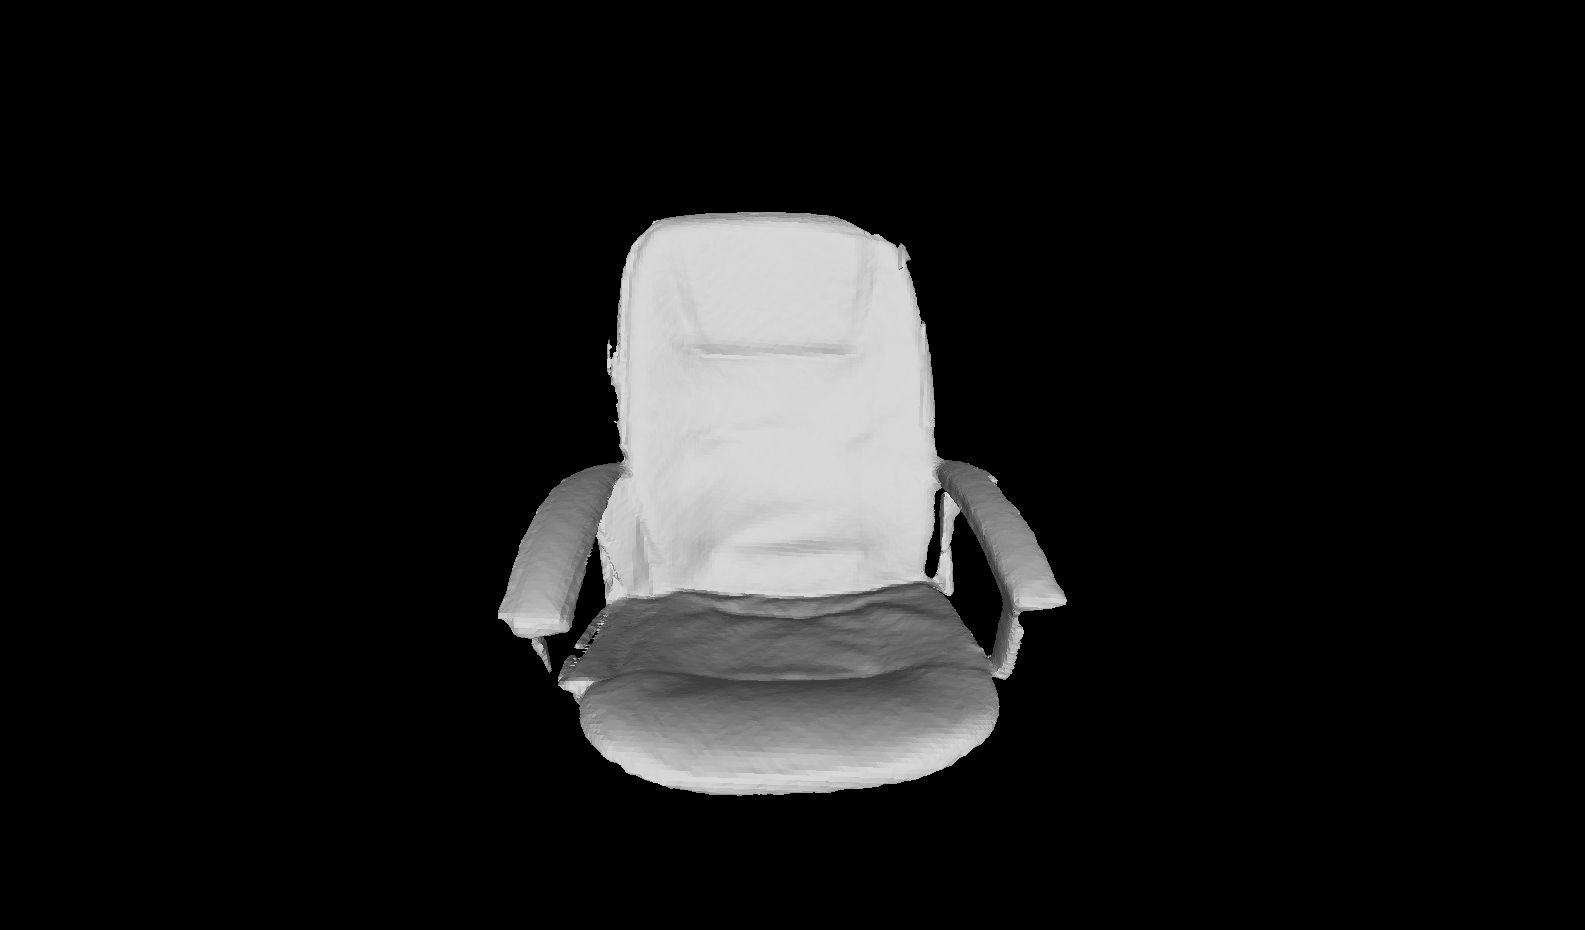
\includegraphics[width=.2\linewidth]{figures/object_recon/comp/itm/chair00.png}&
    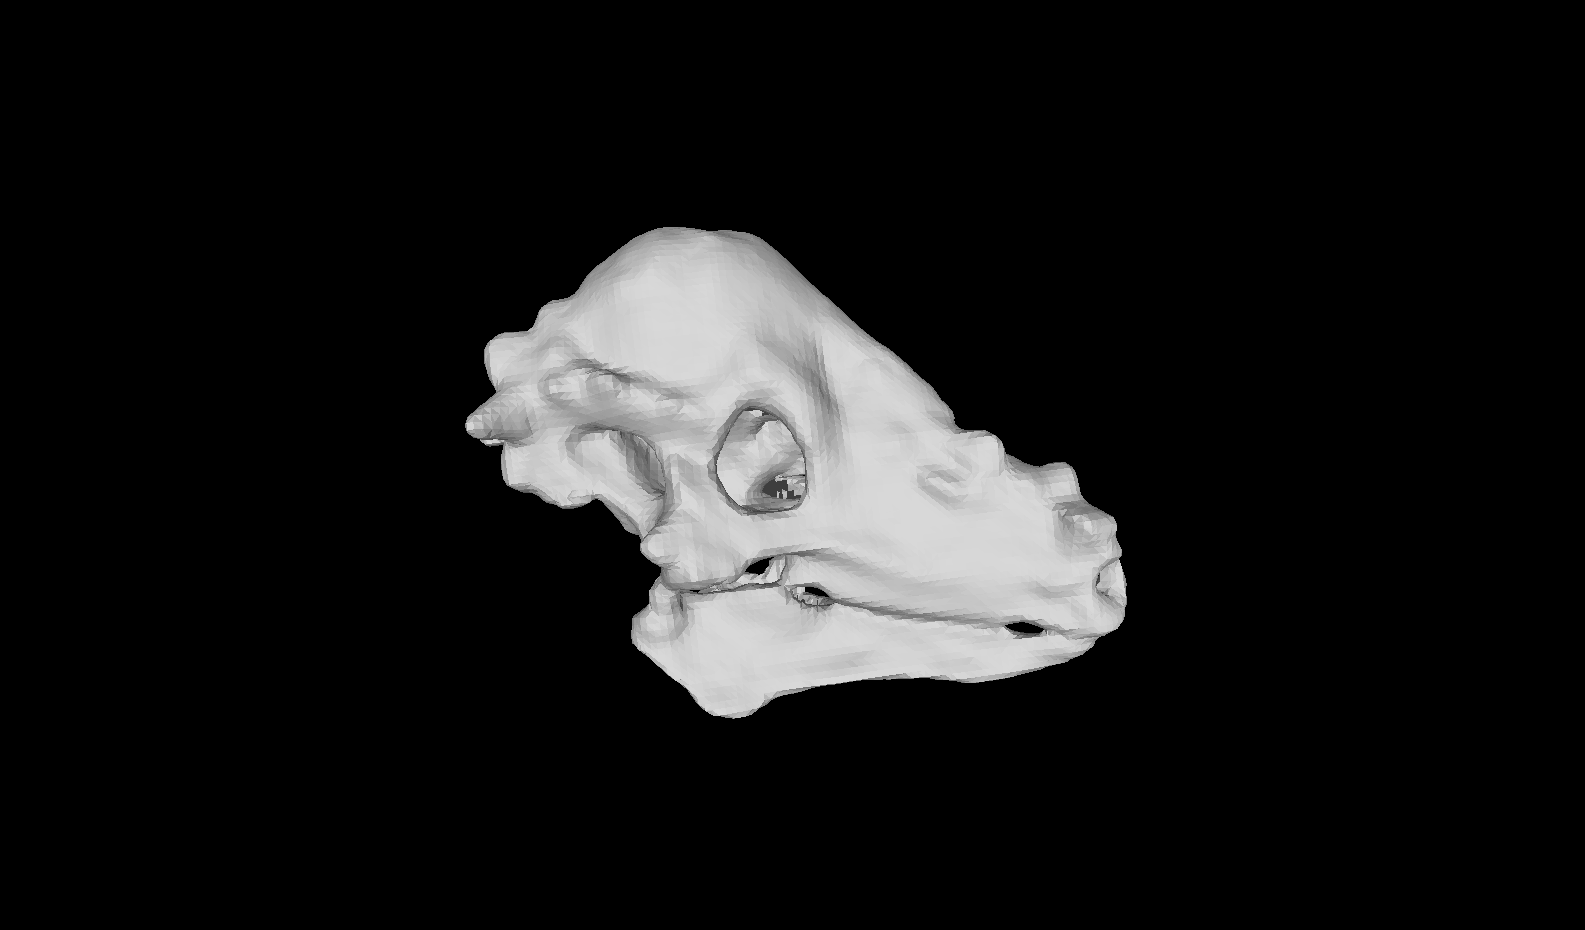
\includegraphics[width=.2\linewidth]{figures/object_recon/comp/itm/dino00.png} \\
    (a) & (b) & (c) & (d) \\
		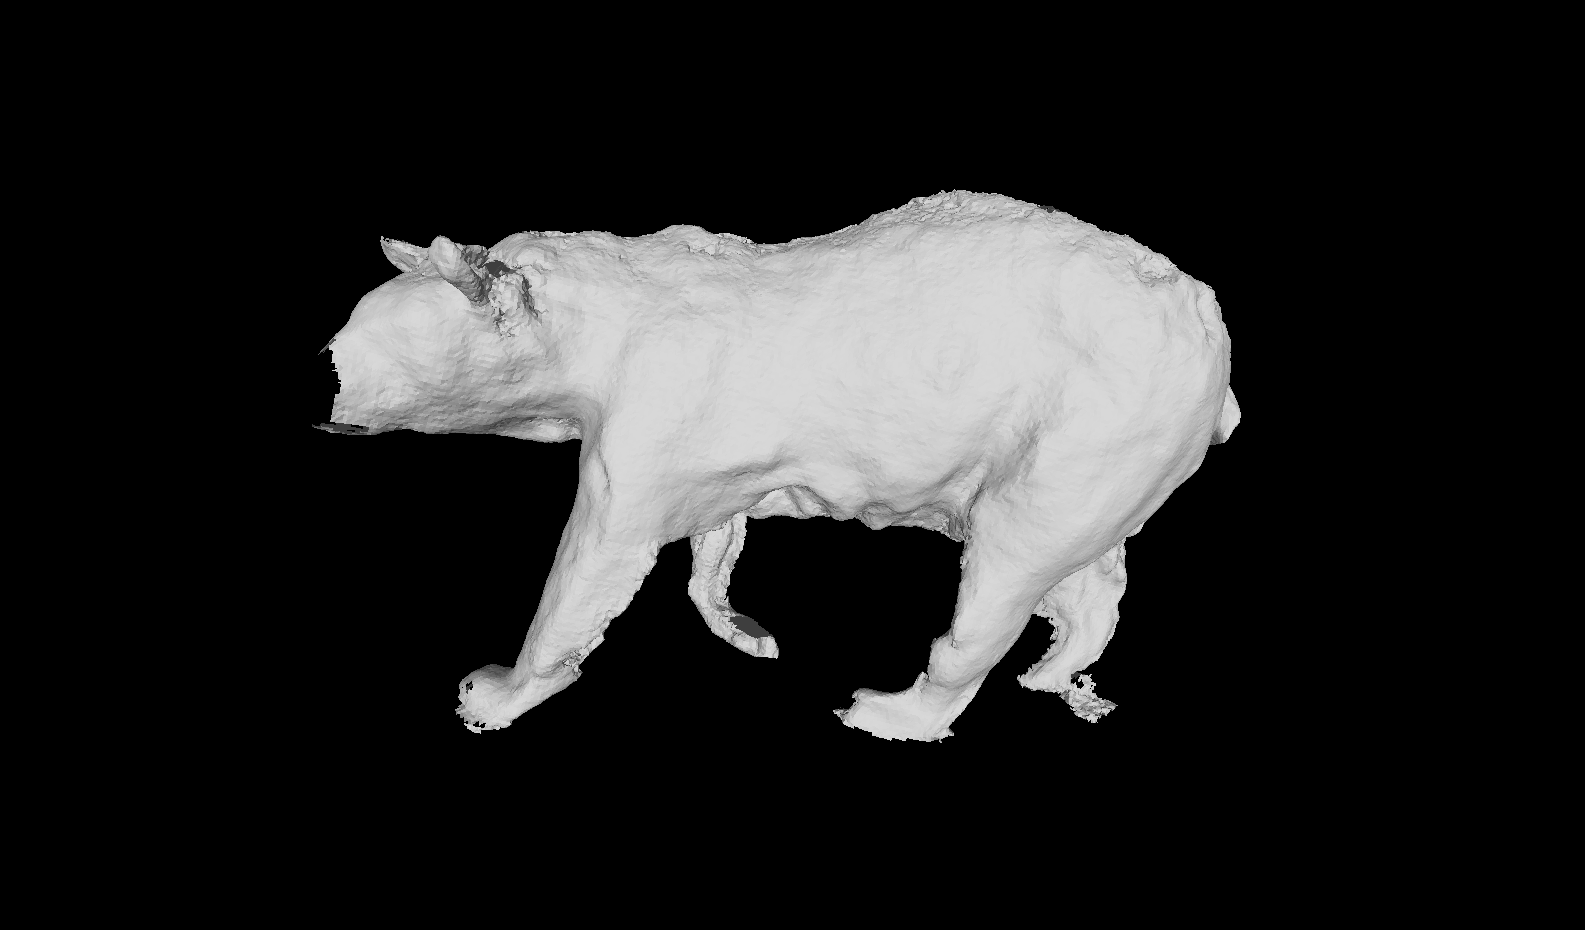
\includegraphics[width=.2\linewidth]{figures/object_recon/comp/prob/bear00.png}&
		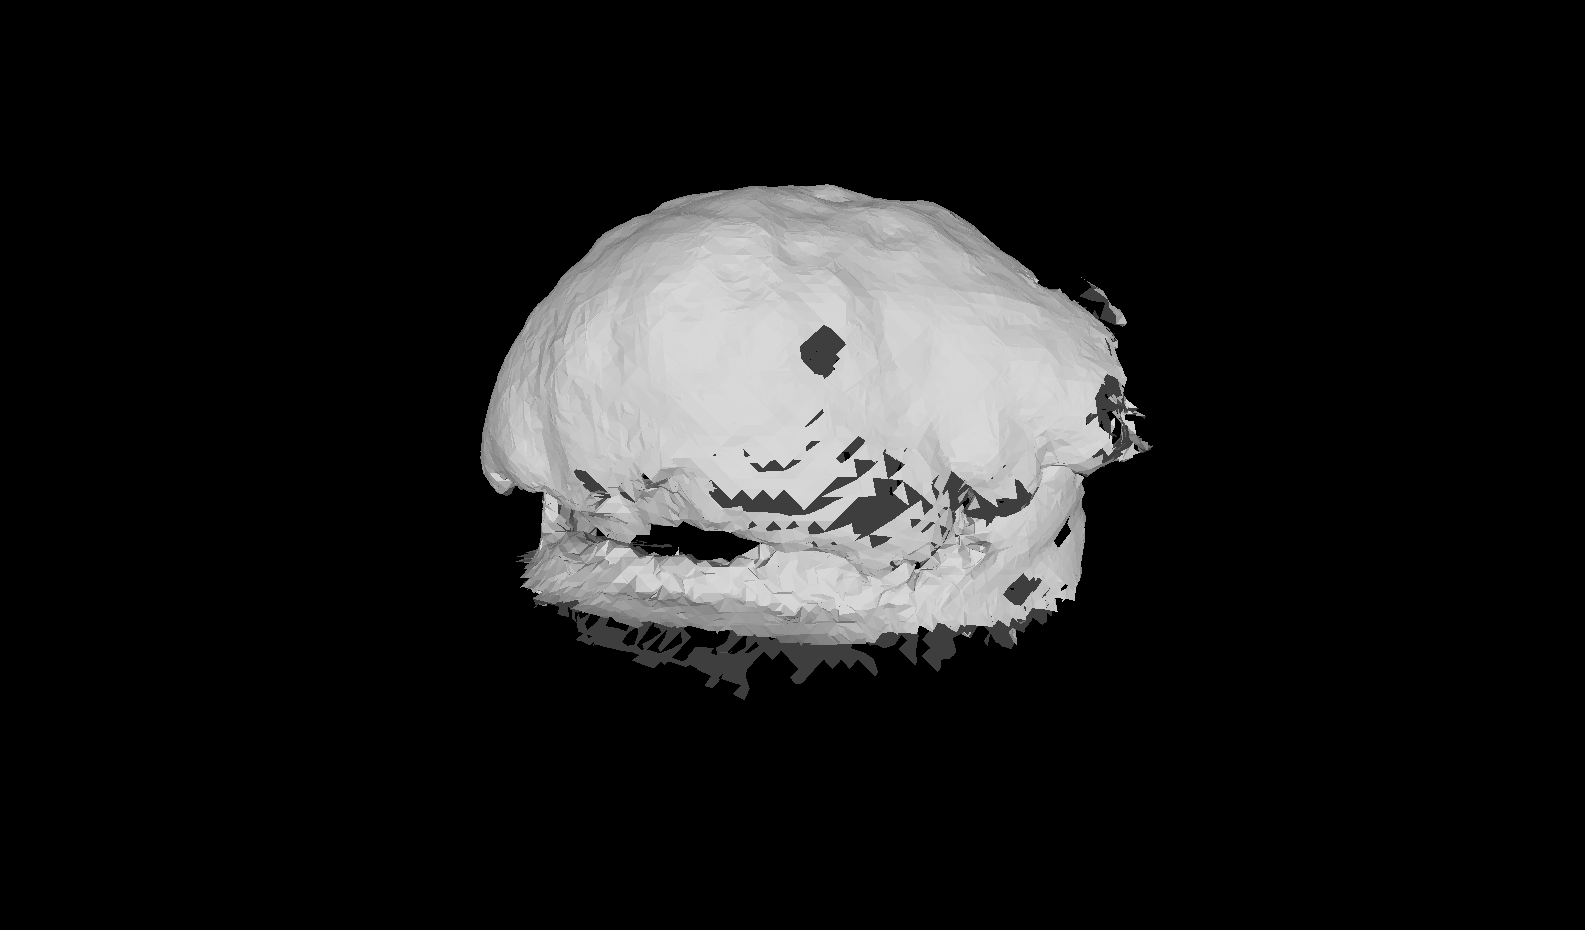
\includegraphics[width=.2\linewidth]{figures/object_recon/comp/prob/brain00.png}&
		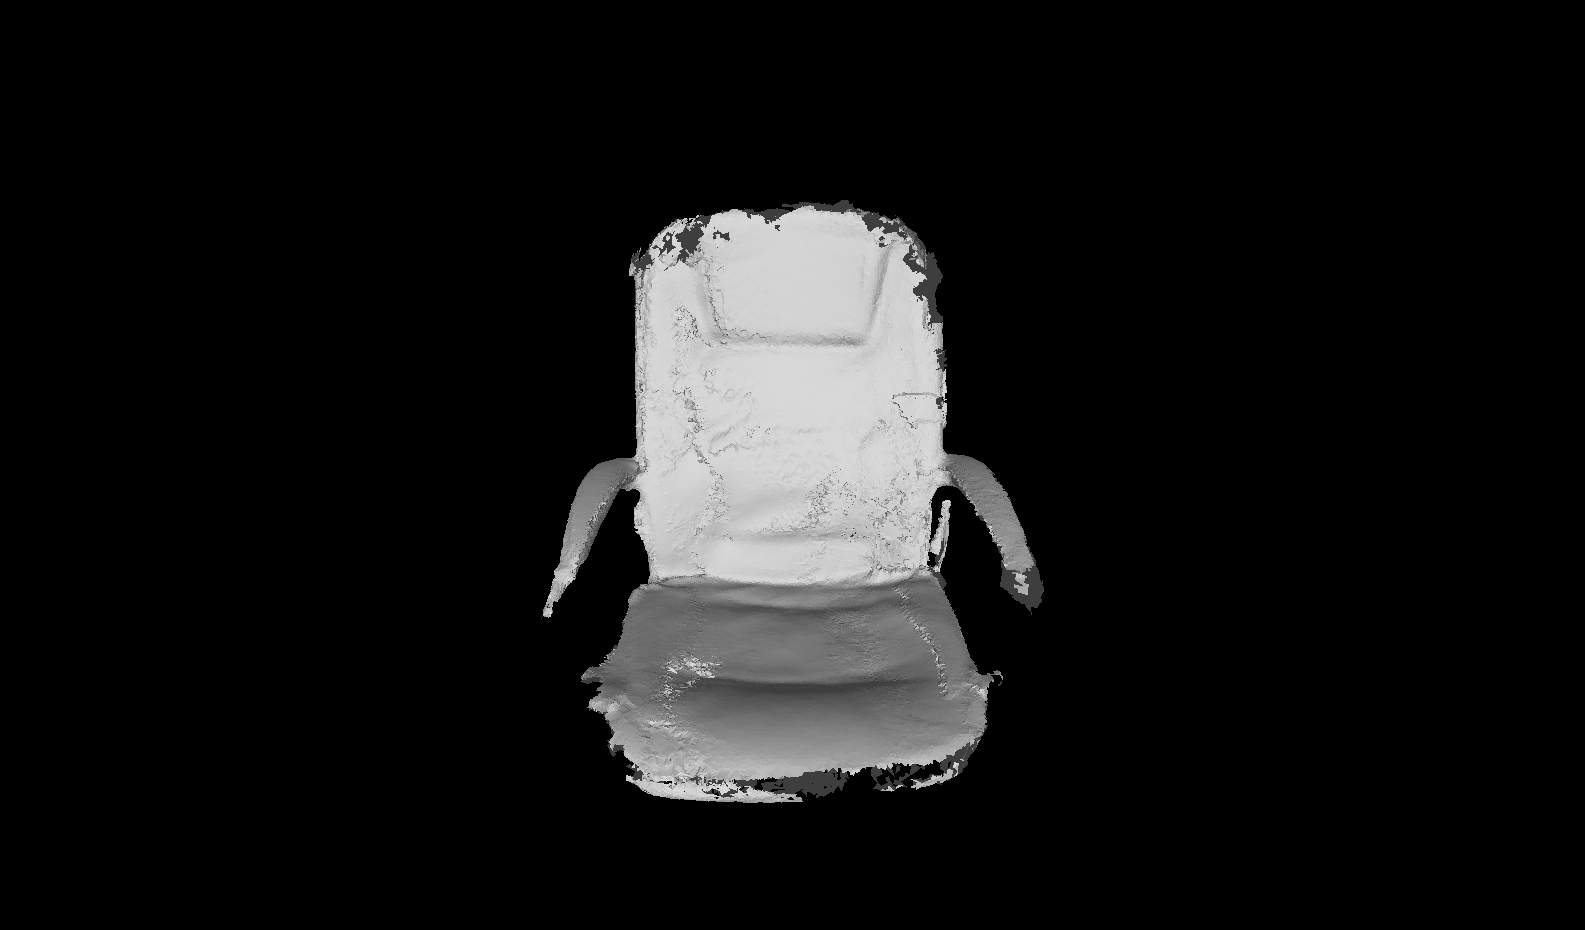
\includegraphics[width=.2\linewidth]{figures/object_recon/comp/prob/chair00.png}&
    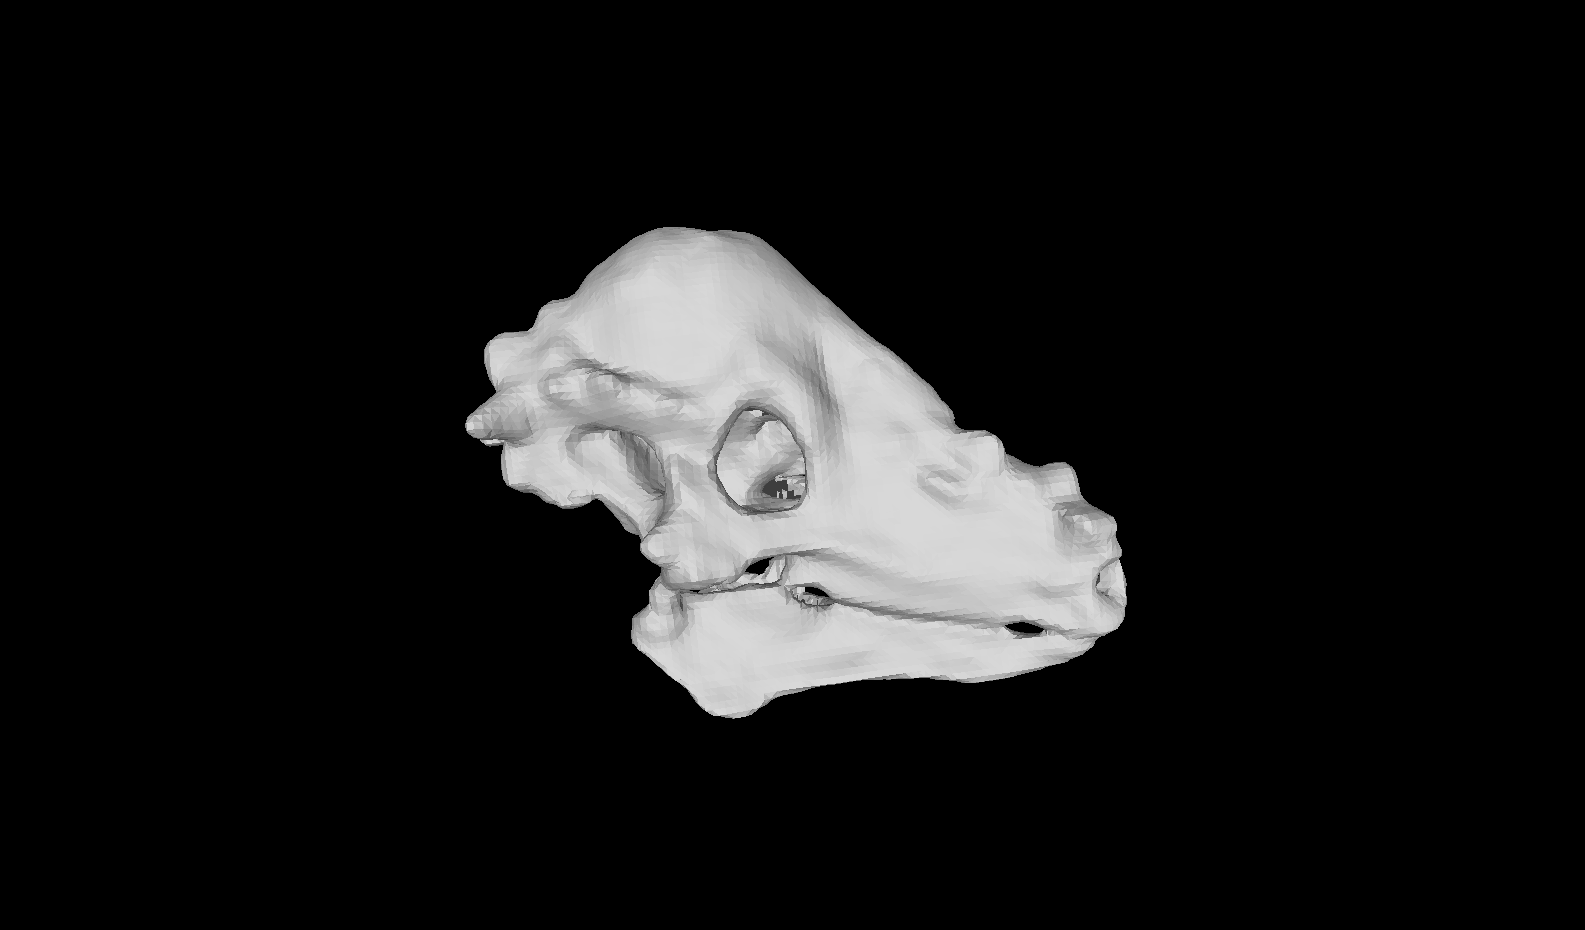
\includegraphics[width=.2\linewidth]{figures/object_recon/comp/itm/dino00.png} \\
    (e) & (f) & (g) & (h) \\
  \end{tabular}
  \caption[Probabilistic Object Reconstruction Qualitative Results III]
  {(a, b, c, d) Base reconstructions extracted from the output of the 
  standard KinectFusion pipeline. (e, f, g, h) Reconstructions yielded by 
  the proposed approach.}
\end{figure}

As can be seen in Figure \ref{fig:probobj_comp_itm} the proposed system is 
capable of providing reconstructions of a wide variety of objects in an 
aesthetically similar manner to a well established baseline. The proposed 
system provides globally consistent, closed reconstructions as is evident from 
the top-down views presented in Figure \ref{fig:probobj_comp_itm}.

\begin{figure}[h]
  \label{fig:probobj_comp_itm}
	\centering
	\begin{tabular}{cccc}
		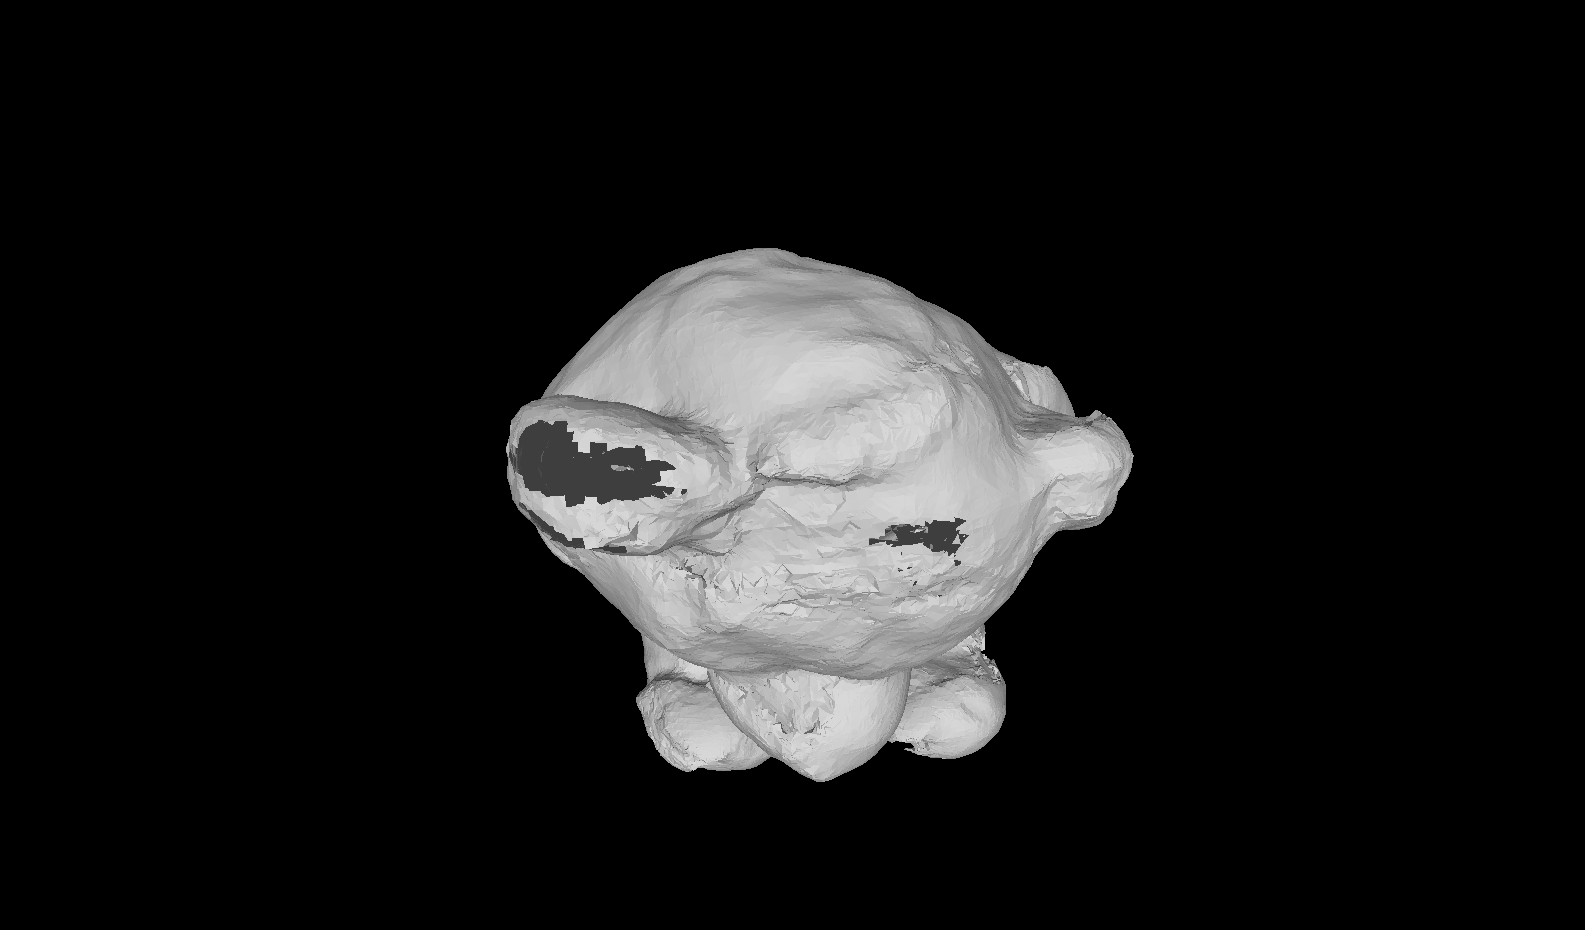
\includegraphics[width=.2\linewidth]{figures/object_recon/top/teddy_top00.png}&
    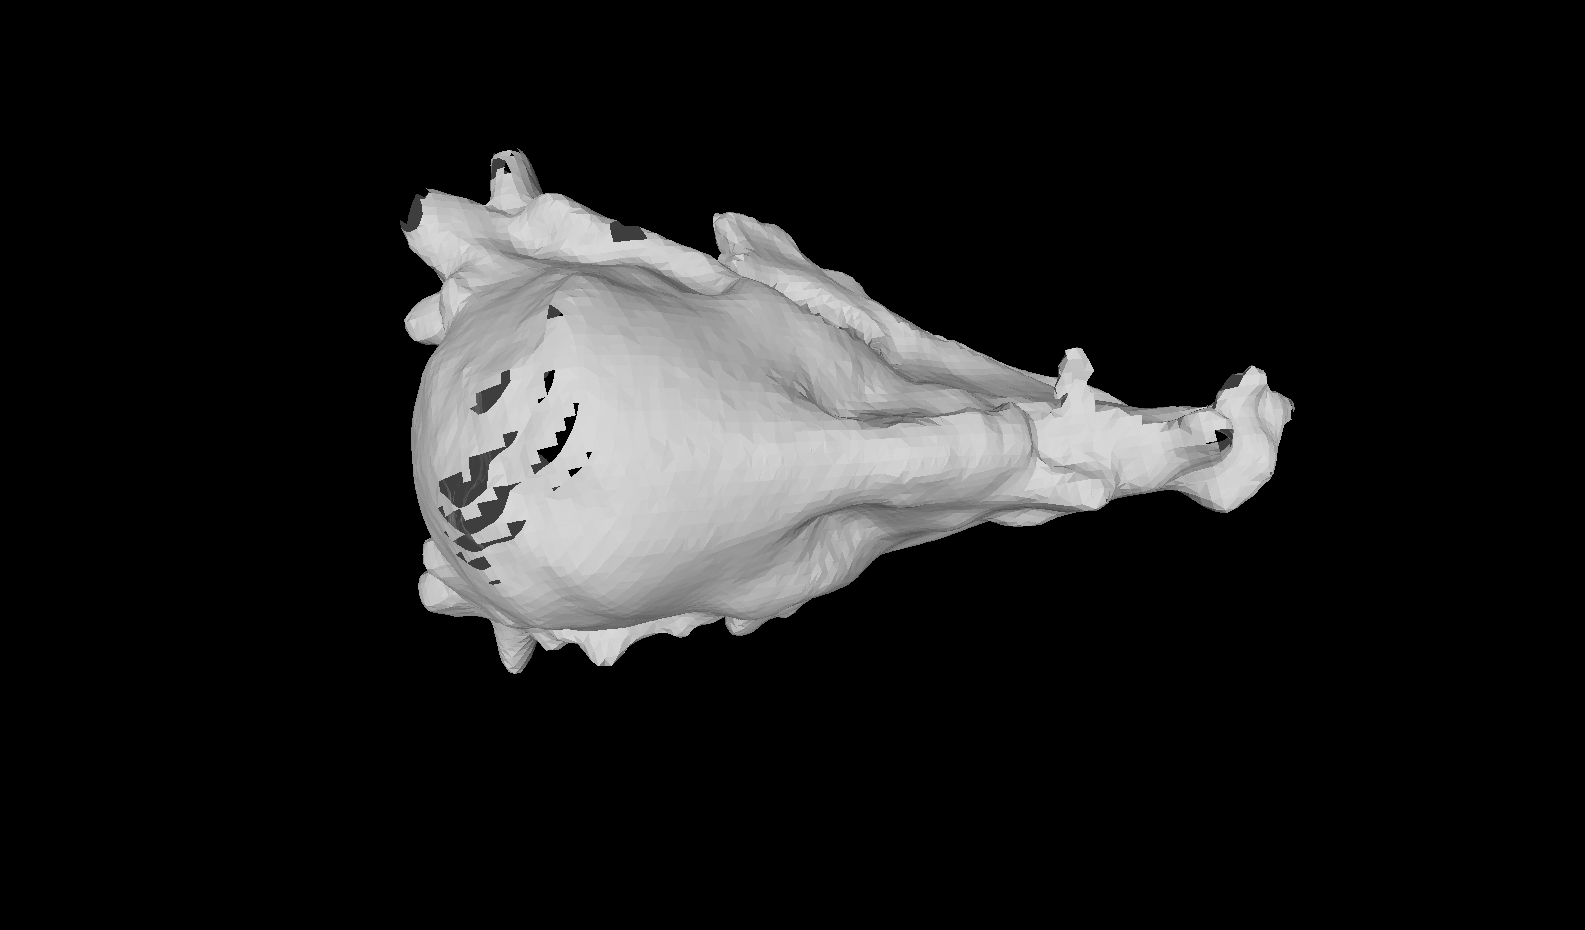
\includegraphics[width=.2\linewidth]{figures/object_recon/top/dino_top00.png} &
		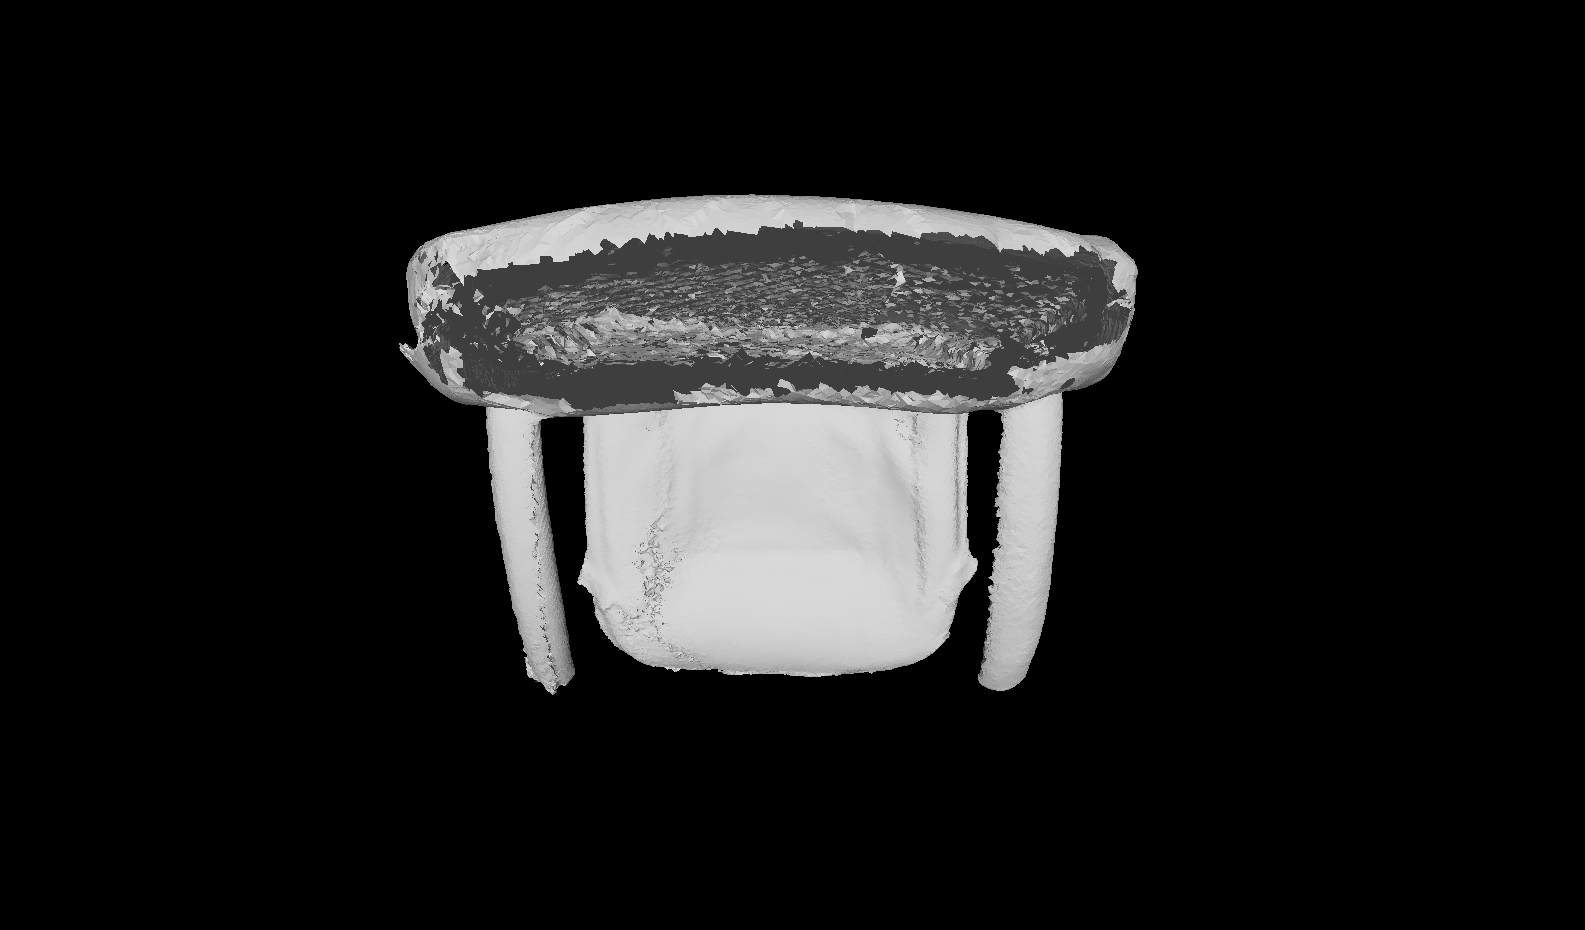
\includegraphics[width=.2\linewidth]{figures/object_recon/top/chair_top00.png}&
    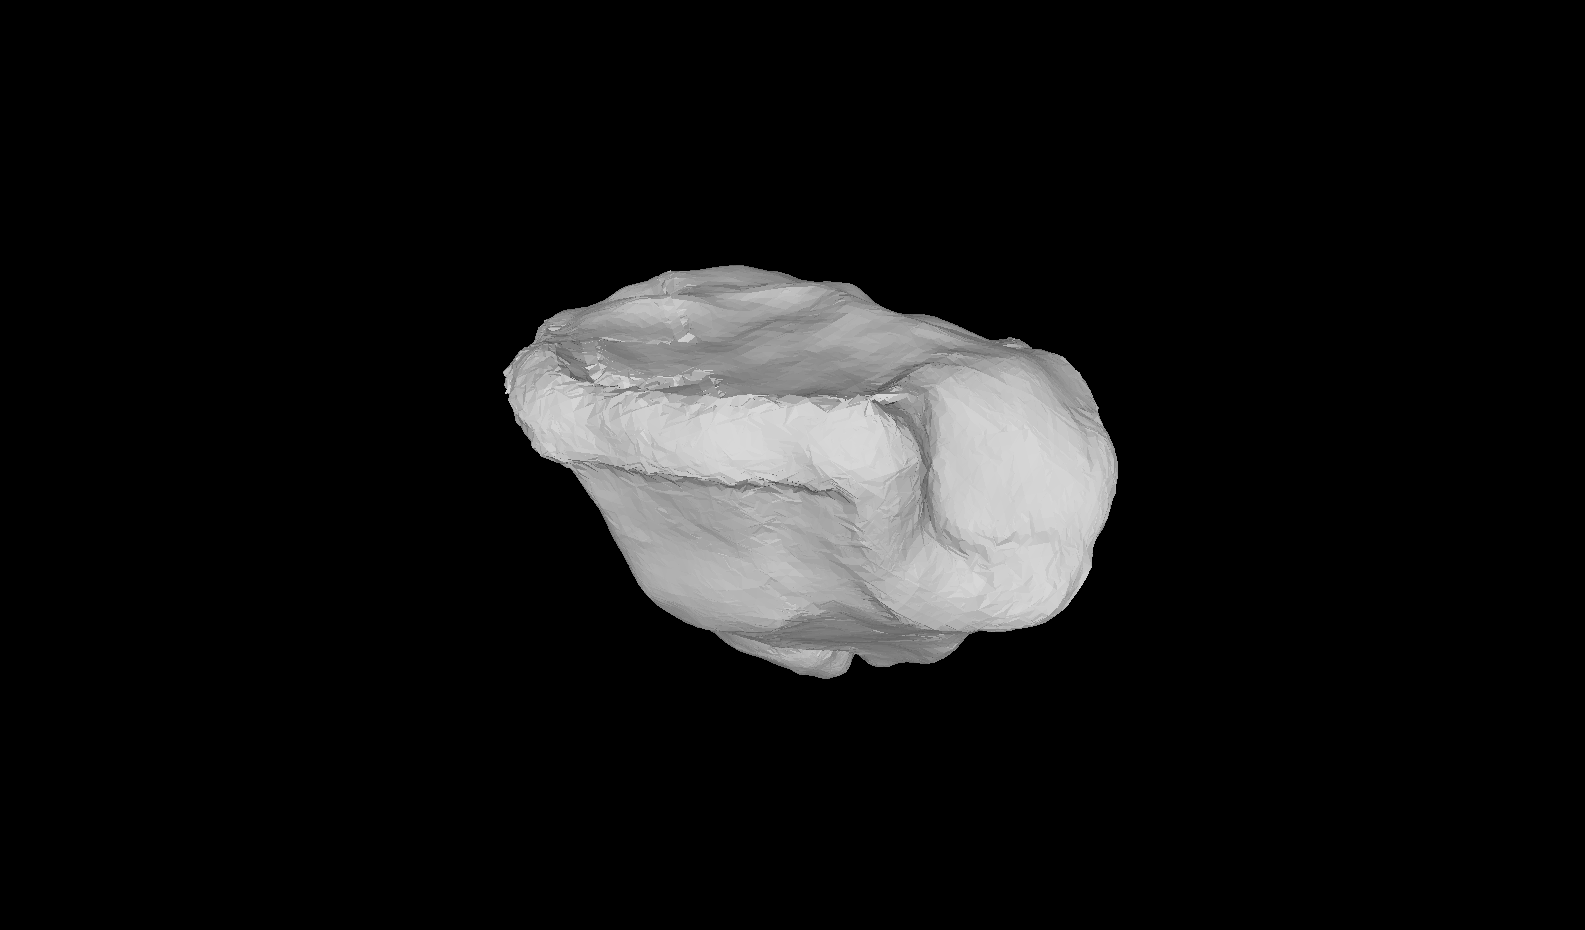
\includegraphics[width=.2\linewidth]{figures/object_recon/top/rock_top00.png} \\
    (a) & (b) & (c) & (d) \\
	\end{tabular}
  \caption[Probabilistic Object Reconstruction Qualitative Results IV]
  {
    Closed reconstructions of the (a) Teddy, (b) Dinosaur Head, 
    (c) Chair and (d) Rock sequences.
	}
\end{figure}

The efficacy of the approach described in this work is further demonstrated when comparing
the pipeline as outlined in Figure \ref{fig:probobj_pipeline_diagram} to a version that 
utilises only a single representation of the object of interest. Figure 
\ref{fig:probobj_gappy_teddy} demonstrates the difference in reconstruction output when 
not utilising the multiple subvolume representation and it's accompanying enforcement 
of consistency constraints. 

\begin{figure}[h]
  \label{fig:probobj_gappy_teddy}
	\centering
	\begin{tabular}{cc}
		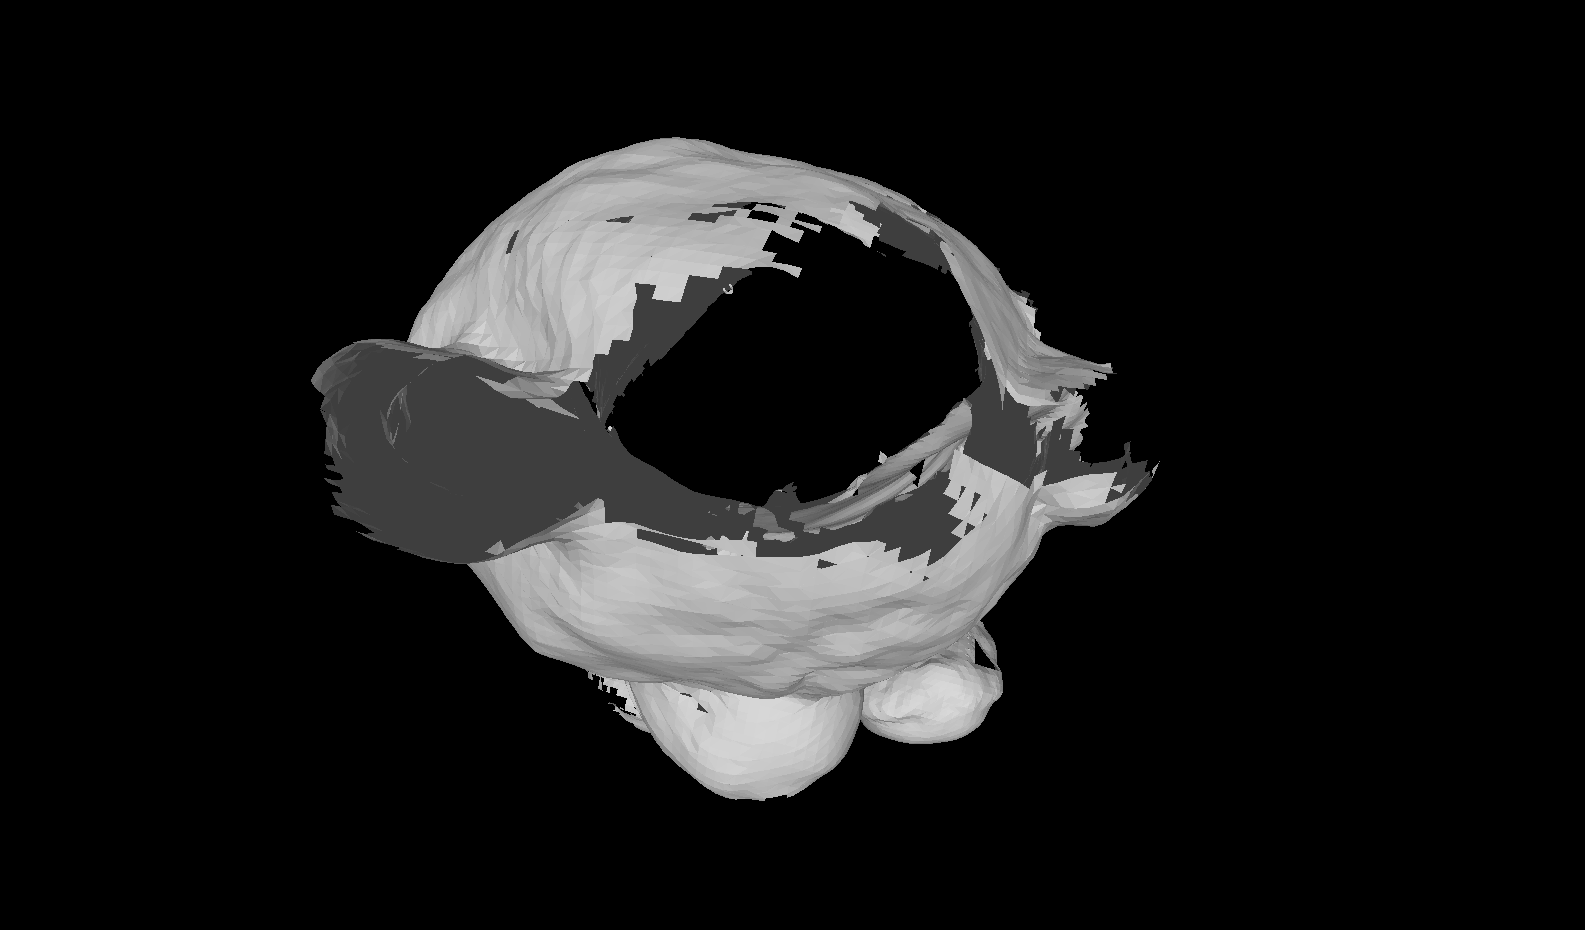
\includegraphics[width=.2\linewidth]{figures/object_recon/gappy/one_scene00.png}&
    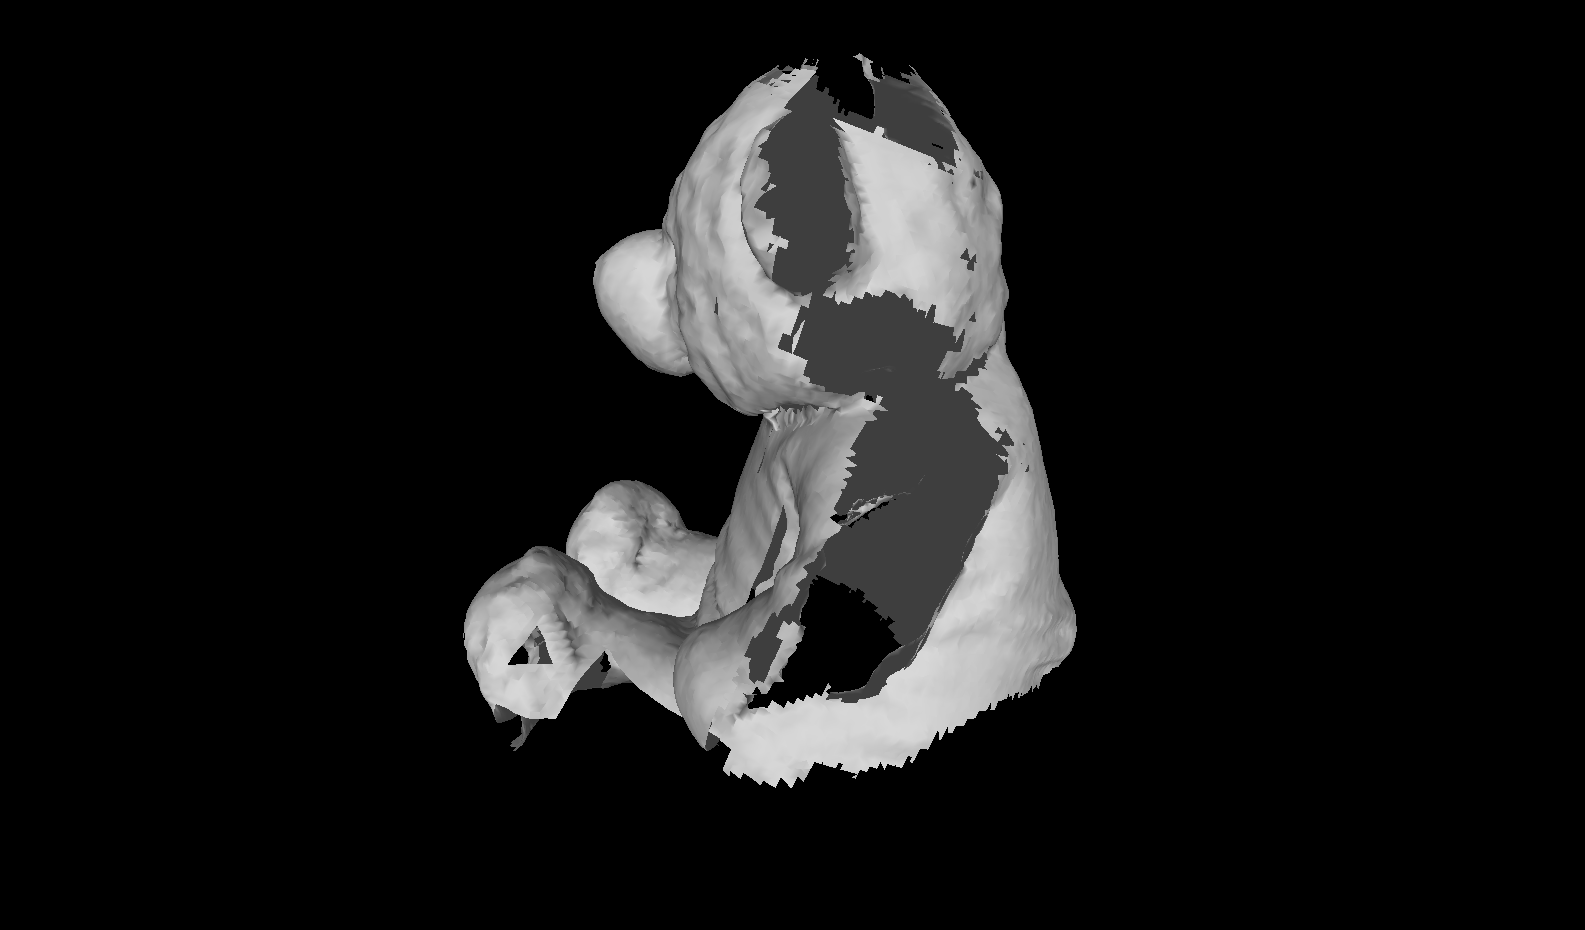
\includegraphics[width=.2\linewidth]{figures/object_recon/gappy/one_scene01.png}\\
    (a) & (b) \\
		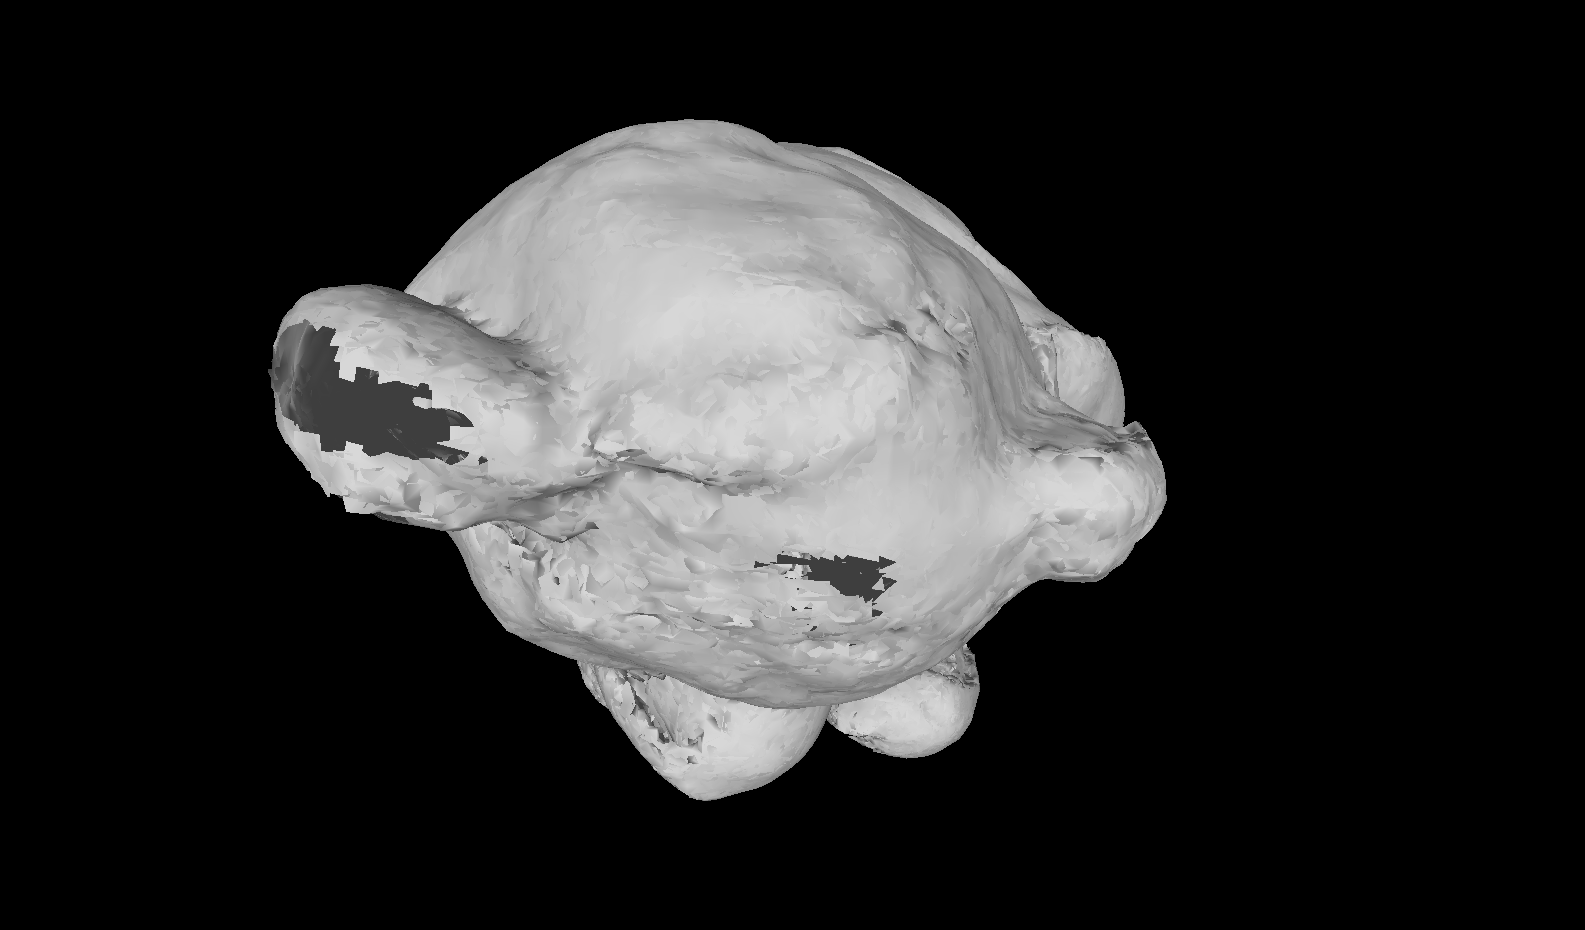
\includegraphics[width=.2\linewidth]{figures/object_recon/gappy/multi_scene00.png}&
    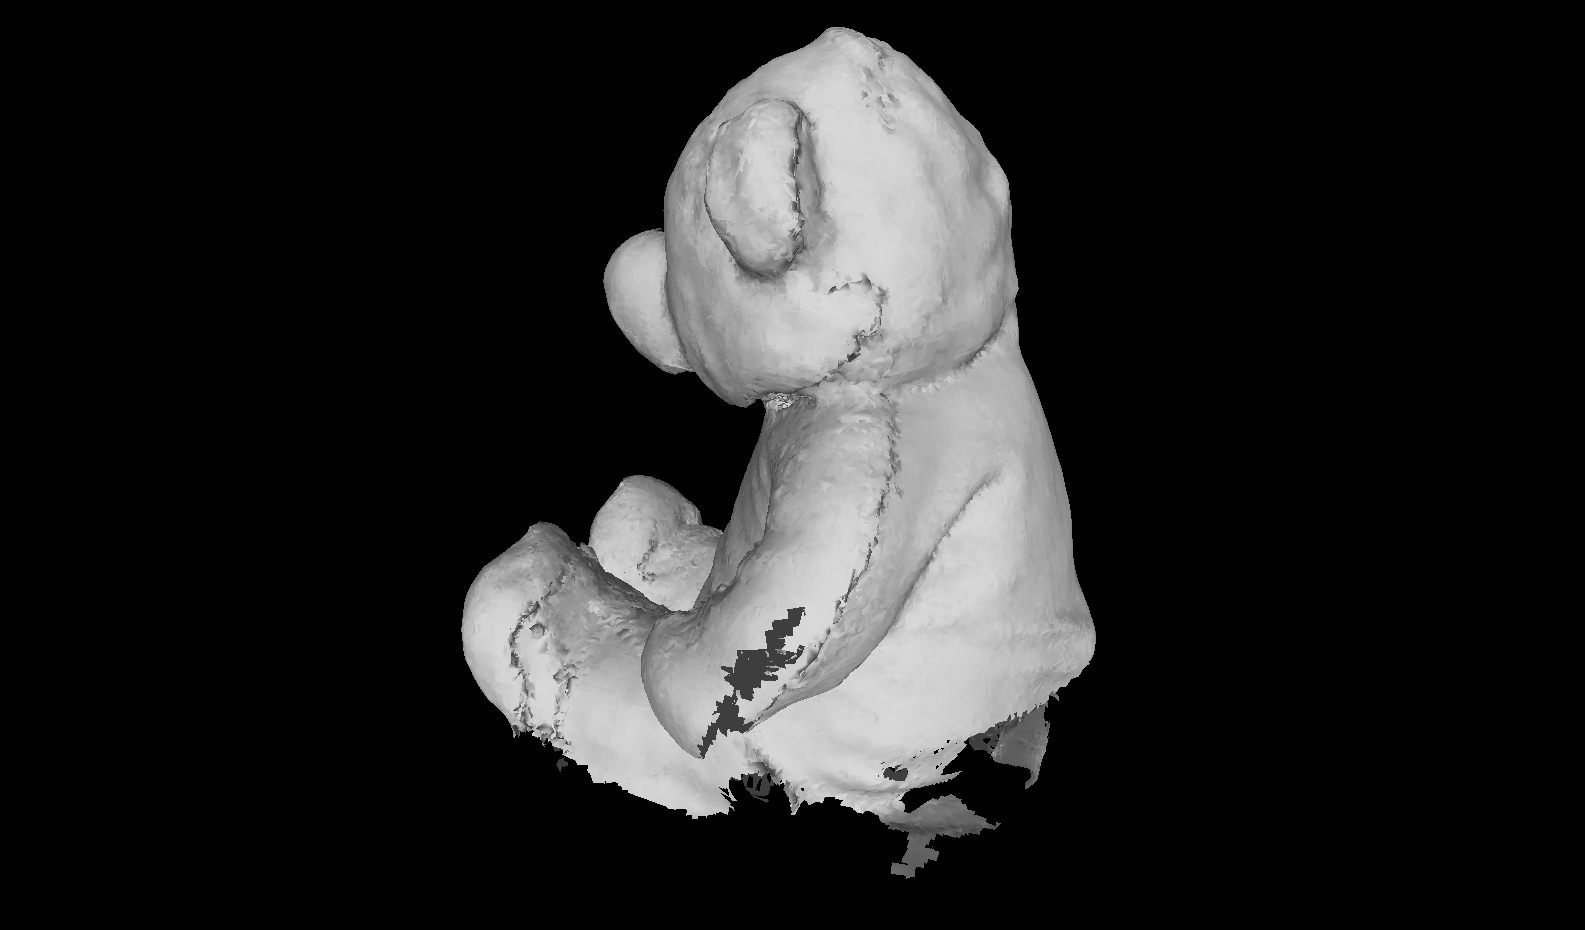
\includegraphics[width=.2\linewidth]{figures/object_recon/gappy/multi_scene01.png}\\
    (c) & (d)\\
	\end{tabular}
  \caption[Probabilistic Object Reconstruction Qualitative Results V]
  {
    Teddy reconstruction with InfiniTAM (a, b) versus the system proposed in this 
    work (c, d).
	}
\end{figure}

The gaps in the isosurface depicted in Figure \ref{fig:probobj_gappy_teddy} (a, b) 
demonstrate the impact that drift in the pose estimation stage can have on the resultant 
reconstruction; drift can incur irregularities in the extraction and rendering of the objects 
isosurface. Note that the reconstructions given in Figure \ref{fig:probobj_gappy_teddy} 
(c, d) do not suffer such irregularities when utilising the object reconstruction pipeline 
presented in this chapter.

\section{Quantitative Results}
\label{sec:probobj_quantitative}
In this section the performance of the proposed system is evaluated quantitatively with respect 
to both pose estimation accuracy and reconstruction accuracy. 

For pose evaluation, the \textit{3D Object Reconstruction} subset of the 
\textit{RGB-D SLAM Dataset and Benchmark} \cite{Sturm2012}. The objects of interest in 
the dataset vary largely in both geometry and appearance. As with the quantitative 
evaluation presented in Section \ref{sec:moseg_quantitative}, the 
\textit{Absolute Trajectory Error} is the primary metric of interest.

\begin{table}[h]
  \label{tbl:probobj_ate}
  \centering
  \begin{tabular}{l@{\hskip 1cm} c c}
    \emph{Sequence Name} & \emph{Proposed Approach ATE (m)} & \emph{InfiniTAM (m)}\\
    \midrule
    \textsf{freiburg3\_cabinet} & 0.077903 & 0.520693\\
    \textsf{freiburg3\_teddy}   & 0.030596 & 0.048560 \\
    \textsf{freiburg1\_plant}   & DNR & DNR \\
    \textsf{freiburg2\_coke}   & DNR & DNR \\
    \textsf{freiburg2\_dishes}   & DNR & DNR \\
    \textsf{freiburg2\_flowerbouquet}   & DNR & DNR \\
    \textsf{freiburg2\_flowerbouquet\_brownbackground}   & DNR & DNR \\
    \textsf{freiburg2\_metallic\_sphere}   & DNR & DNR \\
    \textsf{freiburg2\_metallic\_sphere2}   & DNR & DNR \\
    \textsf{freiburg3\_large\_cabinet}   & DNR & DNR
  \end{tabular}
  \caption[Probabilistic Object Reconstruction ATE]
  {ATE results achieved by the proposed approach versus InfiniTAM with object segmentation.}
\end{table}

It can be seen from Table \ref{tbl:probobj_ate} that on the \textit{freiburg3\_cabinet} 
and \textit{\textsf{freiburg3\_teddy}} sequences the approach proposed in this work 
yields a marked improvement in Absolute Trajectory Error over that of the standard KinectFusion 
pipeline with object segmentation. The remaining sequences that have the ATE marked as DNR did 
not yield an interpretable reconstruction; sequences with ATE metrics marked DNR did not 
reconstruct. In the case of the \textit{freiburg2\_metallic\_sphere(2)} sequences...

The trajectories of the two approaches evaluated on the \textit{freiburg3\_cabinet} 
and \textit{\textsf{freiburg3\_teddy}} sequences are plotted versus the ground truth trajectories 
in Figure \ref{fig:probobj_traj}

\begin{figure}[h]
  \label{fig:probobj_traj}
  \centering
  \begin{tabular}{cc}
  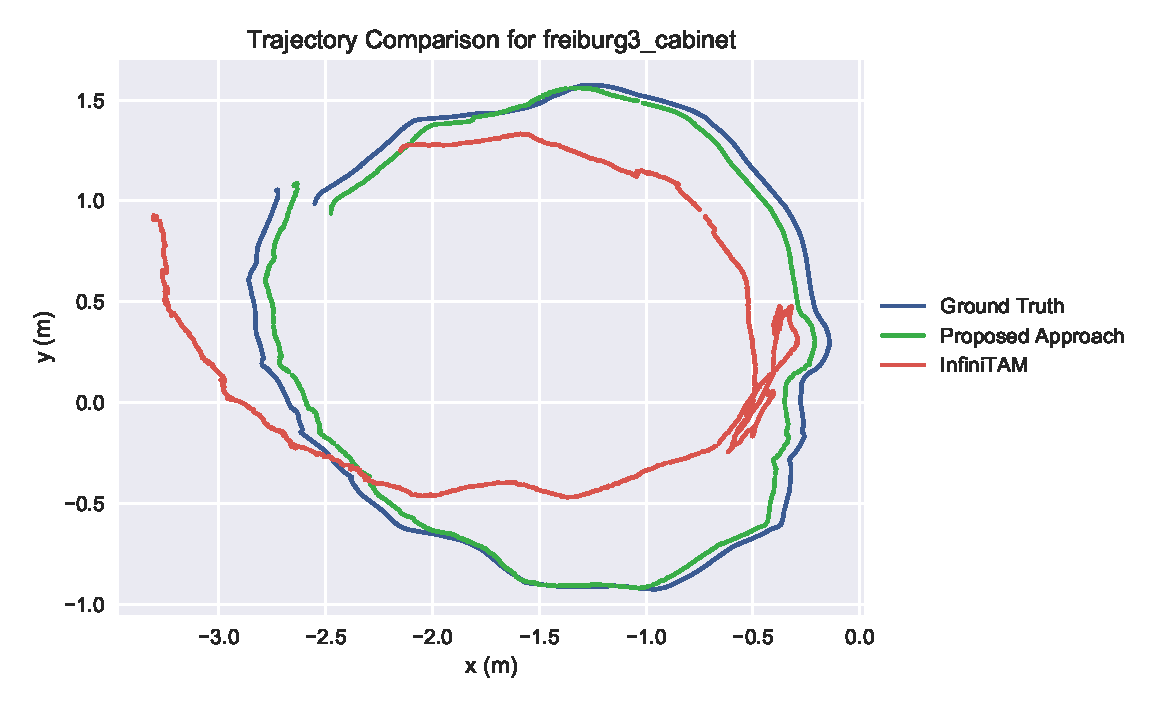
\includegraphics[width=.5\linewidth]{figures/object_recon/plots/traj/cab_traj.eps} & 
  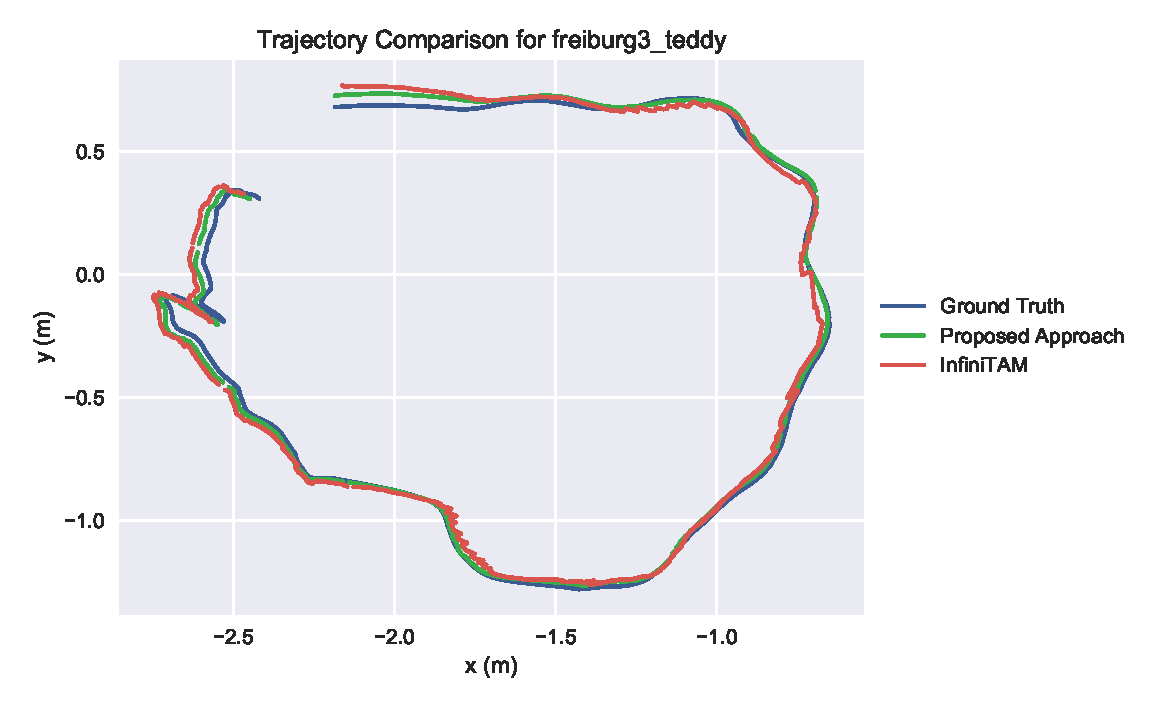
\includegraphics[width=.5\linewidth]{figures/object_recon/plots/traj/ted_traj.eps} \\
  (a) & (b)
  \end{tabular}
  \caption[Probabilistic Object Reconstruction Trajectory Plots]
  {Trajectory plots for the \textit{freiburg3\_cabinet} (a) 
  and \textit{\textsf{freiburg3\_teddy}} (b) sequences.}
\end{figure}

The proposed system is additionally evaluated quantitatively with respect to reconstruction 
quality. Reference models are obtained by reconstructing both the object of interest and it's 
surrounding scene (for maximal Pose Estimation accuracy), followed by a manual segmentation of 
the object of interest in 3-space. To quantify the reconstruction quality the Hausdorff 
Distance \cite{Hausdorff} for subsets of metric spaces is used, where in this case the metric 
space is Euclidean. The Hausdorff Distance is defined as follows in Equation \ref{eqn:probobj_hauss}
\begin{equation}
  \label{eqn:probobj_hauss}
  d_{H}(X, Y) = \max \Bigg[
  \sup_{x \in X} \inf_{y \in Y} d(x, y), \sup_{y \in Y} \inf_{x \in X} d(x, y) 
  \Bigg]
\end{equation}
In Equation \ref{eqn:probobj_hauss}, $X$ is the ground truth dense SLAM reconstruction, 
$Y$ is the reconstruction outputted by the proposed system and $d(.)$ is the Euclidean 
distance.

The resultant quantitative comparisons may be found in Table \ref{tbl:probobj_hauss}.
\begin{table}[h]
  \label{tbl:probobj_hauss}
  \centering
  \begin{tabular}{lcccc}
    \emph{Sequence} & \emph{Min Dist} & \emph{Max Dist} & \emph{Mean Dist} & \emph{RMS}\\
    \midrule
    \textsf{Bear} & 0 & 0.102777 & 0.013588 & 0.019796 \\
    \textsf{Brain} & 0 & 0.026465 & 0.008745 & 0.011349 \\
    \textsf{Chair} & 0 & 0.053441 & 0.012349 & 0.016422 \\
    \textsf{Dinosaur Head} & 0 & 0.035252 & 0.007919 & 0.010676
  \end{tabular}
  \caption[Probabilistic Object Reconstruction Hausdorff Distance]
  {Minimum, maximum, mean and RMSE distances between the reconstructions yielded by 
  the proposed system and the baseline.}
\end{table}

As can be seen by the similarity measures presented, the proposed system is capable of 
yielding reconstructions to a high quality despite the markedly more difficult pose estimation 
scenario of utilising the observations of a single object rather than those an entire scene. 
It can be seen that the presented output reconstructions are geometrically close to those 
reconstructed with a dense SLAM system \cite{Prisacariu2014} following the KinectFusion 
\cite{Newcombe2011} pipeline that is modelling and tracking the entire scene and thus has 
much more geometrical data with which to estimate pose.

Figure \ref{fig:probobj_hauss} presents renderings of the \textit{Teddy}, 
\textit{Brain}, \textit{Chair} and \textit{Dinosaur Head} sequences textured 
on the Haussdorf Distance between the output reconstructions of the presented 
system and the base reconstructions extracted from the KinectFusion like pipeline.

\begin{figure}[h]
  \label{fig:probobj_hauss}
  \centering
  \begin{tabular}{@{}c@{}}
    \begin{tabular}{cccc}
      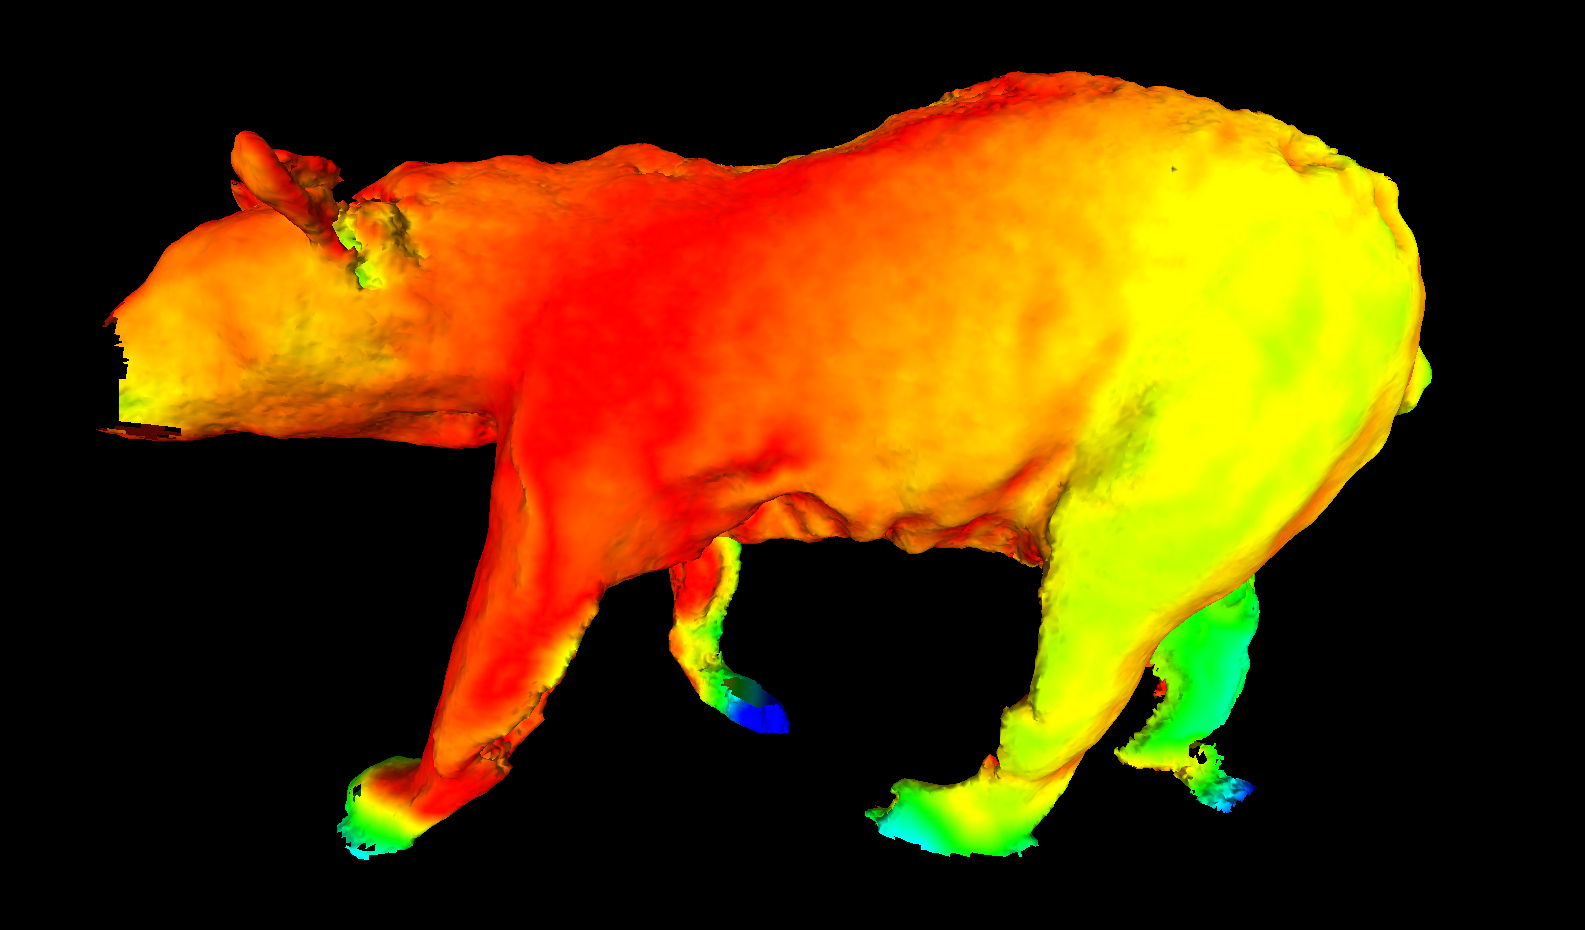
\includegraphics[width=.2\linewidth]{figures/object_recon/hauss/bear.png}&
      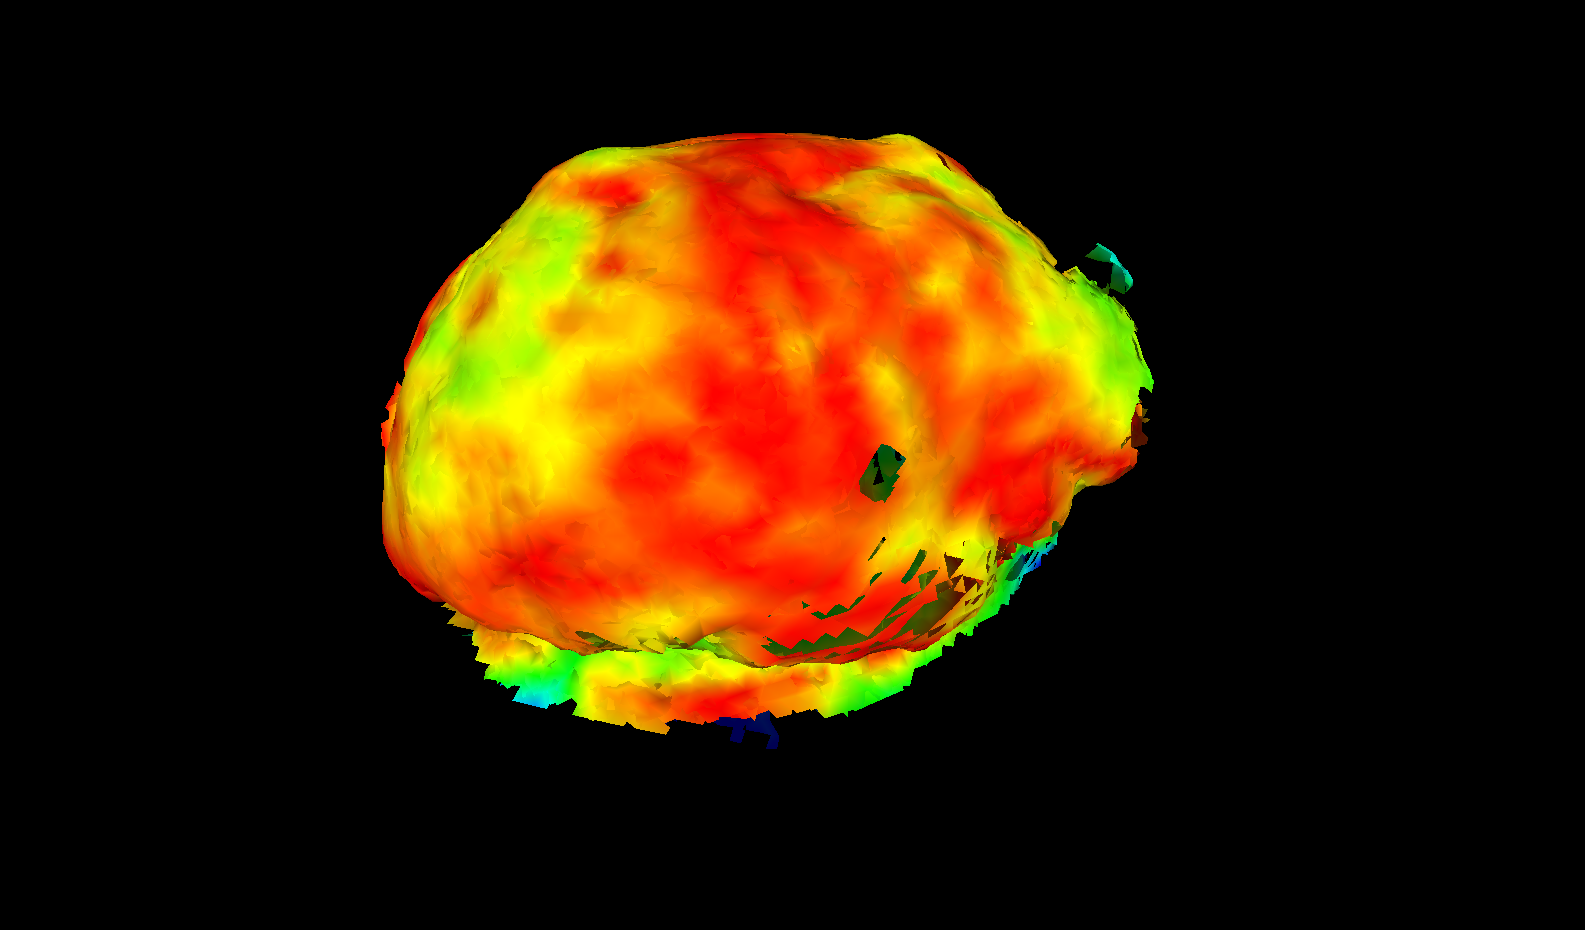
\includegraphics[width=.2\linewidth]{figures/object_recon/hauss/brain.png}&
      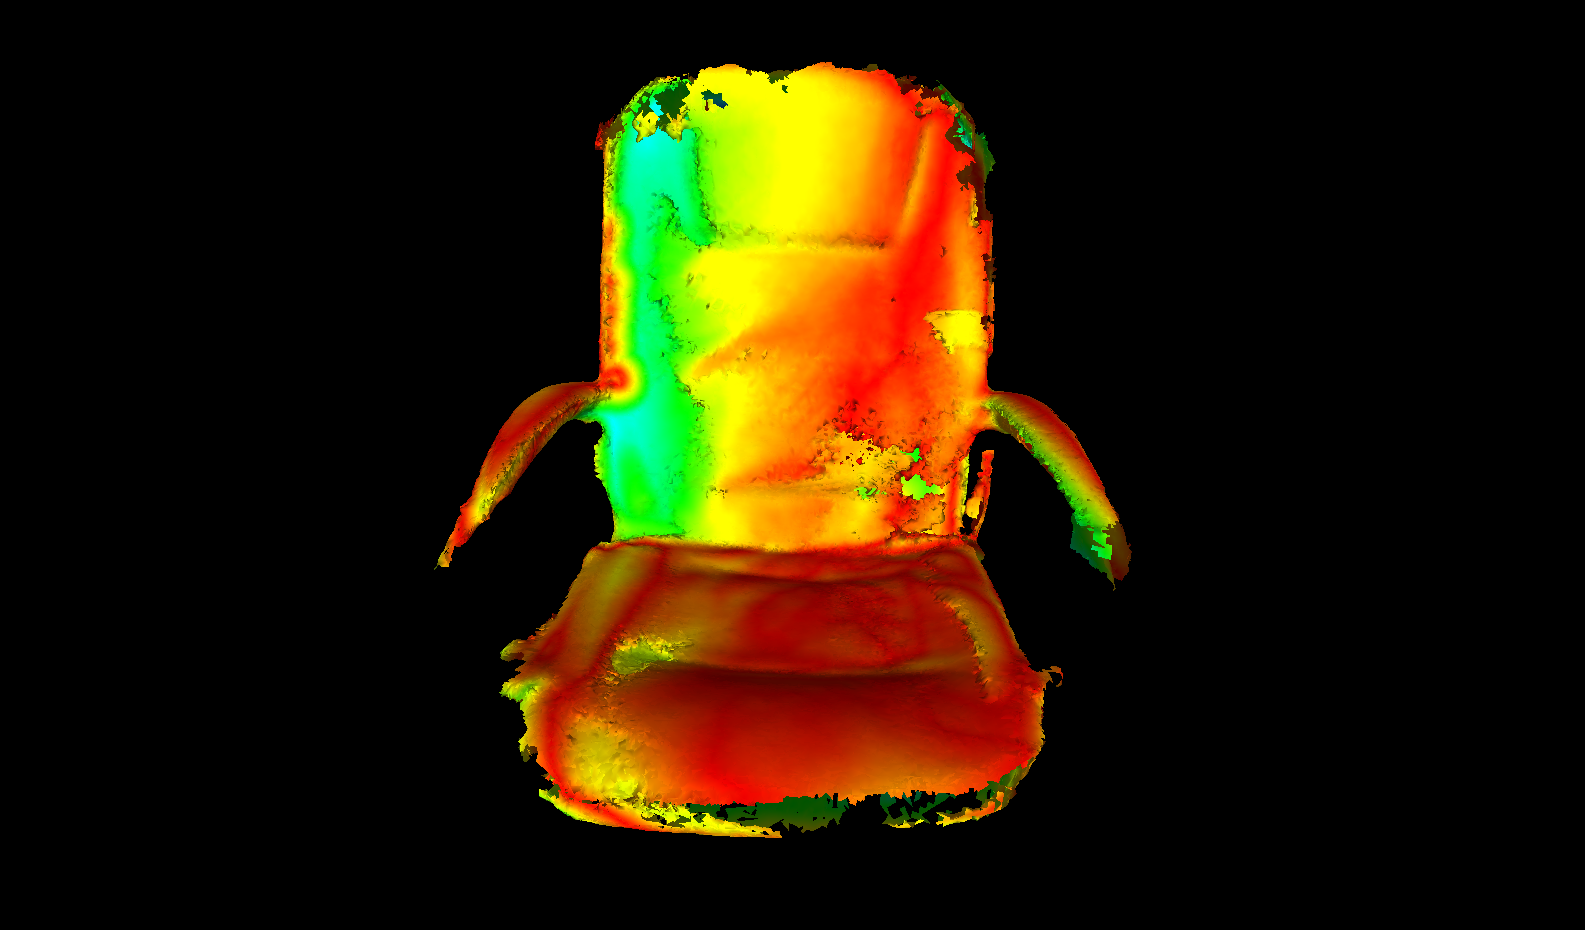
\includegraphics[width=.2\linewidth]{figures/object_recon/hauss/chair.png}&
      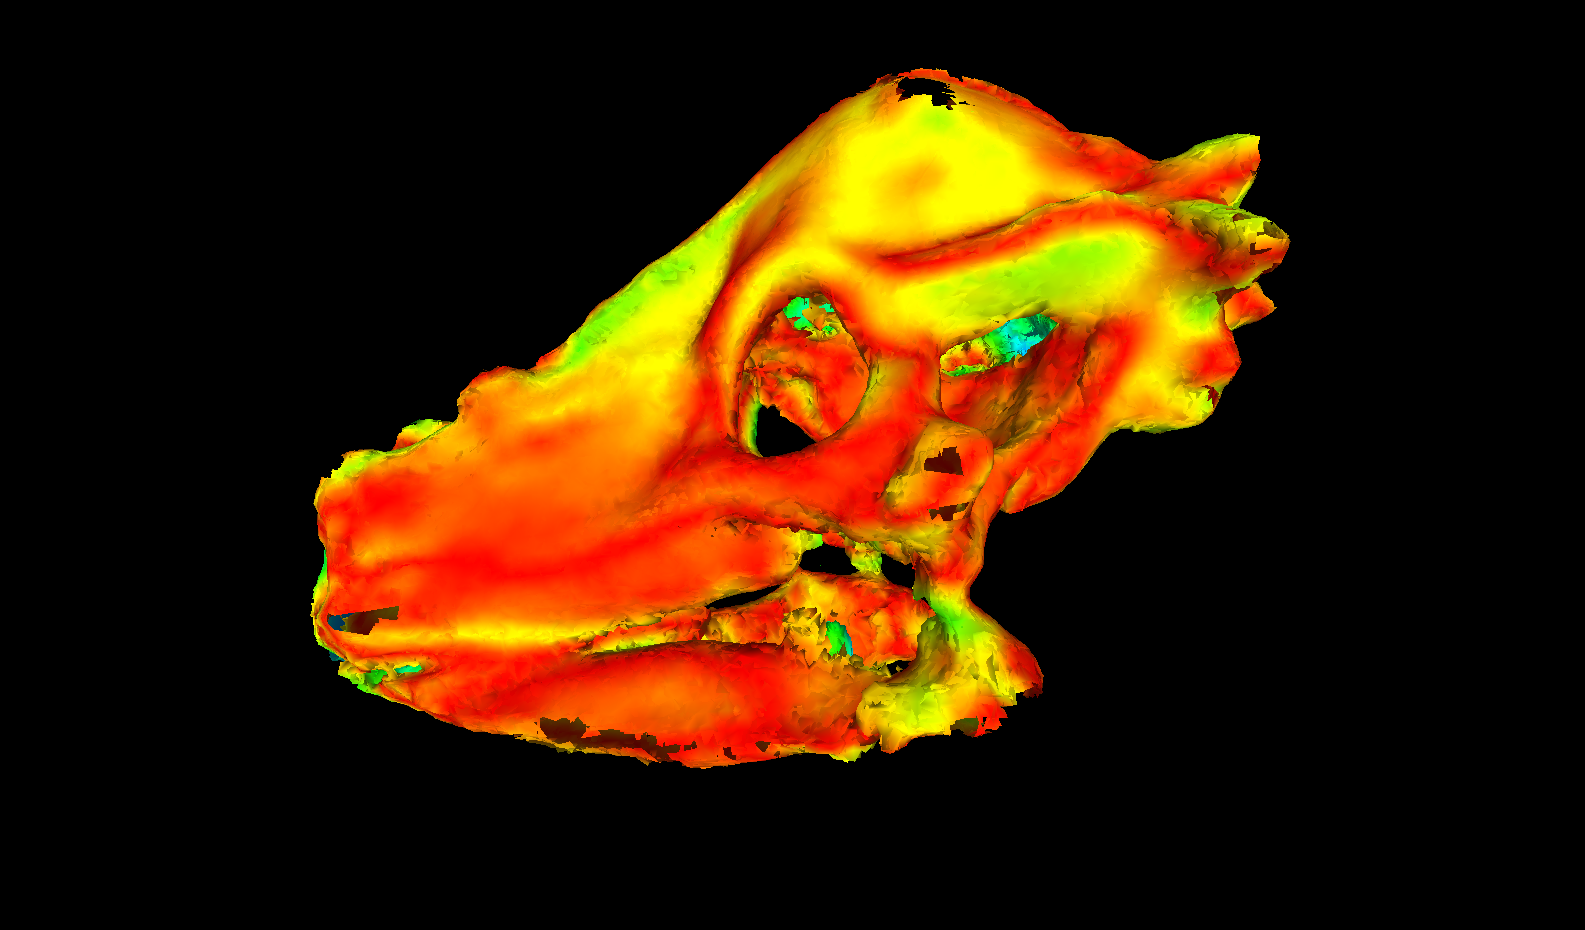
\includegraphics[width=.2\linewidth]{figures/object_recon/hauss/dino.png} \\
      (a) & (b) & (c) & (d) \\
    \end{tabular} \\
    \begin{tabular}{ccc}
      \textit{Max} & 
      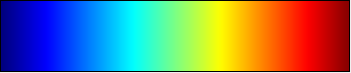
\includegraphics[width=.2\linewidth]{figures/object_recon/hauss/colour_range.png} & 
      \textit{Min} \\
      & (e) & \\
    \end{tabular}
  \end{tabular}
  \caption[Probabilistic Object Reconstruction Hausdorff Distance]
  {Renderings of the sequences evaluated in Table \ref{tbl:probobj_hauss} textured 
  on Hausdorff Distance (a, b, c, d). The minimum and maximum values given in Table 
  \ref{tbl:probobj_hauss} are mapped to the colour range of (e).}
\end{figure}

\section{Discussion}
\label{sec:probobj_discussion}
It is evident from Sections \ref{sec:sec:probobj_qualitative} and \ref{sec:probobj_quantitative} 
that the proposed approach is capable of densely reconstructing a range of rigid objects, providing 
closed and consistent object models, versus the state-of-the-art approach of \textit{Ren et al} 
\cite{Ren2013}, which failed to reconstruct any of the objects with nontrivial geometry that it 
was evaluated on. Additionally, the proposed approach shows an improvement over direct segmentation 
in image space of the object of interest in terms of pose estimation. When evaluating the output 
reconstructions of the proposed system versus those extracted from a standard \textit{KinectFusion} 
like pipeline (post reconstruction), the proposed system is capable of producing reconstructions that 
are geometrically similar.

The probabilistic formulation proposed in this work is intended to be easily generalised, such that 
it may be adapted for a range of use cases. For example, when utilising stereo sensors where a noise 
model may not be known a-priori, the framework allows for a suitable prior to be used. Additionally, 
the proposed approach is intentionally decoupled from the object segmentation model, allowing for 
ease of adaption for multiple object scenarios, or those where a continuous distribution over voxel 
labellings is required.

\chapter{Stereo Shape and Pose Regression}
\section{Introduction}
~\label{sec:spp_introduction}
% Object reconstruction requires full view of object
% Relevant background - pose regression, shape regression
% In the wild, RGBD won't work, hence stereo.
% 

\section{Related Work}
~\label{sec:spp_related}

\section{Algorithmic Overview}
~\label{sec:spp_algorithm}
\subsection{Gaussian Process Marginal Likelihood}
~\label{subsec:spp_gp_marginal_likelihood}
Given a Latent Variable Model of the following form
\begin{equation}
  \label{eqn:spp_gp_lvm}
  P(\bm{Y} \given \bm{X}, \bm{W}, \beta) = P(\bm{Y} \given \bm{WX}^{T}, \beta^{-1}\bm{I})
\end{equation}
Where in Equation~\ref{eqn:spp_gp_lvm} the observed data \(\bm{Y} \in \mathbb{R}^{N \times D}\) 
is mapped to a lower dimensionality manifold \(\bm{X} \in \mathbb{R}^{N \times P}\), by parameters 
\(\bm{W} \in \mathbb{R}^{P \times D}\) and variance \( \beta \).

The marginal likelihood of \(\bm{X}\) is of the form outlined in Equation~\ref{eqn:spp_gp_marginal}.
\begin{equation}
  \label{eqn:spp_gp_marginal}
  P(\bm{Y} \given \bm{X}, \beta) = \int P(\bm{Y} \given \bm{X}, \bm{W}, \beta) P(\bm{W}) \intd{\bm{W}}
\end{equation}
Where in Equation~\ref{eqn:spp_gp_marginal}, \(P(\bm{W})\) is a Gaussian conjugate prior of the 
form \(\mathcal{N}(\bm{W} \given \bm{0}, \bm{I})\).

To find the marginal distribution outlined in Equation~\ref{eqn:spp_gp_marginal}, it's form may 
be simplified as follows in Equation~\ref{}.

\begin{align}
  \label{eqn:spp_gp_marginal_simplify}
  % Line 1.
  P(\bm{Y} \given \bm{X}, \beta) ={}& \int \mathcal{N}(\bm{Y} \given \bm{WX}^{T}, \beta^{-1}\bm{I})
  \mathcal{N}(\bm{W} \given \bm{0}, \bm{I}) \intd{\bm{W}} \\
  % Line 2.
  =& \int \frac{1}{\sqrt{\left|2\pi\beta^{-1}\bm{I}\right|}} \exp{ 
  \Bigg[
    -\frac{\beta}{2} {\big( \bm{Y} - \bm{WX} \big)}^{T} \big( \bm{Y} - \bm{WX} \big) 
  \Bigg]}
  \frac{1}{\sqrt{\left|2\pi\bm{I}\right|}} \exp{ 
  \Bigg[
    -\frac{1}{2} \bm{W}^{T}\bm{W}
  \Bigg]} \intd{\bm{W}} \\
  % Line 3.
  =& \frac{1}{\sqrt{\left|2\pi\beta^{-1}\bm{I}\right|}} \frac{1}{\sqrt{\left|2\pi\bm{I}\right|}} 
  \int \exp{
  \Bigg[
    -\frac{\beta}{2} {\big( \bm{Y} - \bm{WX} \big)}^{T} \big( \bm{Y} - \bm{WX} \big) 
    -\frac{1}{2} \bm{W}^{T}\bm{W}
  \Bigg]} \intd{\bm{W}} \\
  % Line 4.
  \propto& \int \exp{
  \Bigg[
    -\frac{\beta}{2} {\big( \bm{Y} - \bm{WX} \big)}^{T} \big( \bm{Y} - \bm{WX} \big) 
    -\frac{1}{2} \bm{W}^{T}\bm{W}
  \Bigg]} \intd{\bm{W}} \\
  % Line 5.
  \propto& \int \exp{ 
  \Bigg[ -\frac{1}{2} \Big[
    \beta {\big( \bm{Y} - \bm{X}^{T}\bm{W} \big)}^{T} \big( \bm{Y} - \bm{X}^{T}\bm{W} \big) 
    + \bm{W}^{T}\bm{W}
  \Big] \Bigg]} \intd{\bm{W}} \\
  % Line 6.
  \propto& \exp{\Bigg[ -\frac{\beta}{2} \bm{Y}^{T}\bm{Y} \Bigg]} 
  \int \exp{
  \Bigg[ -\frac{1}{2} \Big[
    -\beta \big( \bm{Y}^{T}\bm{X}^{T}\bm{W} \big) 
    -\beta {\big( \bm{W}^{T}\bm{XY} \big)}^{T}
    +\beta \bm{W}^{T}\bm{XX}^{T}\bm{W}
    + \bm{W}^{T}\bm{W}\Big] \Bigg]} \intd{\bm{W}} \\
  % Line 7.
  \propto& \exp{\Bigg[ -\frac{\beta}{2} \bm{Y}^{T}\bm{Y} \Bigg]} 
  \int \exp{
  \Bigg[ -\frac{1}{2} \Big[
    -2\beta \bm{Y}^{T}\bm{X}^{T}\bm{W}
    +\beta \bm{W}^{T}\bm{XX}^{T}\bm{W}
    + \bm{W}^{T}\bm{W}
  \Big] \Bigg]} \intd{\bm{W}} \\
  % Line 7.
  \propto& \exp{\Bigg[ -\frac{\beta}{2} \bm{Y}^{T}\bm{Y} \Bigg]} 
  \int \exp{
  \Bigg[ -\frac{1}{2} \Big[
    \bm{W}^{T} \big( \beta \bm{XX}^{T} + \bm{I} \big) \bm{W}
    -2\beta \bm{Y}^{T}\bm{X}^{T}\bm{W}
  \Big] \Bigg]} \intd{\bm{W}}
\end{align}

To make the integral over \(\bm{W}\) tractable in Equation~\ref{eqn:spp_gp_marginal_simplify}, 
the distribution \(P(\bm{Y} \given \bm{X}, \beta)\) must be of a Gaussian form; an exponential 
of a quadratic form. Completing the square in \(\bm{W}\) allows the marginal to be expressed 
in such a form. First, making the change of variables as in Equation 
~\ref{eqn:spp_gp_marginal_change}, the procedure is as follows in Equation~\ref{eqn:spp_gp_complete}.

\begin{align}
  \label{eqn:spp_gp_marginal_change}
  \bm{A} ={}& \beta \bm{XX}^{T} + \bm{I}\\
  \bm{b} =& \beta \bm{Y}^{T} \bm{X}^{T}
\end{align}
a
\begin{align}
  \label{eqn:spp_gp_complete}
  % Line 1.
  P(\bm{Y} \given \bm{X}, \beta) \propto{}& \exp{\Big[ -\frac{\beta}{2}\bm{Y}^{T}\bm{Y} \Big]}
  \int \exp{\Big[ -\frac{1}{2} 
  \big[
    \bm{W}^{T}\bm{AW} - 2\bm{bW}  
  \big]
  \Big]} \intd{\bm{W}}\\
  % Line 2.
  \propto& \exp{\Big[ -\frac{\beta}{2}\bm{Y}^{T}\bm{Y} \Big]}
  \int \exp{\Big[ 
    -\frac{1}{2} \bm{W}^{T}\bm{AW} 
    - 2\bm{bW} 
    - \bm{b}^{T}\bm{A}^{-1}\bm{b}  
  \Big]} \intd{\bm{W}}\\
  % Line 3.
  \propto& \exp{\Big[ -\frac{\beta}{2}\bm{Y}^{T}\bm{Y} \Big]}
  \int \exp{\Big[ 
    -\frac{1}{2} \bm{W}^{T}\bm{AW} 
    - 2\bm{bA}\bm{A}^{-1}\bm{W}
    + \bm{b}^{T}\bm{A}^{-1}\bm{AA}^{-1}\bm{b}  
  \Big]} \intd{\bm{W}}\\
  % Line 4.
  \propto& \exp{\Big[ -\frac{\beta}{2}\bm{Y}^{T}\bm{Y} \Big]}
  \int \exp{\Big[ -\frac{1}{2} \big[ 
      {\big( \bm{W} - \bm{A}^{-1}\bm{b} \big)}^{T}
      \bm{A}
      \big( \bm{W} - \bm{A}^{-1}\bm{b} \big)
      - \bm{b}^{T}\bm{A}^{-1}\bm{b}
    \big]
  \Big]} \intd{\bm{W}}\\
  % Line 5.
  \propto& \exp{\Big[ -\frac{\beta}{2}\bm{Y}^{T}\bm{Y} \Big]}
  \exp{\Big[ -\frac{1}{2} \big[
      \sqrt{\left| 2 \pi \bm{A} \right|}
      - \bm{b}^{T}\bm{A}^{-1}\bm{b}
    \big]
  \Big]}\\
  % Line 6.
  \propto& \exp{\Big[ \frac{1}{2} \big[
    \beta \bm{Y}^{T} \beta \bm{Y}
    - \bm{b}^{T}\bm{A}^{-1}\bm{b}
    \big]
  \Big]}\\
  % Line 7.
  \propto& \exp{\Big[ -\frac{1}{2}
  \bm{Y}^{T} \big(
    \beta \bm{I} - \beta^{2}\bm{X}^{T}\bm{A}^{-1}\bm{X}
    \big)\bm{Y}
  \Big]}
\end{align}

With the distribution \(P(\bm{Y} \given \bm{X}, \beta)\) derived as being proportional to  
an exponentiated quadratic form as in Equation~\ref{eqn:spp_gp_complete}, it is 
clear that the inverse covariance matrix \(\bm{\Sigma}^{-1}\) of the Gaussian distribution 
corresponding to \(P(\bm{Y} \given \bm{X}, \beta)\) is as follows in Equation 
~\ref{eqn:spp_sig_inv}.

\begin{align}
  \label{eqn:spp_sig_inv}
  \bm{\Sigma}^{-1} ={}& \beta \bm{I} - \beta^{2} \bm{X}^{T} \bm{A}^{-1} \bm{X}\\
  =& \beta \bm{I} - \beta^{2} \bm{X}^{T} {\big(\beta \bm{XX}^{T} + \bm{I} \big)}^{-1}
\end{align}

\section{Qualitative Results}
~\label{sec:spp_qualitative}

\section{Quantitative Results}
~\label{sec:spp_quantitative}

\begin{appendices}
  \section{Mathematical Appendices}
  \begin{landscape}
\subsection{Rodriguez Paramaterisation Partial Derivatives}
In this section the full Partial Derivatives of a Rotation Matrix \(\bm{R}\)
generated by the Formulation of Equation~\ref{eqn:rodriguez_matrix_eq} in
Section~\ref{subsec:moseg_static_camera_tracking} are given as follows.
\begin{equation}
  \label{eqn:rodrigues_full_alpha_deriv}
  \frac{\partial \bm{R}}{\partial \alpha} =
  % BEGIN SYMPY LATEX OUTPUT.
    \begin{bmatrix}
      - \frac{2 \alpha \left(\alpha^{2} - \beta^{2} - \gamma^{2} +
          1\right)}{{\left(\alpha^{2} + \beta^{2} + \gamma^{2} + 1\right)}^{2}} +
      \frac{2 \alpha}{\alpha^{2} + \beta^{2} + \gamma^{2} + 1} &
      - \frac{2 \alpha \left(2 \alpha \beta + \gamma\right)}{{\left(\alpha^{2} +
          \beta^{2} + \gamma^{2} + 1\right)}^{2}} + \frac{2 \beta}{\alpha^{2} +
        \beta^{2} + \gamma^{2} + 1} &
      - \frac{2 \alpha \left(2 \alpha \gamma - \beta\right)}{{{\left(\alpha^{2} +
          \beta^{2} + \gamma^{2} + 1\right)}}^{2}}
      + \frac{2 \gamma}{\alpha^{2} + \beta^{2} + \gamma^{2} + 1}\\
      -\frac{2 \alpha \left(2 \alpha \beta - \gamma\right)}{{\left(\alpha^{2} +
          \beta^{2} + \gamma^{2} + 1\right)}^{2}} + \frac{2 \beta}{\alpha^{2} +
        \beta^{2} + \gamma^{2} + 1} &
      \frac{2 \alpha \left(\alpha^{2} - \beta^{2} + \gamma^{2} - 1\right)}
      {{\left(\alpha^{2} + \beta^{2} + \gamma^{2} + 1\right)}^{2}} - \frac{2 \alpha}
      {\alpha^{2} + \beta^{2} + \gamma^{2} + 1} &
      - \frac{2 \alpha \left(\alpha + 2 \beta \gamma\right)}
      {{\left(\alpha^{2} + \beta^{2} + \gamma^{2} + 1\right)}^{2}} +
      \frac{1}{\alpha^{2} + \beta^{2} + \gamma^{2} + 1}\\
      - \frac{2 \alpha \left(2 \alpha \gamma + \beta\right)}{{\left(\alpha^{2} +
          \beta^{2} + \gamma^{2} + 1\right)}^{2}} + \frac{2 \gamma}{\alpha^{2} +
        \beta^{2} + \gamma^{2} + 1} &
      \frac{2 \alpha \left(\alpha - 2 \beta \gamma\right)}
      {{\left(\alpha^{2} + \beta^{2} + \gamma^{2} + 1\right)}^{2}} -
      \frac{1}{\alpha^{2} + \beta^{2} + \gamma^{2} + 1} &
      \frac{2 \alpha \left(\alpha^{2} + \beta^{2} - \gamma^{2} - 1\right)}
      {{\left(\alpha^{2} + \beta^{2} + \gamma^{2} + 1\right)}^{2}} - \frac{2 \alpha}
      {\alpha^{2} + \beta^{2} + \gamma^{2} + 1}
    \end{bmatrix}
    % END SYMPY LATEX OUTPUT.
\end{equation}

\begin{equation}
  \label{eqn:rodrigues_full_beta_deriv}
  \frac{\partial \bm{R}}{\partial \beta} =
  % BEGIN SYMPY LATEX OUTPUT.
  \begin{bmatrix}
    - \frac{2 \beta \left(\alpha^{2} - \beta^{2} - \gamma^{2} + 1\right)}
    {{\left(\alpha^{2} + \beta^{2} + \gamma^{2} + 1\right)}^{2}} - \frac{2 \beta}
    {\alpha^{2} + \beta^{2} + \gamma^{2} + 1} &
    \frac{2 \alpha}{\alpha^{2} + \beta^{2} + \gamma^{2} + 1} - \frac{2 \beta
      \left(2 \alpha \beta + \gamma\right)}{{\left(\alpha^{2} + \beta^{2} +
        \gamma^{2} + 1\right)}^{2}} &
    - \frac{2 \beta \left(2 \alpha \gamma - \beta\right)}{{\left(\alpha^{2} +
        \beta^{2} + \gamma^{2} + 1\right)}^{2}} - \frac{1}{\alpha^{2} + \beta^{2} +
      \gamma^{2} + 1}\\
    \frac{2 \alpha}{\alpha^{2} + \beta^{2} + \gamma^{2} + 1} - \frac{2 \beta
      \left(2 \alpha \beta - \gamma\right)}{{\left(\alpha^{2} + \beta^{2} +
        \gamma^{2} + 1\right)}^{2}} &
    \frac{2 \beta \left(\alpha^{2} - \beta^{2} + \gamma^{2} - 1\right)}
    {{\left(\alpha^{2} + \beta^{2} + \gamma^{2} + 1\right)}^{2}} + \frac{2 \beta}
    {\alpha^{2} + \beta^{2} + \gamma^{2} + 1} &
    - \frac{2 \beta \left(\alpha + 2 \beta \gamma\right)}{{\left(\alpha^{2} +
        \beta^{2} + \gamma^{2} + 1\right)}^{2}} + \frac{2 \gamma}{\alpha^{2} +
      \beta^{2} + \gamma^{2} + 1}\\
    - \frac{2 \beta \left(2 \alpha \gamma + \beta\right)}{{\left(\alpha^{2} +
        \beta^{2} + \gamma^{2} + 1\right)}^{2}} + \frac{1}{\alpha^{2} + \beta^{2} +
      \gamma^{2} + 1} &
    \frac{2 \beta \left(\alpha - 2 \beta \gamma\right)}{{\left(\alpha^{2} +
        \beta^{2} + \gamma^{2} + 1\right)}^{2}} + \frac{2 \gamma}{\alpha^{2} +
      \beta^{2} + \gamma^{2} + 1} &
    \frac{2 \beta \left(\alpha^{2} + \beta^{2} - \gamma^{2} - 1\right)}
    {{\left(\alpha^{2} + \beta^{2} + \gamma^{2} + 1\right)}^{2}} - \frac{2 \beta}
    {\alpha^{2} + \beta^{2} + \gamma^{2} + 1}
  \end{bmatrix}
  % END SYMPY LATEX OUTPUT.
\end{equation}

\begin{equation}
  \label{eqn:rodrigues_full_gamma_deriv}
  \frac{\partial \bm{R}}{\partial \gamma} =
  % BEGIN SYMPY LATEX OUTPUT.
  \begin{bmatrix}
    - \frac{2 \gamma \left(\alpha^{2} - \beta^{2} - \gamma^{2} + 1\right)}
    {{\left(\alpha^{2} + \beta^{2} + \gamma^{2} + 1\right)}^{2}} - \frac{2 \gamma}
    {\alpha^{2} + \beta^{2} + \gamma^{2} + 1} &
    - \frac{2 \gamma \left(2 \alpha \beta + \gamma\right)}{{\left(\alpha^{2} +
        \beta^{2} + \gamma^{2} + 1\right)}^{2}} + \frac{1}{\alpha^{2} + \beta^{2} +
      \gamma^{2} + 1} &
    \frac{2 \alpha}{\alpha^{2} + \beta^{2} + \gamma^{2} + 1} - \frac{2 \gamma
      \left(2 \alpha \gamma - \beta\right)}{{\left(\alpha^{2} + \beta^{2} +
        \gamma^{2} + 1\right)}^{2}}\\
    - \frac{2 \gamma \left(2 \alpha \beta - \gamma\right)}{{\left(\alpha^{2} +
        \beta^{2} + \gamma^{2} + 1\right)}^{2}} - \frac{1}{\alpha^{2} + \beta^{2} +
      \gamma^{2} + 1} &
    \frac{2 \gamma \left(\alpha^{2} - \beta^{2} + \gamma^{2} - 1\right)}
    {{\left(\alpha^{2} + \beta^{2} + \gamma^{2} + 1\right)}^{2}} - \frac{2 \gamma}
    {\alpha^{2} + \beta^{2} + \gamma^{2} + 1} &
    \frac{2 \beta}{\alpha^{2} + \beta^{2} + \gamma^{2} + 1} - \frac{2 \gamma
      \left(\alpha + 2 \beta \gamma\right)}{{\left(\alpha^{2} + \beta^{2} +
        \gamma^{2} + 1\right)}^{2}}\\
    \frac{2 \alpha}{\alpha^{2} + \beta^{2} + \gamma^{2} + 1} - \frac{2 \gamma
      \left(2 \alpha \gamma + \beta\right)}{{\left(\alpha^{2} + \beta^{2} +
        \gamma^{2} + 1\right)}^{2}} &
    \frac{2 \beta}{\alpha^{2} + \beta^{2} + \gamma^{2} + 1} + \frac{2 \gamma
      \left(\alpha - 2 \beta \gamma\right)}{{\left(\alpha^{2} + \beta^{2} +
        \gamma^{2} + 1\right)}^{2}} &
    \frac{2 \gamma \left(\alpha^{2} + \beta^{2} - \gamma^{2} - 1\right)}
    {{\left(\alpha^{2} + \beta^{2} + \gamma^{2} + 1\right)}^{2}} + \frac{2 \gamma}
    {\alpha^{2} + \beta^{2} + \gamma^{2} + 1}
  \end{bmatrix}
  % END SYMPY LATEX OUTPUT.
\end{equation}
\end{landscape}

  \section{Motion Segmentation Results Appendices}
  \subsection{Motion Segmentation additional ATE results}
In this section, additional results for the Motion Segmentation system
to complement those outlined in Section~\ref{sec:moseg_quantitative} are given.
The results in this section assess Absolute Trajectory Error on the TUM Dynamic
Objects \textit{Validation} set. Quantitative results are given in Table
~\ref{tbl:moseg_ate_validation} and visualised in Figure
~\ref{fig:moseg_ate_validation}.

\begin{table}[!htbp]
~\label{tbl:moseg_ate_validation}
\begin{center}
  \begin{tabular}{l@{\hskip 1cm} c c}
    \emph{TUM Standard Sequence Name} & \emph{MoSeg} ATE & \emph{Baseline} ATE \\
    \midrule
    \textsf{fr3-sitting-static} & 0.046 \std{0.021} & \textbf{0.030 \std{0.014}}\\
    \textsf{fr3-sitting-xyz} & 0.048 \std{0.027} & 0.048 \std{0.027}\\
    \textsf{fr3-sitting-halfsphere} & 0.029 \std{0.013} & \textbf{0.028 \std{0.012}}\\
    \textsf{fr3-sitting-rpy} & 0.047 \std{0.022} & \textbf{0.044 \std{0.020}}\\
    \textsf{fr3-walking-static} & \textbf{0.163 \std{0.191}} & 0.466 \std{0.252}\\
    \textsf{fr3-walking-xyz} & \textbf{0.092 \std{0.075}} & 0.633 \std{0.429}\\
    \textsf{fr3-walking-halfsphere} & \textbf{0.412 \std{0.271}} & 0.525 \std{0.325}\\
    \textsf{fr3-walking-rpy} & \textbf{0.082 \std{0.042}} & 0.561 \std{0.182}\\
  \end{tabular}
\end{center}
\caption[Motion Segmentation ATE Validation Set]
{The Absolute Trajectory Error (ATE) results (in metres, lower is better) 
achieved by the proposed approach in comparison to the baseline InfiniTAM
~\cite{Prisacariu2014} framework on a variety of the standard sequences from
  the TUM RGBD \textit{Validation} dataset~\cite{Sturm2012}. Results are in the
  format mean \( \pm \) standard deviation. The better result (by mean) on each
  sequence is highlighted in bold.}
\end{table}

\begin{figure}[!htbp]
~\label{fig:moseg_ate_validation}
  \centering
  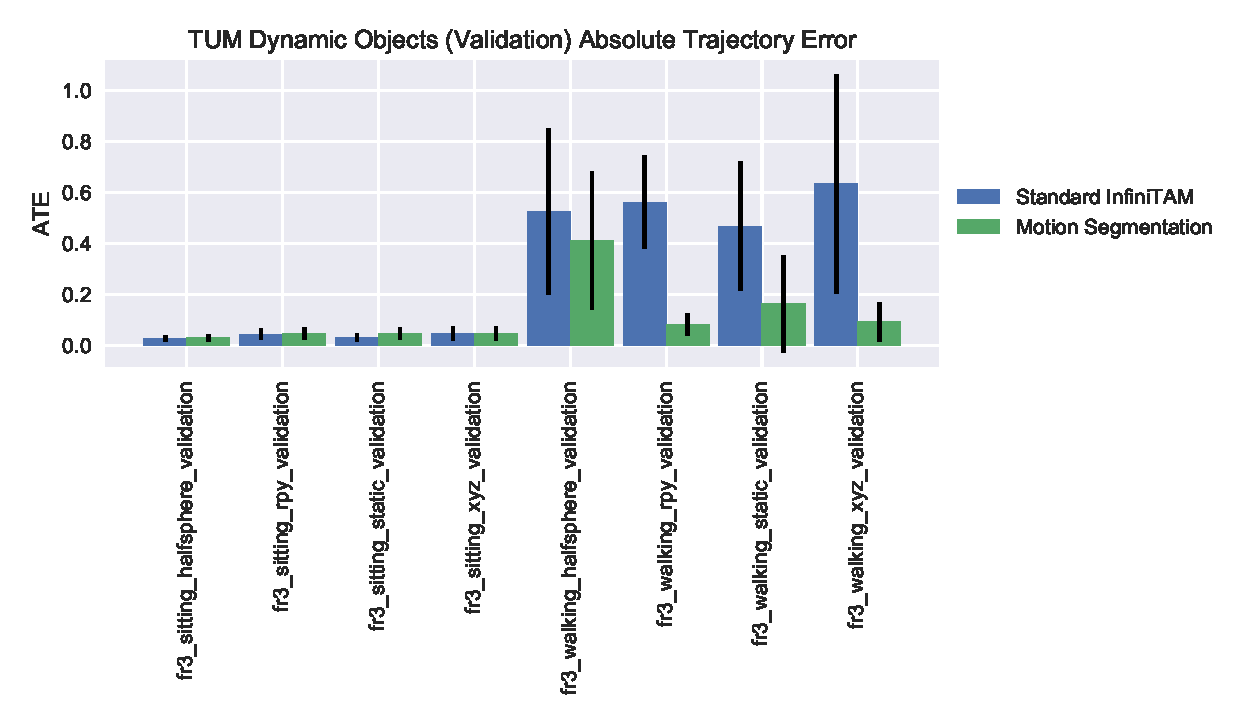
\includegraphics[width=\linewidth]{figures/moseg/ate_validation.eps}
  \caption[Motion Segmentation ATE Validation Set]
  {Absolute Trajectory Error for the TUM Dynamic Scenes
    \textit{Validation} dataset.}
\end{figure}

\subsection{Motion Segmentation additional RTE results}
In this section, additional results for the Motion Segmentation system
to complement those outlined in Section~\ref{sec:moseg_quantitative} are given.
The results in this section assess Relative Trajectory Error on the TUM Dynamic
Objects \textit{Validation} set. Quantitative results are given in Table
~\ref{tbl:moseg_rte_validation} and visualised in Figure
~\ref{fig:moseg_rte_validation}.

\begin{table}[!htbp]
~\label{tbl:moseg_rte_validation}
\begin{center}
  \begin{tabular}{l@{\hskip 1cm} c c}
    \emph{TUM Standard Sequence Name} & \emph{MoSeg} RTE & \emph{Baseline} RTE \\
    \midrule
    \textsf{fr3-sitting-static} & 0.013 \std{0.007} & \textbf{0.011 \std{0.007}}\\
    \textsf{fr3-sitting-xyz} & \textbf{0.033 \std{0.021}} & 0.034 \std{0.021}\\
    \textsf{fr3-sitting-halfsphere} & 0.022 \std{0.013} & 0.022 \std{0.012}\\
    \textsf{fr3-sitting-rpy} & 0.05 \std{0.048} & \textbf{0.048 \std{0.043}}\\
    \textsf{fr3-walking-static} & \textbf{0.099 \std{0.240}} & 0.163 \std{0.308}\\
    \textsf{fr3-walking-xyz} & \textbf{0.055 \std{0.039}} & 0.285 \std{0.337}\\
    \textsf{fr3-walking-halfsphere} & \textbf{0.171 \std{0.324}} & 0.211 \std{0.233}\\
    \textsf{fr3-walking-rpy} & \textbf{0.139 \std{0.067}} & 0.194 \std{0.182}\\
  \end{tabular}
\end{center}
\caption[Motion Segmentation RTE Validation Set]
{The Relative Trajectory Error (RTE) results (in metres, lower is better) 
achieved by the proposed approach in comparison to the baseline InfiniTAM
~\cite{Prisacariu2014} framework on a variety of the standard sequences from
the TUM RGBD \textit{Validation} dataset~\cite{Sturm2012}. Results are in the
format mean \( \pm \) standard deviation. The better result (by mean) on each
sequence is highlighted in bold.}
\end{table}

\begin{figure}[!htbp]
~\label{fig:moseg_rte_validation}
  \centering
  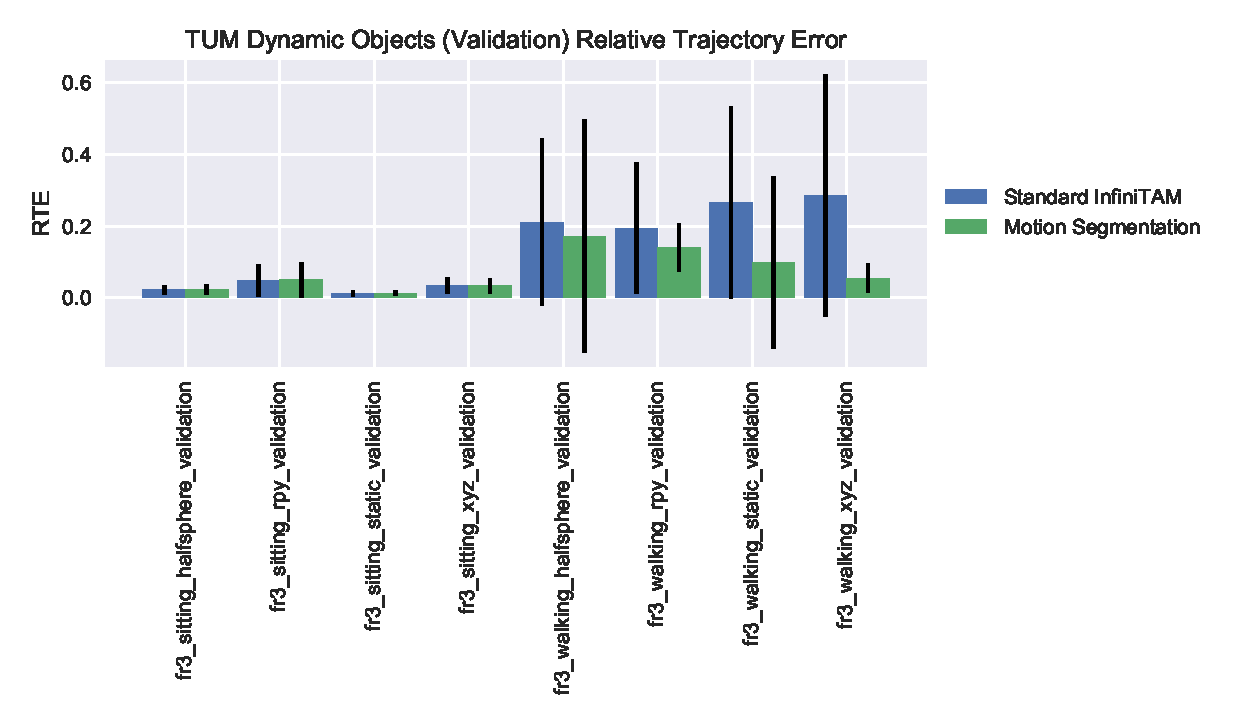
\includegraphics[width=\linewidth]{figures/moseg/rte_validation.eps}
  \caption[Motion Segmentation RTE Validation Set]
  {Relative Trajectory Error for the TUM Dynamic Scenes
    \textit{Validation} dataset.}
\end{figure}
\end{appendices}

\bibliography{bib/definitions,bib/books,bib/slam_moseg,bib/segmentation,bib/objects,bib/ml}
\end{document}